\chapter{Marco  Teórico}\label{chapter:theory}

%En el presente capítulo se introducen los conceptos necesarios para entender la propuesta de esta tesis.

En el presente capítulo se introducen los conceptos fundamentales sobre dispositivos fotónicos y optimización. Primero, se describen los dos dispositivos a optimizar: (i) \emph{bend} y (ii) WDM.
Segundo, se explica la parametrización de estos dispositivos mediante un enfoque basado en píxeles.
Tercero, se brindan detalles necesarios para simular nuestros diseños utilizando el software de modelamiento SPINS-B \citep{Su2020}.
Cuarto, se detallan dos transformaciones comúnmente utilizadas en la optimización topológica robusta: 
(i) filtro por densidad y (ii) proyección.
Finalmente, se describen ocho algoritmos de optimización utilizados en este trabajo.

\section{Dispositivos Fotónicos}

Al estudiar dispositivos fotónicos es de especial interés: i) la
distribución del campo eléctrico, y ii) la transmitancia.

\noindent\textbf{Distribución del campo eléctrico ($\boldsymbol{E}$).} Este nos permite visualizar la distribución de la energía en un dispositivo calculando lo siguiente:

\begin{equation}
  |\boldsymbol{E}|^2 = |\boldsymbol{E_x}|^2+|\boldsymbol{E_y}|^2+|\boldsymbol{E_z}|^2,
\label{eq:field}
\end{equation}

\noindent donde $\boldsymbol{E_x}, \boldsymbol{E_y}, \boldsymbol{E_z}$ representan las componentes del campo eléctrico
en los ejes $x, y, z$, respectivamente
\citep{LukasChrostowski2010}. Observar en una gráfica el valor de $|\boldsymbol{E}|^2$ nos ayuda a entender el funcionamiento de un dispositivo.

\noindent \textbf{Transmitancia $(T)$.} Una manera de cuantificar el correcto funcionamiento de un diseño es mediante el cálculo de $(T)$.
Este valor se define como la relación entre la potencia del flujo que sale del dispositivo con la 
potencia del flujo que ingresa \citep{Christiansen2021}.

En este trabajo estudiamos dos dispositivos fotónicos fundamentales:
(i) \emph{bend} y (ii) \emph{wavelength demultiplexer}.

\subsection{\emph{Bend}}

Un \emph{bend} es un dispositivo fotónico que busca cambiar la dirección de propagación de un haz de ondas.
Un \emph{bend} convencional consiste en una una guía de onda horizontal usada como entrada y
una guía de onda vertical usada como salida, estas son conectadas por una guía de onda con la forma de un
cuarto de circunferencia de radio $r$ y con el mismo grosor de las guías de onda de entrada y salida. La \autoref{fig:efield} presenta un \emph{bend} convencional de radio $r = 1 \mu m$. Se observa que la parte significativa de la energía se pierde en la región curva.
Esto se debe a que el radio de curvatura es muy pequeño, con un valor más grande (e.g., $r = 10 \mu m$) 
las pérdidas se vuelven casi nulas \citep{LukasChrostowski2010}.

\begin{figure}[ht]
  \centering
  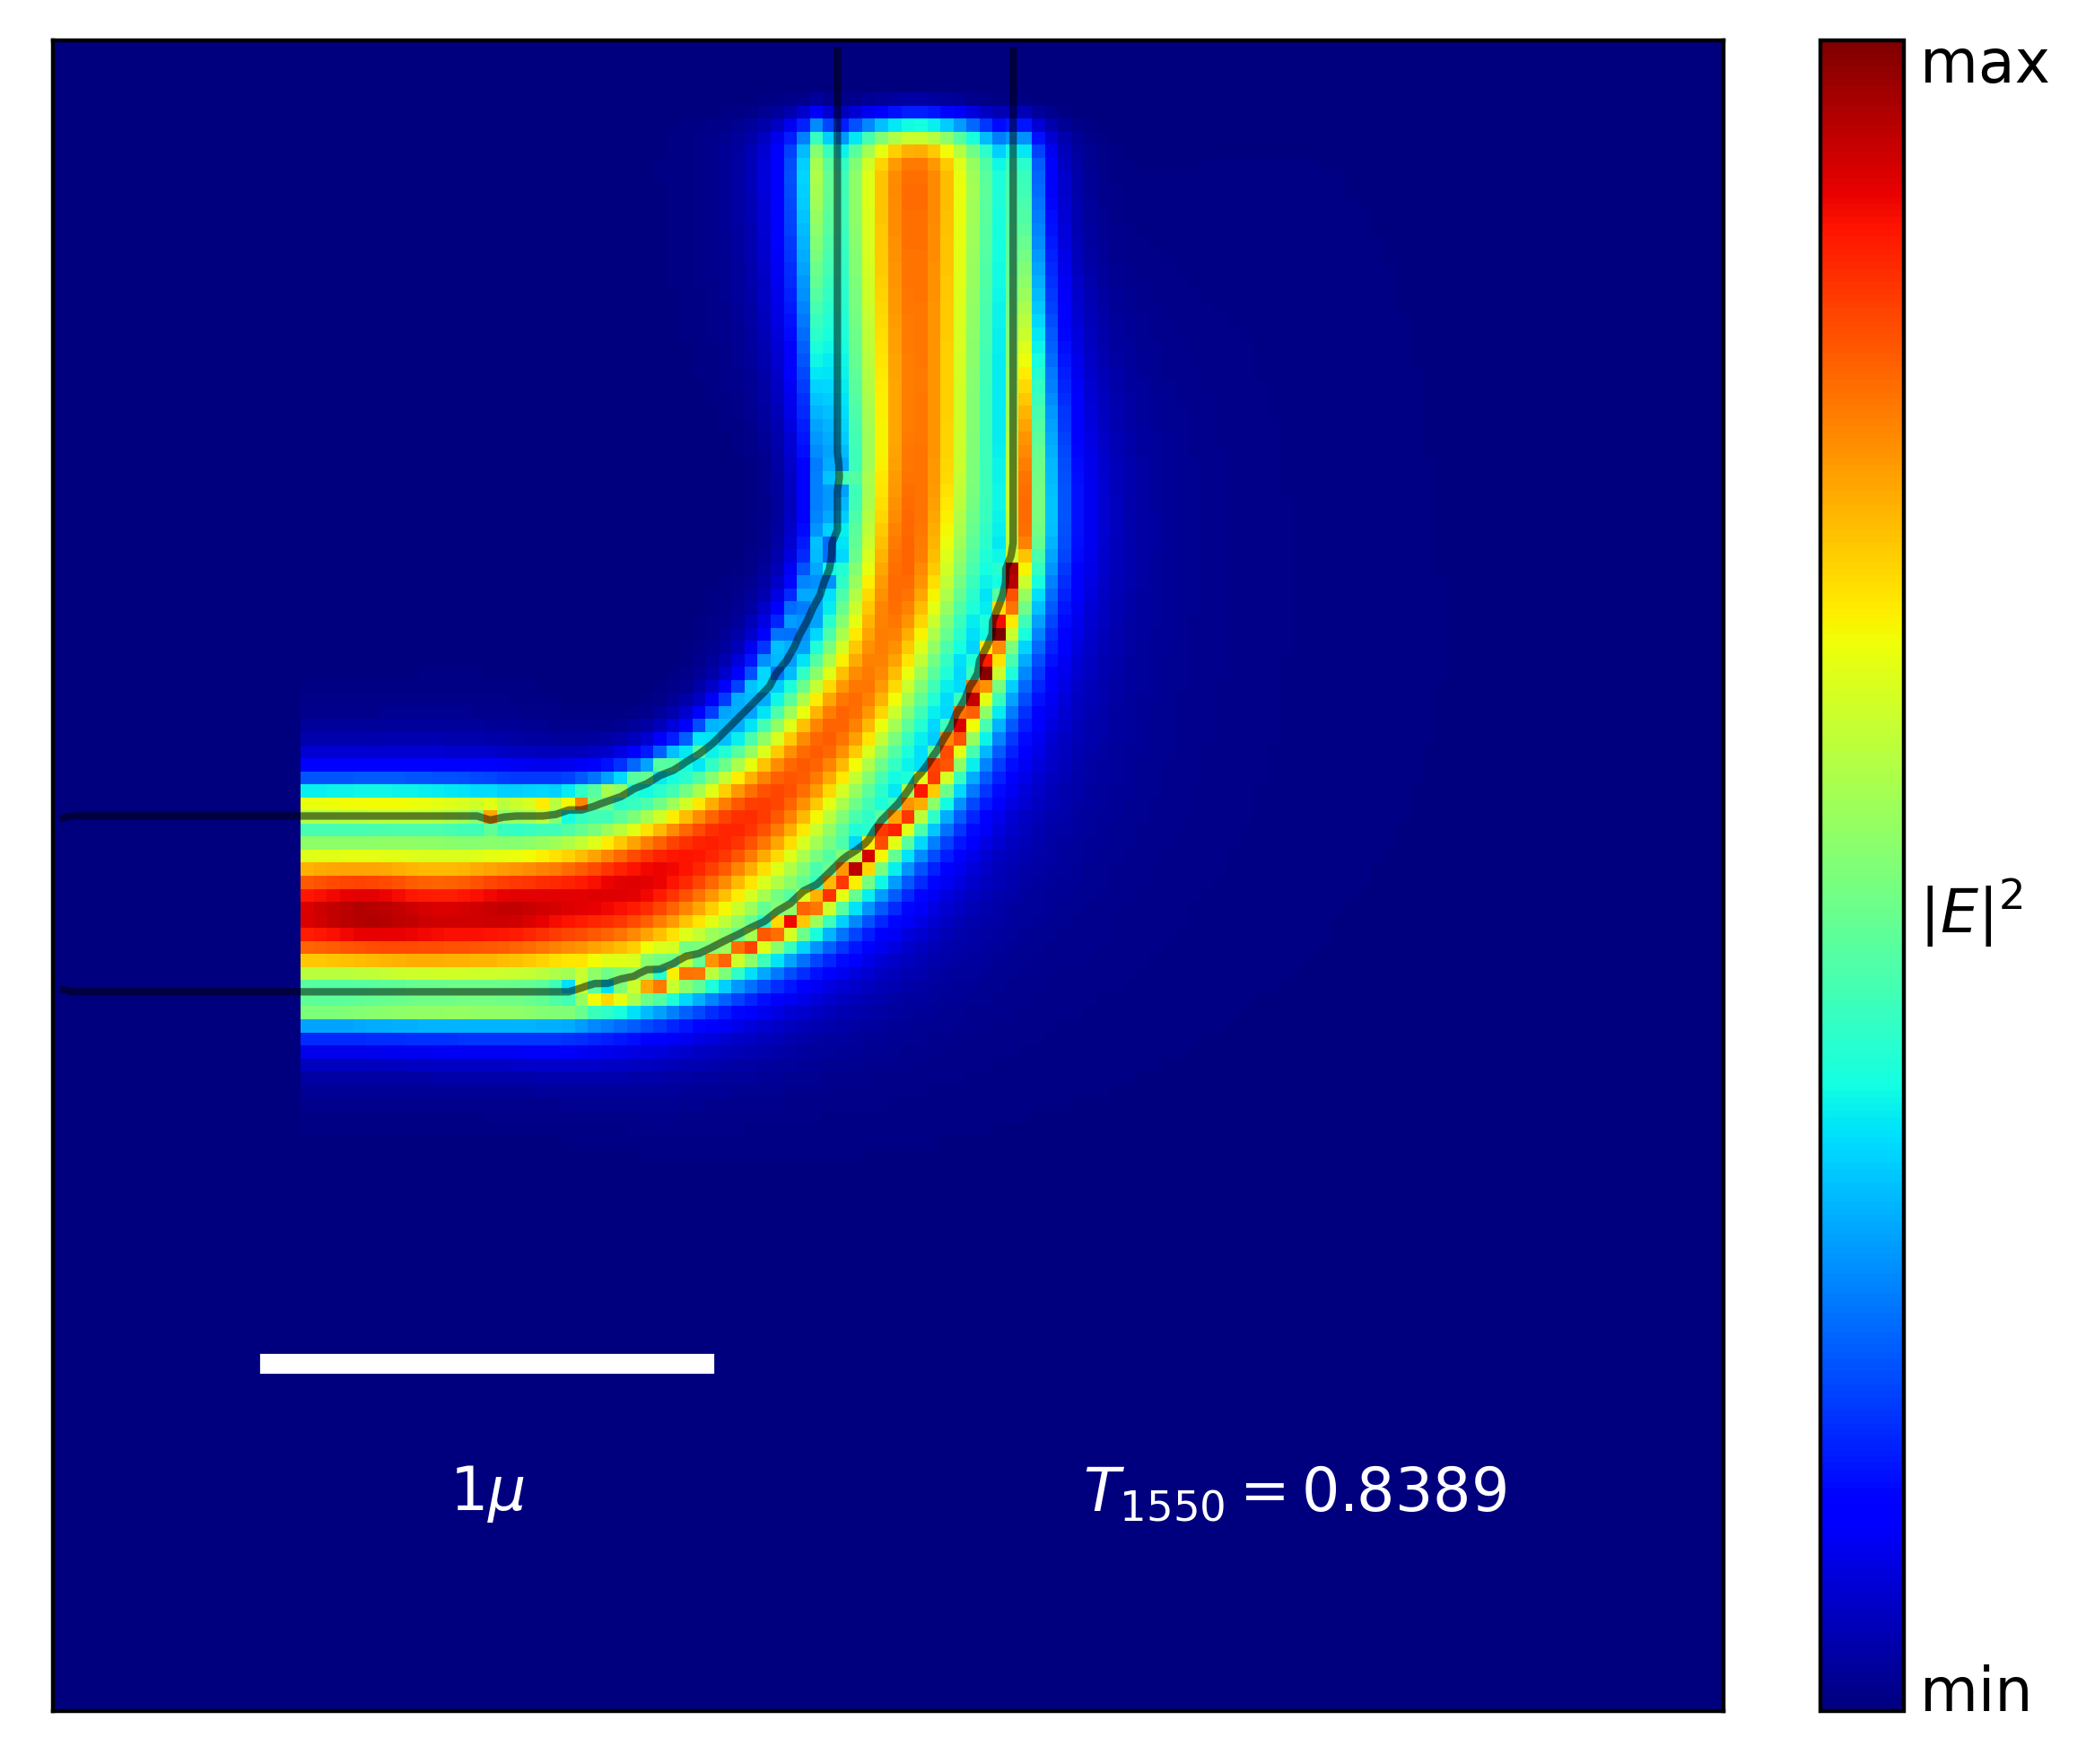
\includegraphics[scale=0.7]{image/theory/bend_field_dx30_px16_rint1000.png}
   \caption{Representación de $|\boldsymbol{E}|^2$ de un \emph{bend} de $1 \mu m$ de radio obtenido usando 3D FDFD bajo una resolución de $30 nm$ en una longitud de onda $\lambda = 1550 nm$.}
  \label{fig:efield}
\end{figure}

Para evitar ambigüedades, dos puntos adicionales a remarcar son: 
(i) cuando nos referimos al radio estamos haciendo mención al radio medio de curvatura y 
(ii) todos los diseños mostrados en este trabajo tienen un profundidad de 220nm.

%Observar en una gráfica el valor de $|\boldsymbol{E}|^2$ nos ayuda a %entender el funcionamiento de un dispositivo.
%Por otro lado, una manera de cuantificar que tan bien funciona un %diseño es mediante el cálculo de la
%transmitancia $(T)$.
%Este valor se define como la relación entre la potencia del flujo que %sale del dispositivo con la 
%potencia del flujo que ingresa \citep{Christiansen2021}.

Seguidamente, sea $\lambda$ la longitud de onda de la entrada y $\boldsymbol{P}$ los parámetros que caracterizan al
diseño, denotaremos como $T_{\lambda}(\boldsymbol{P})$ a la transmitancia asociada al dispositivo obtenido con la
parametrización $\boldsymbol{P}$ en la longitud de onda $\lambda$. Luego, definimos la función objetivo 
($f_{obj}$) para un \emph{bend}, también conocido en el área como figura de mérito (FOM, por sus siglas en
Inglés), 
mediante la siguiente ecuación \citep{Su2020}:

\begin{equation}
  f_{obj}(\boldsymbol{P}) = max \left \{ T_{1550} (\boldsymbol{P}) \right \}.
\label{eq:fom-bend}
\end{equation}

En síntesis, la idea detrás de estas definiciones es describir un \emph{bend} mediante una parametrización
$\boldsymbol{P}$
(\autoref{sec:parametrization}).
Luego, usando algoritmos de optimización, buscar entre las distintas combinaciones de los parámetros aquella configuración
que optimice la función $f_{obj}$ (\autoref{sec:alg-opt}).
De este modo, estaremos encontrando un diseño con una elevada transmitancia, es decir con un buen desempeño.

\subsection{\emph{Wavelength Demultiplexer} (WDM)}

Un WDM es un dispositivo fotónico que se encarga de guiar un haz de ondas de acuerdo a su longitud de onda.
Por ejemplo, estos pueden trabajar con dos longitudes de onda y guían las de una longitud por la guía de onda superior
y las de otra longitud por la guía de onda inferior.

Análogo al caso del \emph{bend}, utilizaremos la transmitancia para cuantificar el desempeño del dispositivo.
Pero, en el presente trabajo usaremos un WDM con dos guías de salida, por ello, utilizaremos como notación
$T_{\lambda}^{(1)}(\boldsymbol{P})$ para
representar la transmitancia en la guía de salida superior cuando se recibe un haz de longitud de onda
$\lambda$ en un diseño descrito por los parámetros $\boldsymbol{P}$ y $T_{\lambda}^{(2)}(\boldsymbol{P})$ para la guía de salida inferior.

\begin{figure}[ht]
  \centering
  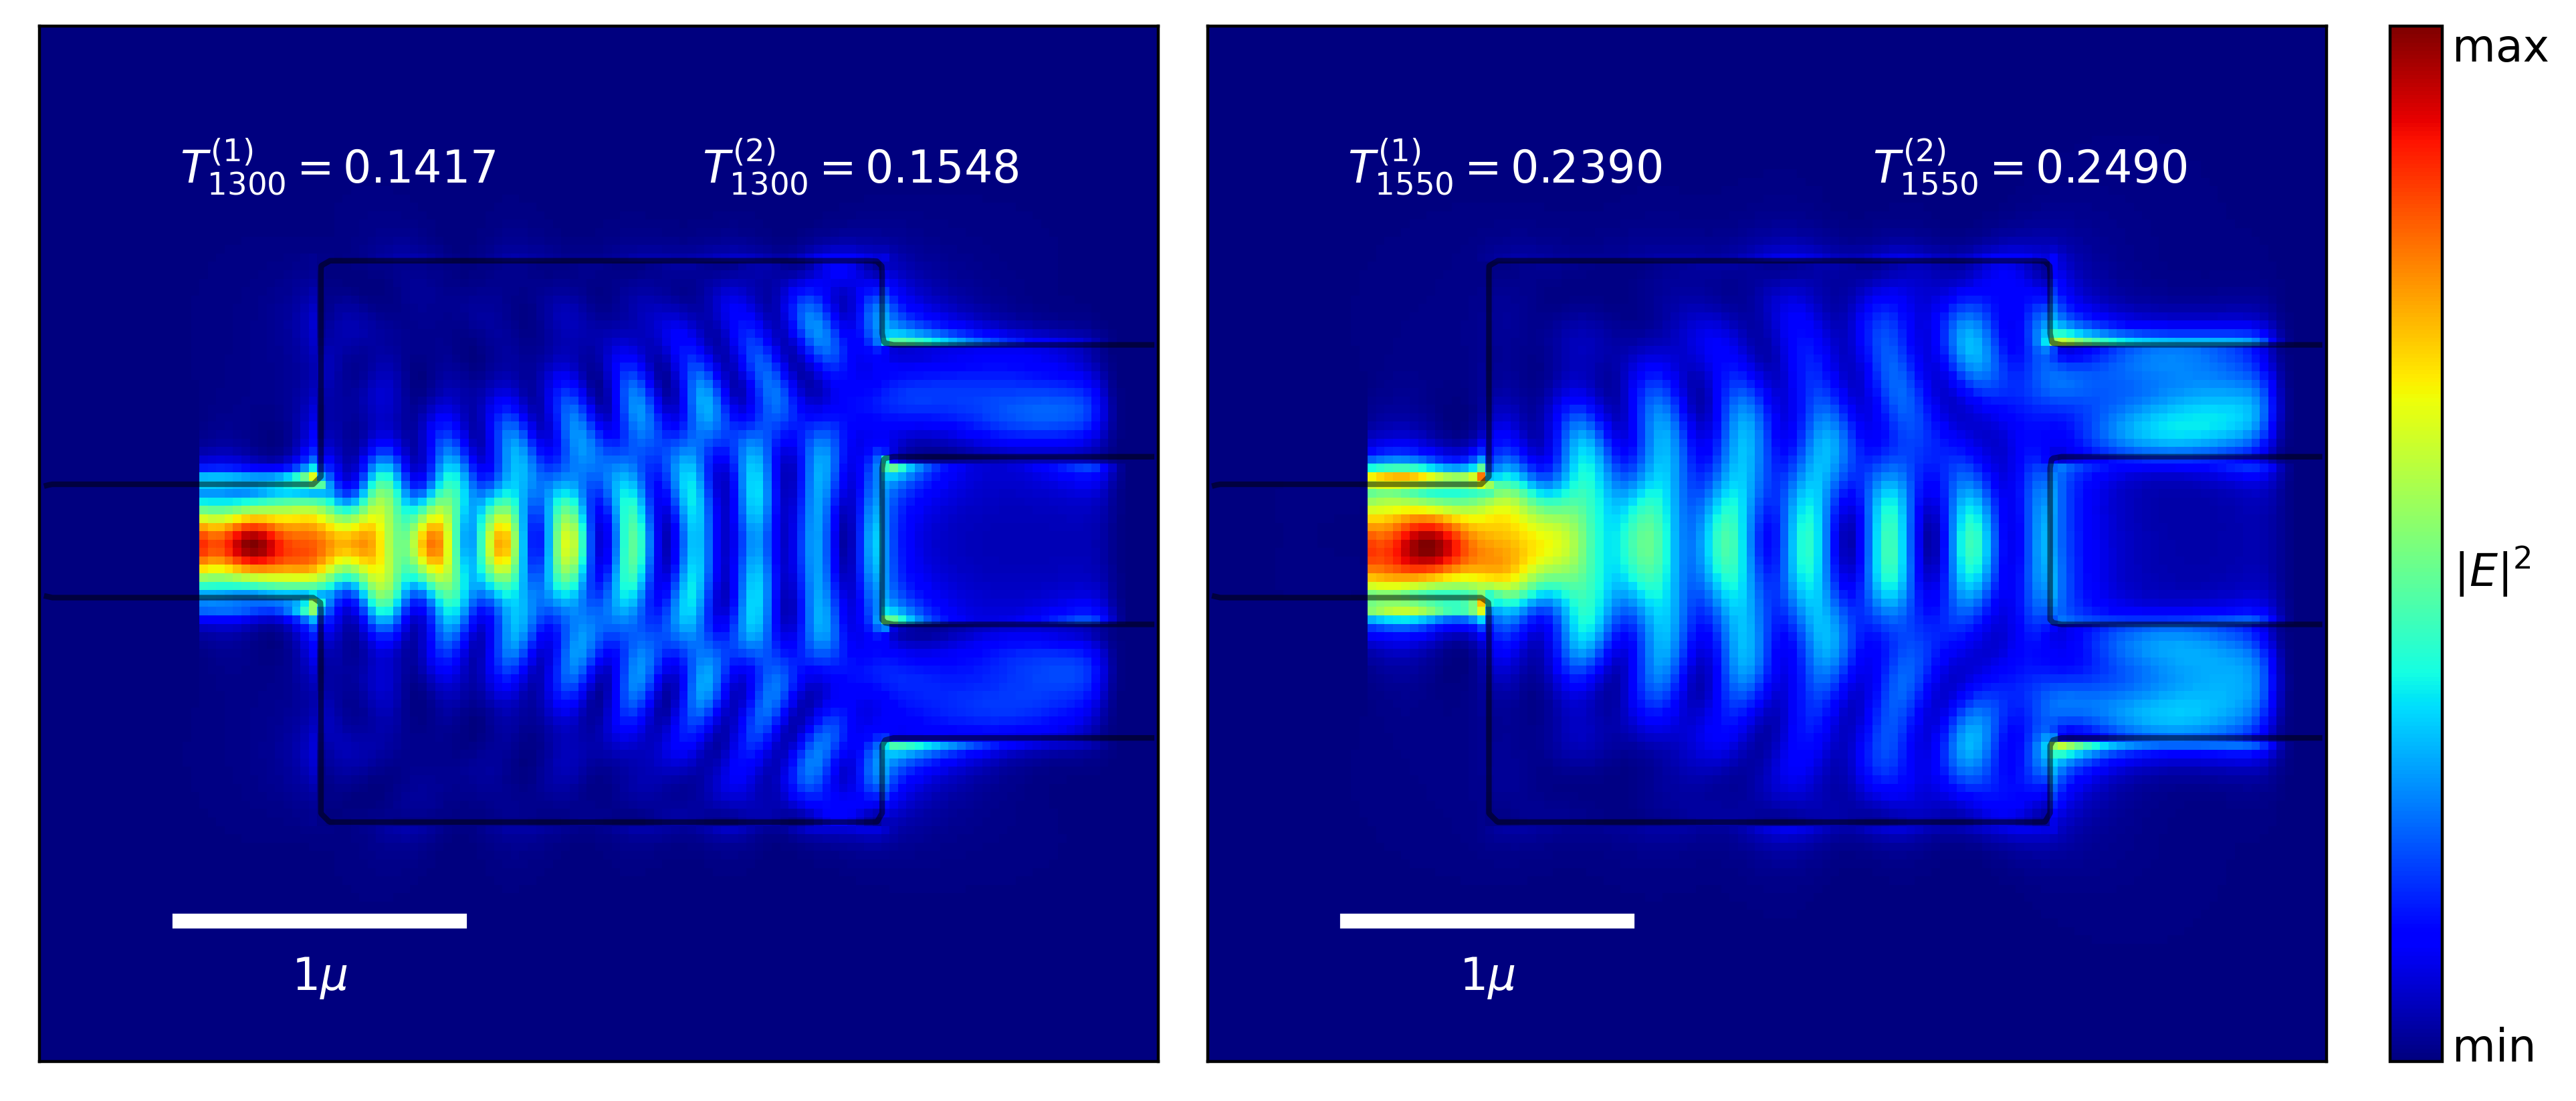
\includegraphics[scale=0.7]{image/theory/wdm_field_dx30_px16_px16.png}
  \caption{Representación de $|\boldsymbol{E}|^2$ de un WDM obtenido usando 3D FDFD bajo una resolución de $30 nm$.}
  \label{fig:efield-wdm}
\end{figure}

En la \autoref{fig:efield-wdm} se muestra un WDM donde las guías de onda son unidas por una región rectangular
de $2.0\mu m \times 2.0 \mu m$. En el lado izquierdo se muestra la representación de $|\boldsymbol{E}|^2$ cuando se usa 
como entrada un haz de ondas de $1300 nm$ de longitud, en el lado derecho la entrada es de $1550 nm$.
En ambos casos el diseño está funcionando más como un \emph{splitter} que como un WDM.
Un \emph{splitter} es un dispositivo fotónico que divide la potencia del flujo de la entrada por las guías
de salida en una determinada proporción. El diseño intuitivo para este dispositivo es el presentado en la imagen. Similar al caso del
\emph{bend}, con unas dimensiones un poco más grandes se puede conseguir pérdidas casi nulas de energía
\citep{LukasChrostowski2010}.
Sin embargo, como se observa en los valores de la transmitancia, este diseño intuitivo no es apropiado para un WDM.

Basándonos en \cite{Su2020}, definimos su FOM como

\begin{equation}
  f_{obj}(\boldsymbol{P}) = max \left \{ \frac{\left ( T_{1300}^{(1)}(\boldsymbol{P}) \right )^2  + 
                            \left ( 1 - T_{1300}^{(2)}(\boldsymbol{P}) \right )^2 +
                            \left ( 1 - T_{1550}^{(1)}(\boldsymbol{P}) \right )^2  + 
                            \left ( T_{1550}^{(2)}(\boldsymbol{P}) \right )^2 }{4}
                    \right \}.
\label{eq:fom-splitter}
\end{equation}

La \autoref{eq:fom-splitter} busca maximizar la transmitancia por la guía de onda superior y minimizarla para
la guía de onda inferior cuando se recibe una longitud de onda de $1300 nm$ y lo contrario para una longitud
de onda de $1550 nm$. Cabe destacar que la división por cuatro se realiza para asegurar que $f_{obj}$ solamente
tenga valores en el intervalo $[0, 1]$, al igual que sucede con la función objetivo del \emph{bend}.

La idea para optimizar un WDM es la misma descrita en la anterior sección. 
En el resto del capítulo se describe en más detalle los siguientes pasos necesarios para lograr esto.

\section{Parametrización}\label{sec:parametrization}

Tanto para el \emph{bend} como para el WDM se define una región de diseño
mediante una parametrización ($\boldsymbol{P}$) que permita mapear un conjunto amplio de estos dispositivos.
Una de la estrategias más populares para esta tarea es usar parametrización
basada en píxeles. Esta estrategia consiste en definir $\boldsymbol{P}$ como una matriz 
de $n$ filas y $m$ columnas con valores en el intervalo $[0, 1]$.
Al proceso de optimizar un dispositivo con esta parametrización se le conoce como optimización
topológica \citep{Molesky2018}.

\begin{figure}[h]
  \centering
  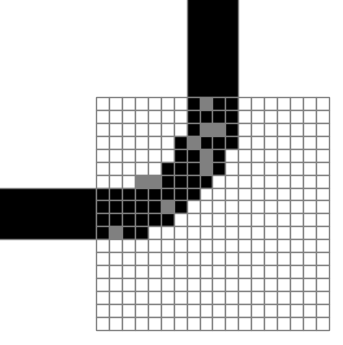
\includegraphics[scale=0.7]{image/theory/parametrization-pixeles.png}
  \caption{Parametrización basada en píxeles para un \emph{bend} definiendo $\boldsymbol{P}$ como una matriz de $18 \times 18$.}
  \label{fig:pixeles}
\end{figure}

A modo de ejemplo, en la \autoref{fig:pixeles} se ha definido la matriz $\boldsymbol{P}: [1, n] \times [1, m]
\to [0, 1]$ con $n = m = 18$ y se ha graficado sus valores
usando escala gris (0 corresponde al color blanco, 1 al negro y los demás valores a diferentes
intensidades del gris). De esta manera observamos como $\boldsymbol{P}$ logra definir la geometría de un
diseño.
Adicionalmente, conforme se incrementa el valor de $n$ y $m$ se logra definir detalles con mayor precisión.


Sin embargo, lo anterior solo nos permite describir la geometría de los diseños, no sus propiedades.
Además, no queda claro qué representan las regiones grises.
Por ello, para describir las propiedades del diseño es necesario asociar a $\boldsymbol{P}$ alguna propiedad física.
Esto lo realizamos calculando la permitividad ($\boldsymbol{\varepsilon}$) mediante la siguiente ecuación:

\begin{equation}
  \boldsymbol{\varepsilon}(x, y) = \varepsilon_{Si} * \boldsymbol{P}(x, y) + (1 - \boldsymbol{P}(x, y))
  \varepsilon_{SiO_2} \, \mid \, x \in [1, n] \land y \in [1, m],
\label{eq:permitivity}
\end{equation}

\noindent donde $\varepsilon_{Si} = 3.48^2$ es la permitividad del silicio ($Si$) y
$\varepsilon_{SiO_2} = 1.44^2$ es la permitividad del óxido de silicio ($SiO_2$).
De esta manera, la celda ubicada en la fila $x$, columna $y$ de la geometría descrita por 
$\boldsymbol{P}(x, y)$ tiene una permitividad de valor $\boldsymbol{\varepsilon}$(x, y).

Con la \autoref{eq:permitivity} estamos asociando a cada rectángulo de la geometría descrita por
$\boldsymbol{P}$ un valor de permitividad en el rango 
$[\varepsilon_{SiO2} = 1.44^2, 3.48^2 = \varepsilon_{Si}]$.
De esta manera, $\boldsymbol{P}(x, y) = 1$ describe que el rectángulo ubicado en la posición $(x, y)$ es de
$Si$,
un valor de $\boldsymbol{P}(x, y) = 0$ describe la presencia de $SiO_2$ y 
$0 < \boldsymbol{P}(x, y) < 1$ hace referencia
a algún material cuya permitividad es $\boldsymbol{\varepsilon}(x, y)$.

Nótese que un inconveniente de lo descrito es que $\boldsymbol{P}$ puede mapear a materiales inexistentes
(regiones grises),
mayor detalle de esta dificultad se estudia
en la \autoref{sec:transformations}.
Por otro lado, con la descripción de la permitividad podemos calcular los campos eléctricos con los
cuales se puede obtener el valor de $f_{obj}$ definido para el \emph{bend} y WDM.
Por esta razón se realizan simulaciones electromagnéticas y se resuelven las inversas de las 
ecuaciones de Maxwell, esto permite obtener los campos eléctricos \citep{Su2020}.
%Afortunadamente, para este proceso se puede utilizar distintos programas que implementan diversos 
Para este proceso se pueden utilizar distintos programas que implementan diversos
métodos numéricos para realizar los cálculos (\autoref{sec:simulation}).

\section{Simulación}\label{sec:simulation}

Una vez tenemos definido un dispositivo con regiones fijas (guías de onda) y una
región de diseño descrita por la parametrización, es necesario incorporar
tres componentes adicionales \citep{Oskooi2010, Su2020}:

\begin{enumerate}

  \item \textbf{Fuente:} Suele representarse como un rectángulo en un plano perpendicular al flujo
    que pasa por el lugar donde este se ubica. Simula la emisión de un haz de ondas por el diseño.

  \item \textbf{Monitores:} Suelen representarse como un rectángulo similar a la fuente.
    Capturan información en su ubicación, en nuestro estudio valores del campo eléctrico.

  \item \textbf{\emph{Perfectly Matched Layer} (PML):} Representan las condiciones de frontera en la simulación. 
    Se utilizan para limitar el espacio donde se deberá realizar las simulaciones computacionales.

\end{enumerate}

\begin{figure}[ht]
  \centering
  \subfigure[Vista longitudinal del dominio computacional.]
    {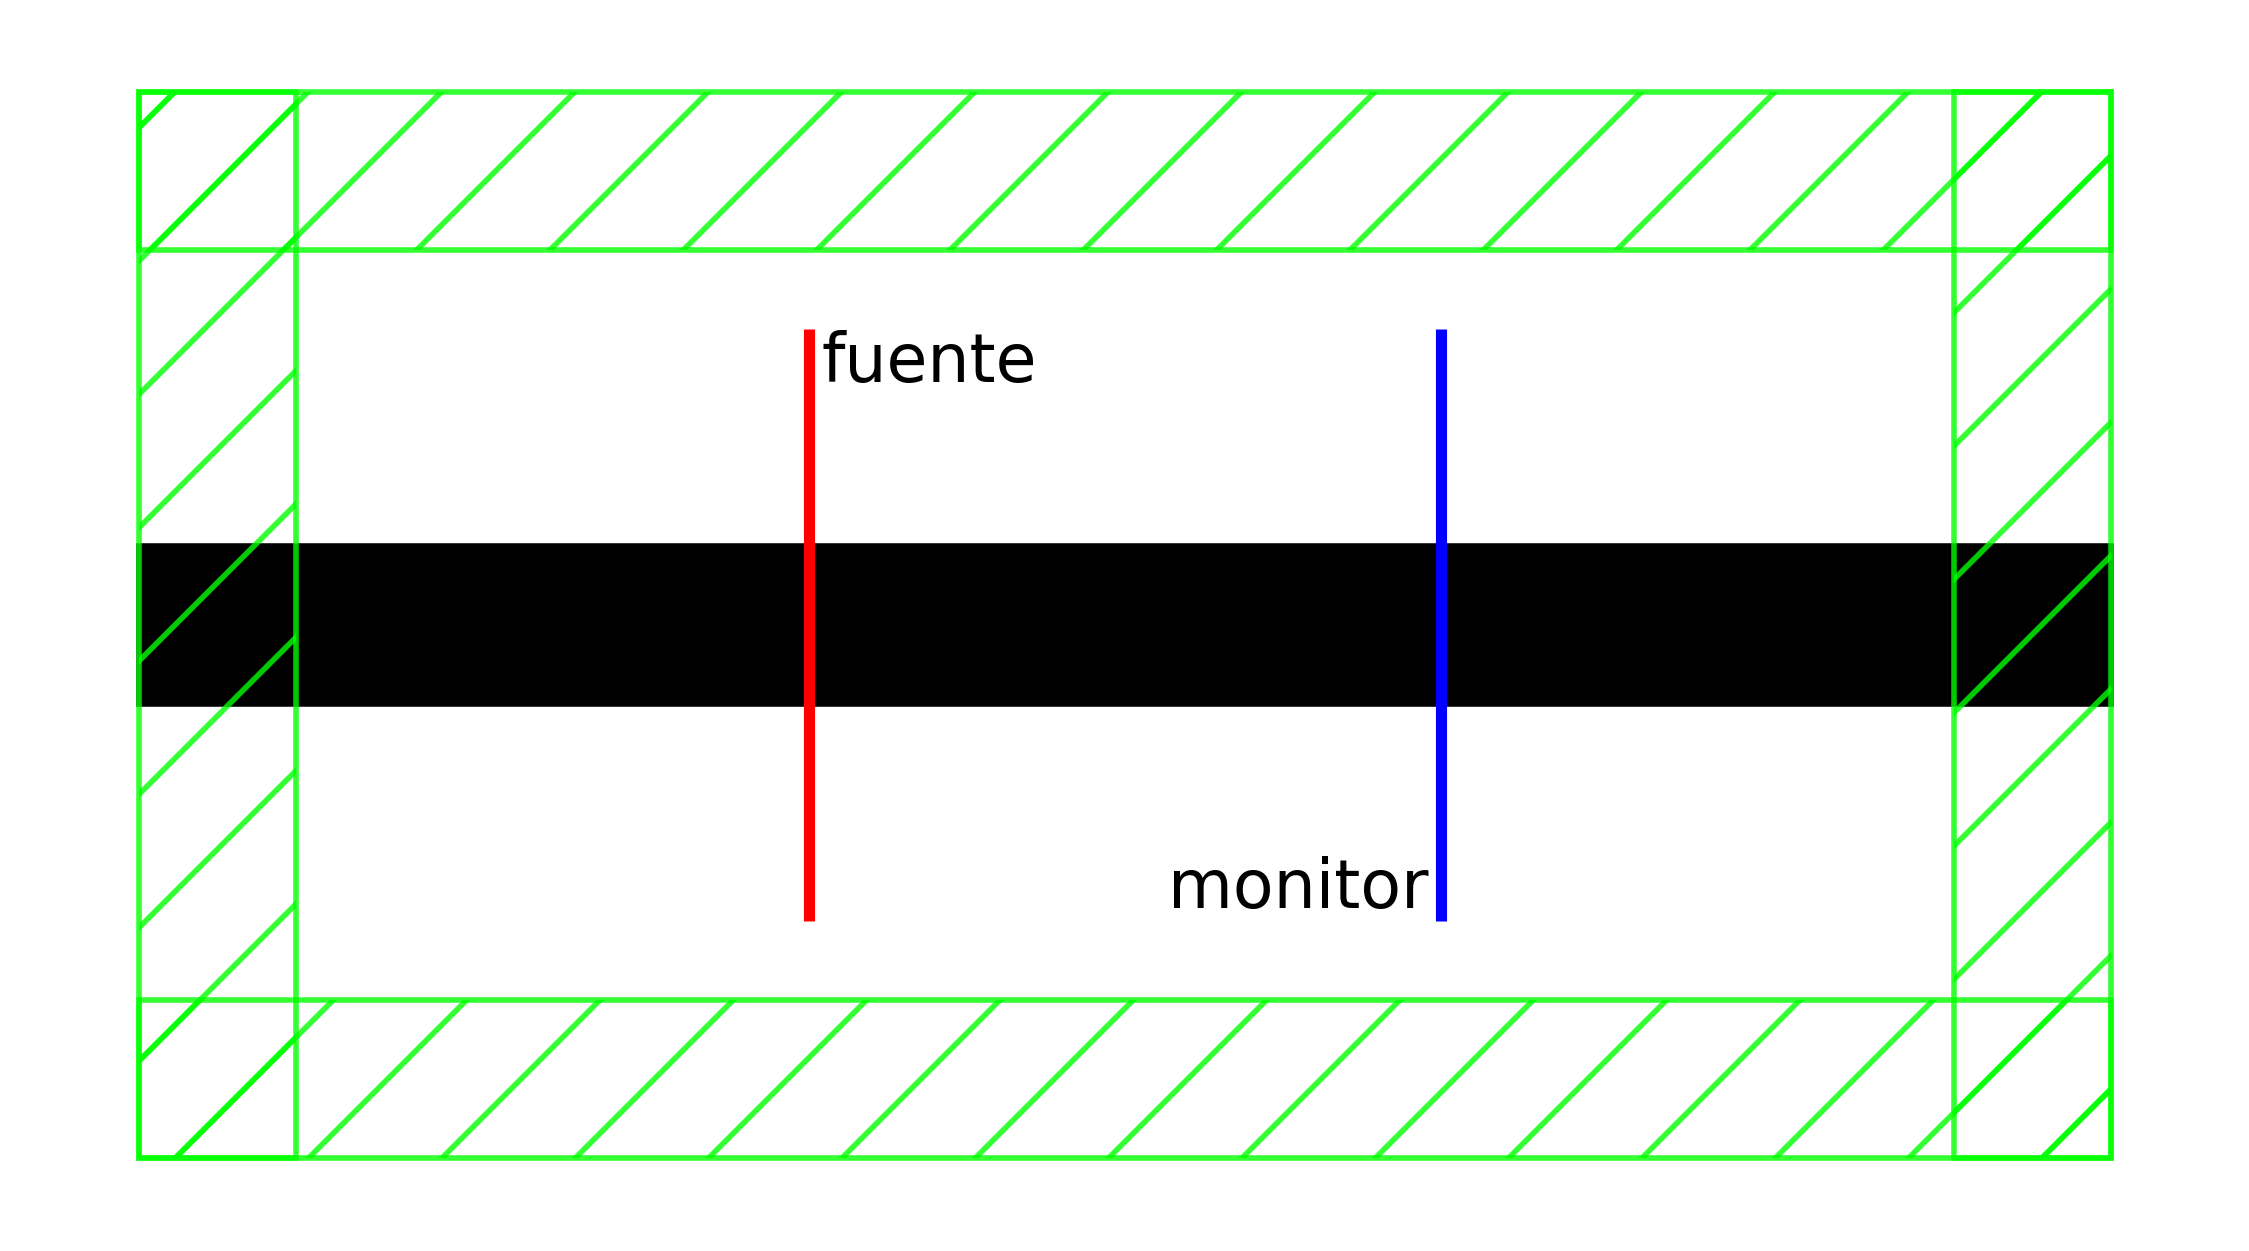
\includegraphics[width=0.45\textwidth]{image/theory/simulation.png}\label{fig:waveguide-a}}
  \hfill
  \centering
  \subfigure[Vista transversal de la fuente de la guía de onda.]
    {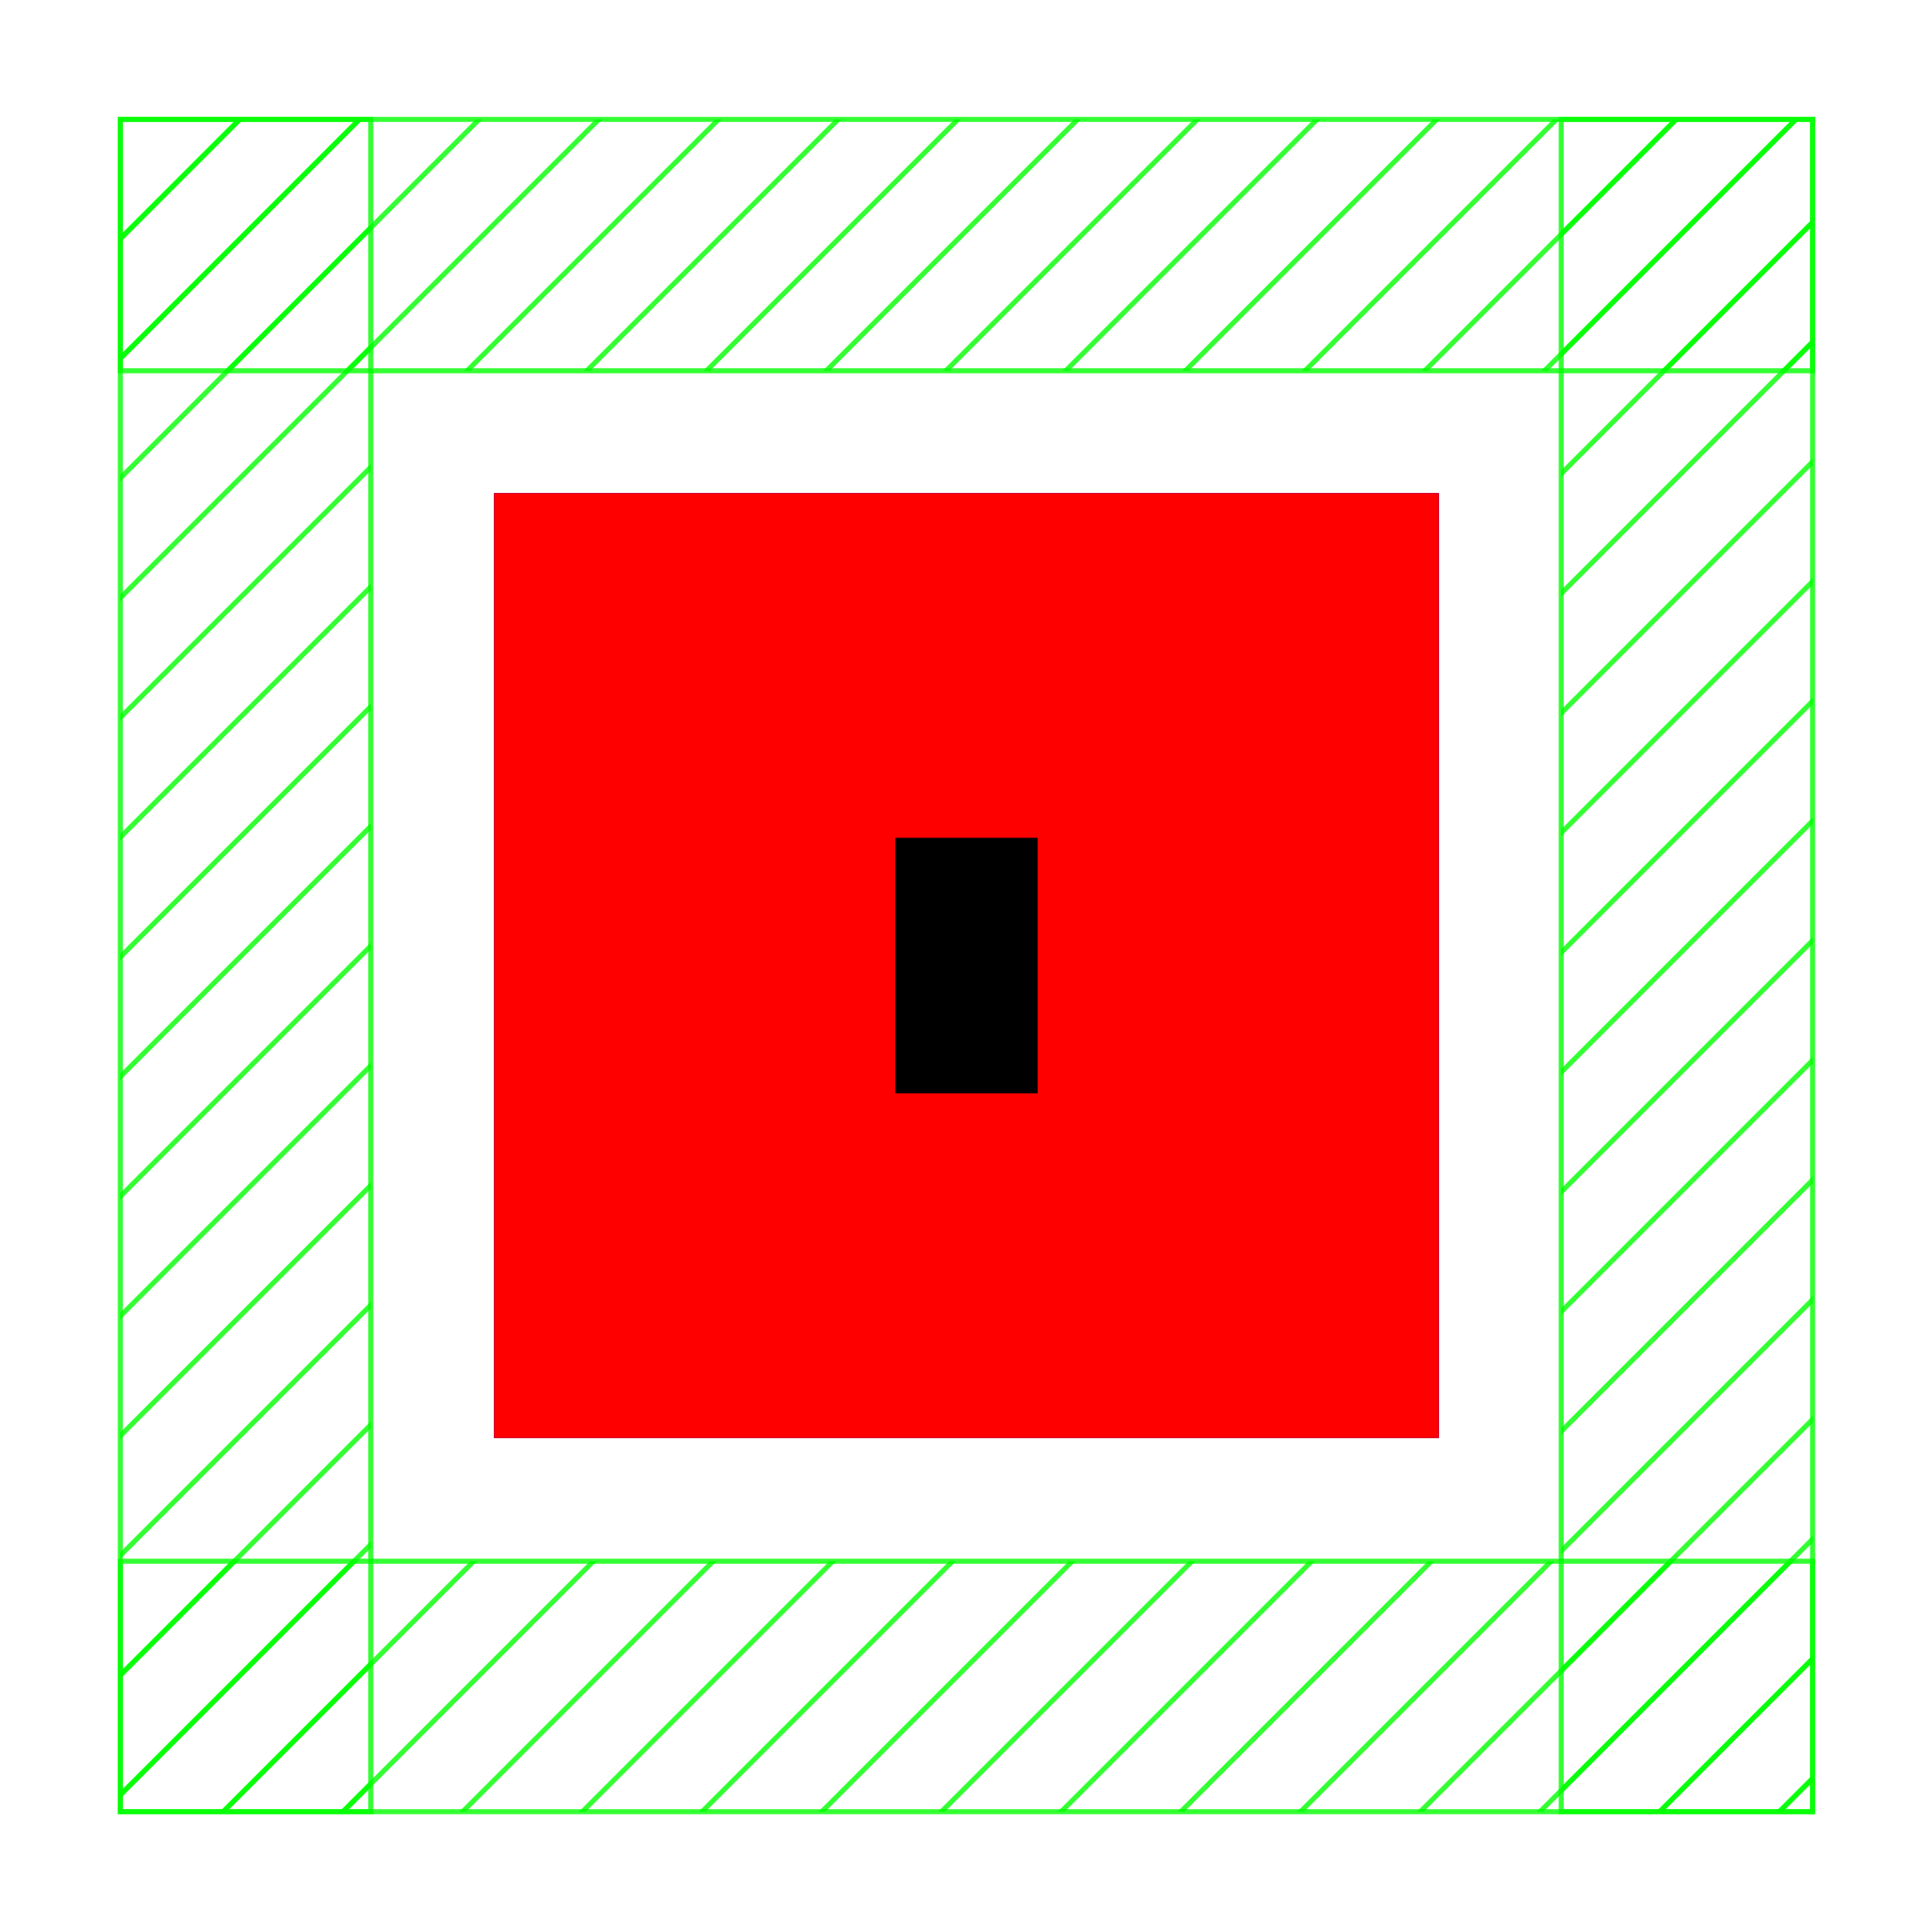
\includegraphics[width=0.45\textwidth]{image/theory/simulation-left.png}\label{fig:waveguide-b}}

  \centering
  \subfigure[Vista transversal del monitor de la guía de onda.]
    {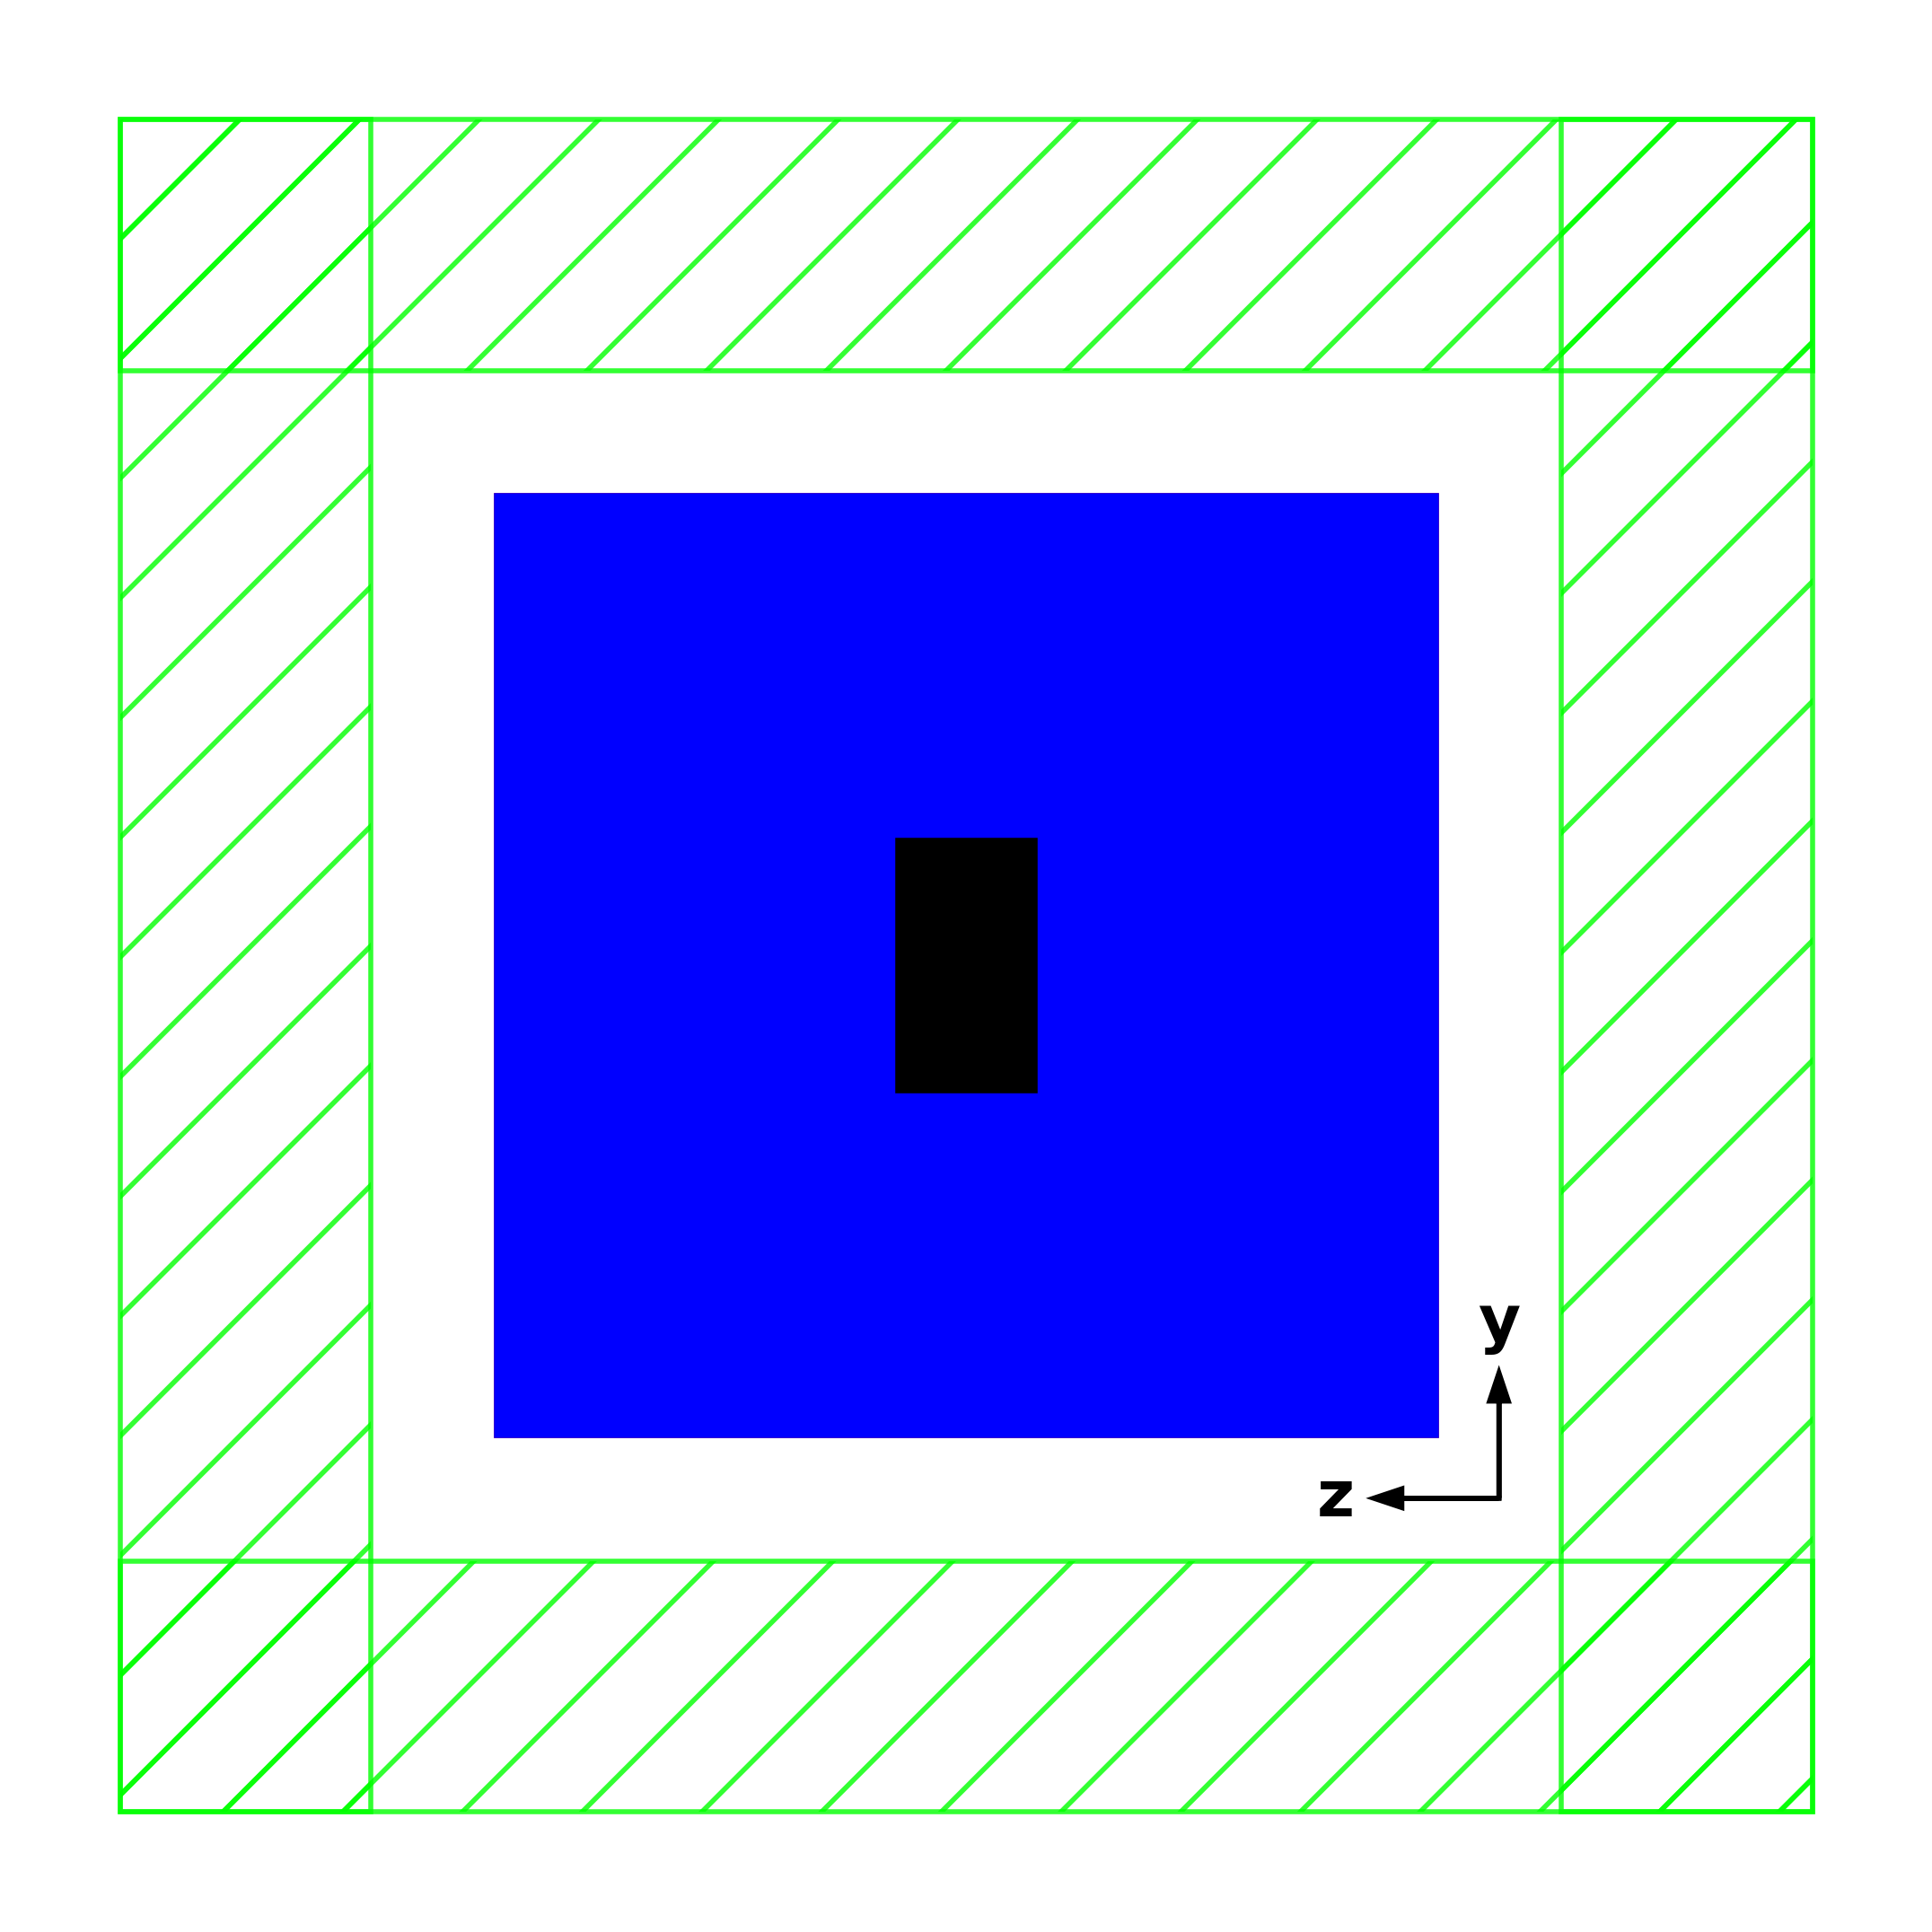
\includegraphics[width=0.45\textwidth]{image/theory/simulation-right.png}\label{fig:waveguide-c}}
  \hfill
  \centering
  \subfigure[Análisis modal de una guía de onda de 400nm simulado con SPINS-B usando una resolución de 10nm.]
    {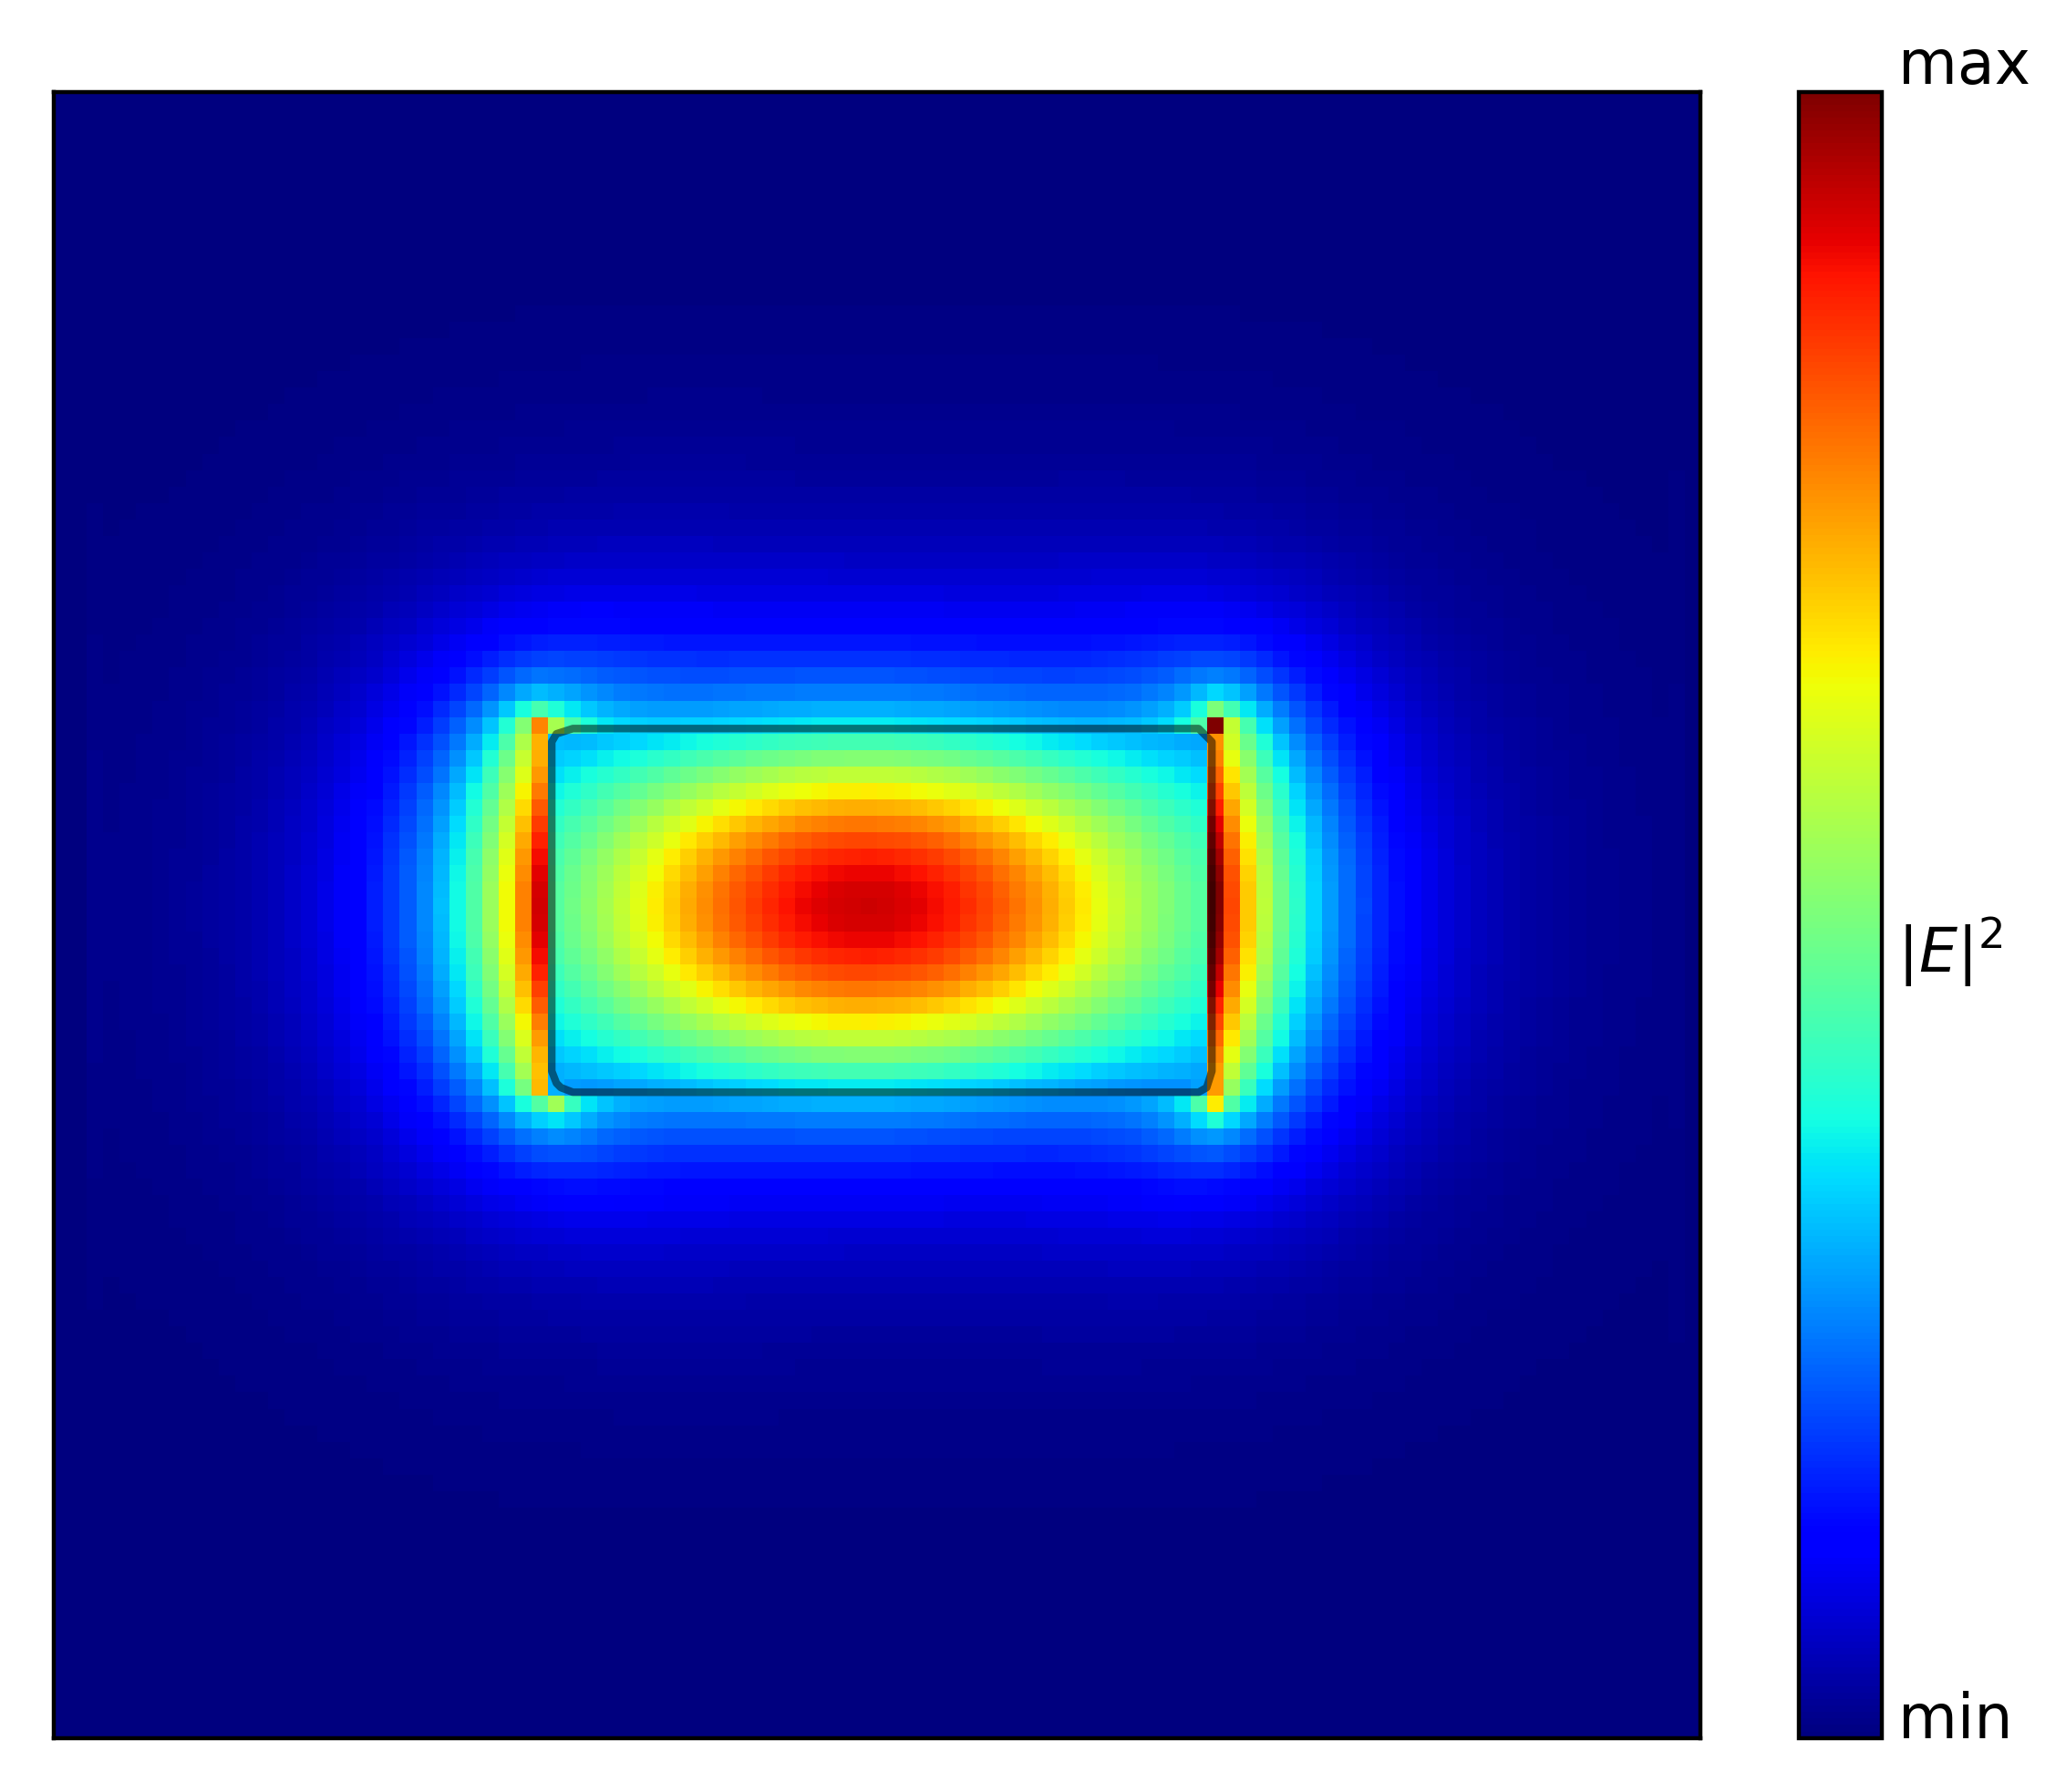
\includegraphics[width=0.45\textwidth]{image/theory/simulation-modal.png}\label{fig:waveguide-d}}

  \caption{Configuración de simulación para una guía de onda en 3D.}
  \label{fig:waveguide}
\end{figure}

La \autoref{fig:waveguide} ilustra una guía de onda en 3D con las tres componentes anteriores.
El rectángulo de color negro representa la guía de onda, la región roja la fuente, 
la región azul el monitor y lo verde el PML.
Guiándonos de la Figura \autoref{fig:waveguide-a}, al realizar una simulación con esta configuración 
el flujo iría de la región roja a la región azul. Este seguiría expandiéndose por la guía de onda hasta llegar a la región verde (PML).
En palabras sencillas, podemos interpretar el PML como una caja que permite aislar nuestro sistema. 
Pero, es importante que el PML se superponga con el dispositivo para evitar errores numéricos.
Por otro lado, la Figura \autoref{fig:waveguide-b} representa el mismo diseño pero desde una vista transversal
(recordemos que son diseños en 3D) y lo mismo ocurre en la Figura \autoref{fig:waveguide-c}, pero esta es una
vista transversal desde otro ángulo.
Con la ayuda de las vistas transversales se evidencia como la fuente y el monitor son representados por
rectángulos, no por rectas. Por último, en la Figura \autoref{fig:waveguide-d} se muestra la distribución
del campo eléctrico del modo TE calculado en la fuente y medido en el monitor. Notemos que para los distintos
cálculos solo necesitaremos los valores asociados al modo TE.

Siguiendo lo descrito, podemos utilizar diversos programas para configurar y ejecutar 
simulaciones de un \emph{bend} y WDM.
Una alternativa es usar SPINS-B junto a Maxwell-B, programas implementados en Python como código abierto.
Estos funcionan bajo una arquitectura cliente-servidor donde SPINS-B es el cliente y Maxwell-B es el servidor.

Por un lado, SPINS-B permite configurar diseños (fuente, monitores, PML, parametrización, región de diseño, etc.) y solicitar al servidor que obtenga sus propiedades.
Un aspecto interesante de este simulador es que trabaja con bloques llamados nodos.
Estos representan operaciones fundamentales como suma, resta, multiplicación, etc.
Luego, el programa guarda nuestra función objetivo ($f_{obj}$) usando un grafo que tiene estos nodos de vértices.
Así, SPINS-B permite calcular de forma eficiente
(usando un número de simulaciones independiente de las dimensiones de $\boldsymbol{P}$) 
el valor de $\nabla f_{obj}(\boldsymbol{P})$ mediante diferenciación automática \citep{Su2020, Mykel2019}.

Por otro lado, Maxwell-B es un \emph{solver} que implementa un método numérico conocido como \emph{finite-difference frequency domain}
(FDFD) para resolver numéricamente las ecuaciones de Maxwell y obtener así determinadas propiedades
de los diseños que recibe.
Es importante destacar que la implementación de esta librería es en GPUs de NVIDIA y permite
aprovechar múltiples GPUs a la vez.


Un último detalle a señalar es que para las simulaciones debemos definir su resolución,
esto lo representamos con el parámetro $dx$. 
Su valor se utiliza para discretizar nuestro espacio de
simulación en una malla de cubos de dimensiones $dx \times dx \times dx$.
En general, cuanto más pequeño es este valor
los resultados son más precisos, pero la cantidad de memoria y el tiempo de
simulación se incrementan considerablemente.

\section{Transformaciones}\label{sec:transformations}

En esta sección se discute dos transformaciones populares en optimización topológica
para imponer restricciones de fabricación en nuestros diseños: (i) filtro por densidad y
(ii) proyección.
Esta sección está basada en \cite{Lazarov2016}, para una descripción más detallada revisar este trabajo.

\subsection{Filtro por Densidad}

Antes de definir el filtro por densidad, necesitamos definir el concepto de bola cerrada.
Para ello, tenemos que definir el concepto de función distancia en nuestra matriz
de parametrización. Así, sea $x, x' \in [1, n] \land y, y' \in [1, m]$, definimos 
la distancia entre las posiciones $(x, y)$ y $(x', y')$ de la matriz $\boldsymbol{P}$ como:

\begin{equation}
  dis(x, y, x', y') = |x-x'|*psize_y+|y-y'|*psize_x,
  \label{eq:distance}
\end{equation}

\noindent donde $psize_x$ es el valor de la longitud horizontal que representa cada celda de $\boldsymbol{P}$
y $psize_y$ es el recíproco para la longitud vertical. \leonidas{Notemos que esta función distancia se comporta
como la distancia de Manhattan, pero aplicando pesos.}

De esta manera, definimos la bola cerrada ($\overline{B}_{r}(x, y)$)  de centro $(x, y)$ y 
radio $0 < r$ mediante el siguiente conjunto:

\begin{equation}
  \overline{B}_{r}(x, y) = \{(x', y') | 1 \leq x' \leq n \land 1 \leq m \leq m \land 
  dis(x, y, x', y') \leq r\}.
  \label{eq:bola}
\end{equation}

Seguidamente, usando estos conceptos en la matriz $\boldsymbol{P}$
se define el filtro por densidad ($\widetilde{\boldsymbol{P}}$) mediante la ecuación:

\begin{equation}
  \widetilde{\boldsymbol{P}}(x, y) = \frac{\displaystyle\sum_{(x', y') \in \overline{B}_{r_f}(x, y)} w_{x, y}(x', y')
  A(x', y')\boldsymbol{P}(x', y')}
  {\displaystyle\sum_{(x', y') \in \overline{B}_{r_f}(x, y)} w_{x, y}(x', y') A(x', y')},
  \label{eq:densityfilter}
\end{equation}

\begin{equation}
  w_{x, y}(x', y') = max(0, r_f - dis(x, y, x', y')),
  \label{eq:hatbased}
\end{equation}

\noindent donde $A(x, y)$ es el área de la celda representada por $\boldsymbol{P}(x, y)$. 
Por otro lado, el concepto de mínimo radio de curvatura ($r_f$) hace referencia a que un diseño
se puede dibujar con una circunferencia de radio $r_f$.
El objetivo de la \autoref{eq:hatbased} es tratar de imponer este concepto al diseño.

Finalmente, de la \autoref{eq:densityfilter} podemos obtener el valor de su derivada parcial respecto al diseño
original calculando lo siguiente:

\begin{equation}
  \frac{\partial\widetilde{\boldsymbol{P}}(x, y)}{\partial \boldsymbol{P}(x^{*}, y^{*})} = \frac{w_{x, y}(x^{*},
  y^{*})A(x^{*}, y^{*})}
  {\displaystyle\sum_{(x', y') \in \overline{B}_{r_f}(x, y)} w_{x, y}(x', y') A(x', y')}.
  \label{eq:densityfiltergrad}
\end{equation}

\subsection{Proyección}

La proyección descrita en la sección anterior ayuda a obtener diseños que eviten regiones puntiagudas;
sin embargo, esta transformación suele generar regiones grises.
Por este motivo, es común acompañar el filtro por densidad con una proyección 
($\widetilde{\widetilde{\boldsymbol{P}}}$) descrita como:

\begin{equation}
  \widetilde{\widetilde{\boldsymbol{P}}}(x, y) = \frac{\tanh (\beta \times \eta) + \tanh (\beta \times
  (\widetilde{\boldsymbol{P}}(x, y)
  - \eta))}{\tanh (\beta \times \eta) + \tanh (\beta \times (1 - \eta))},
  \label{eq:projection}
\end{equation}

\noindent donde $\eta$ y $\beta$ son números escalares. Para entender el impacto de estos parámetros
en la \autoref{eq:projection}, veamos la \autoref{fig:discretization}.
En la figura graficamos esta ecuación con un valor fijo de $\eta = 0.5$ y distintos valores de
$\beta$.
Se observa que con $\beta = 1$ tenemos prácticamente la función identidad y conforme aumenta
el valor de $\beta$ la función se aproxima más a una función escalonada con quiebre en $0.5$. 
En general el quiebre se realiza en el valor que se le de a $\eta$.

    \begin{figure}[ht]
      \centering
      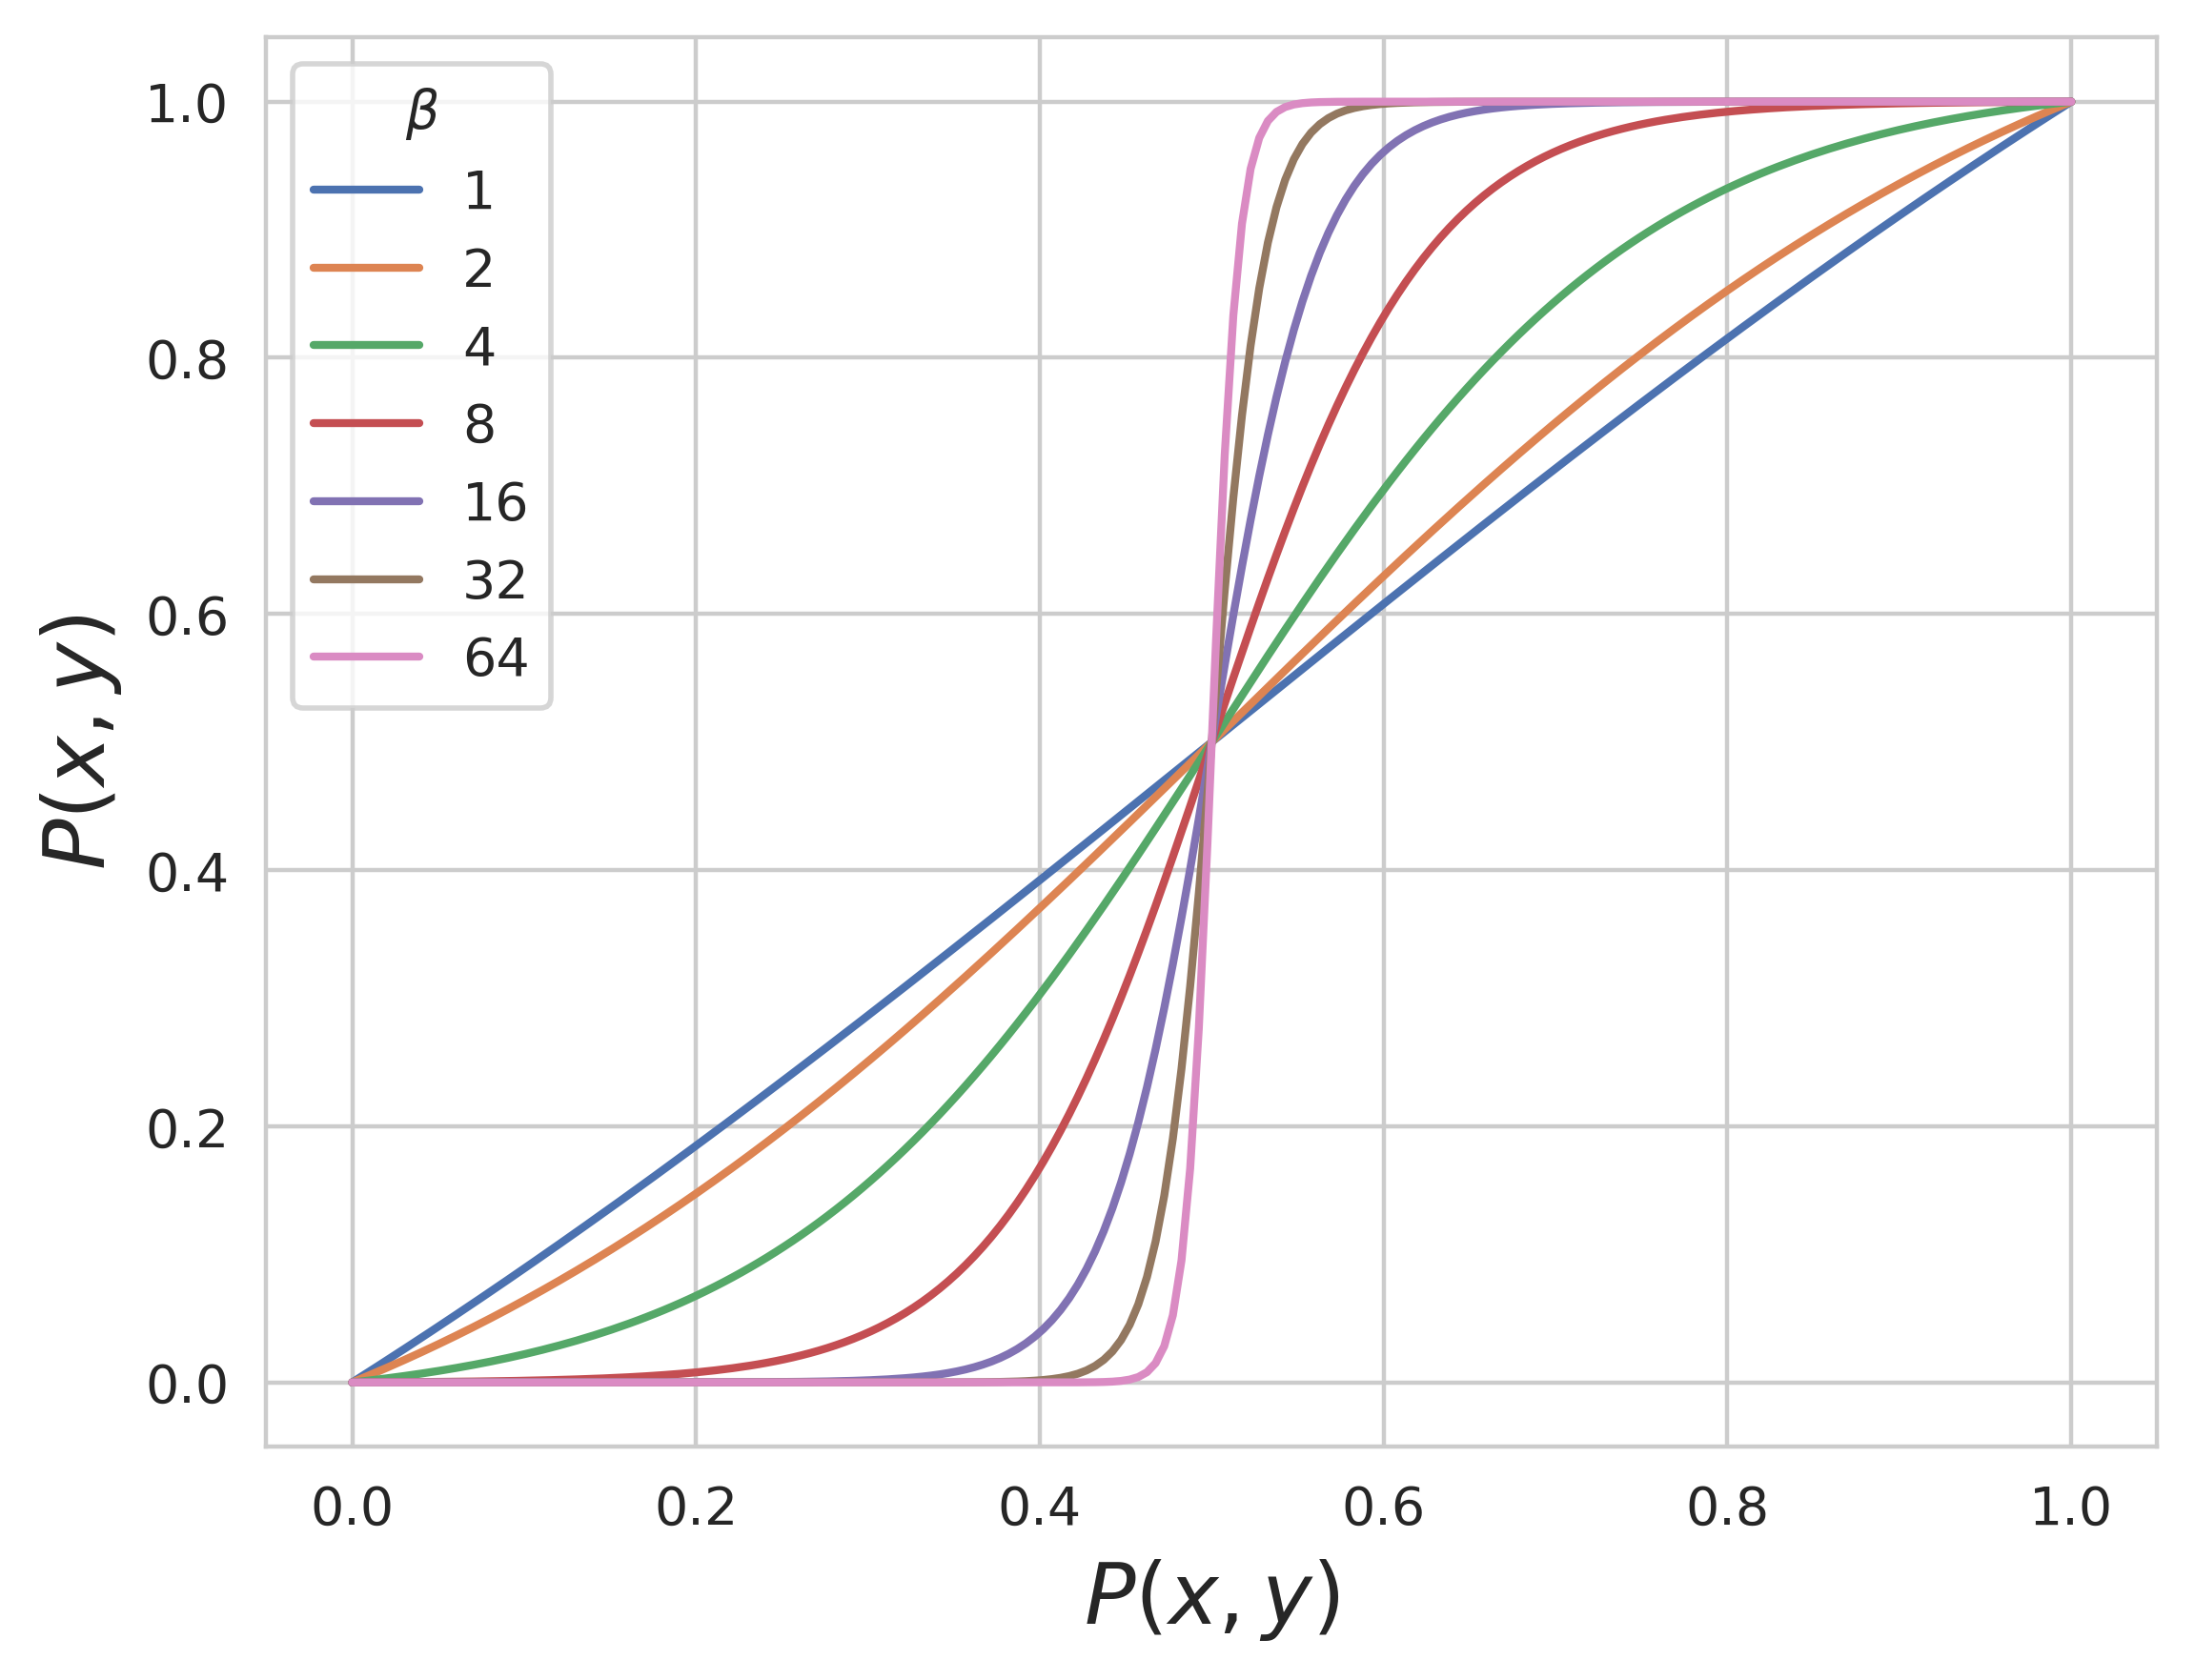
\includegraphics[scale=0.75]{image/theory/discretization.png}
      \caption{Transformación de proyección con $\eta = 0.5$ y distintos valores
      de $\beta$.}
      \label{fig:discretization}
    \end{figure}

Además, de la \autoref{eq:projection} podemos obtener el valor de su derivada parcial 
respecto al diseño $\widetilde{\boldsymbol{P}}$ mediante la siguiente ecuación:

\begin{equation}
  \frac{\partial\widetilde{\widetilde{\boldsymbol{P}}}(x, y)}{\partial \widetilde{\boldsymbol{P}}(x, y)} =
  \frac{(1 - \tanh^2 (\beta \times (\widetilde{\boldsymbol{P}}(x, y) - \eta))) \beta}
       {\tanh (\beta \times \eta) + \tanh (\beta \times (1 - \eta))}.
  \label{eq:projection-grad}
\end{equation}

\subsection{Aplicación de las Transformaciones}

\begin{figure}[ht]
  \centering
  % 1° row
  % P
  \subfigure[$\boldsymbol{P}$.]
  {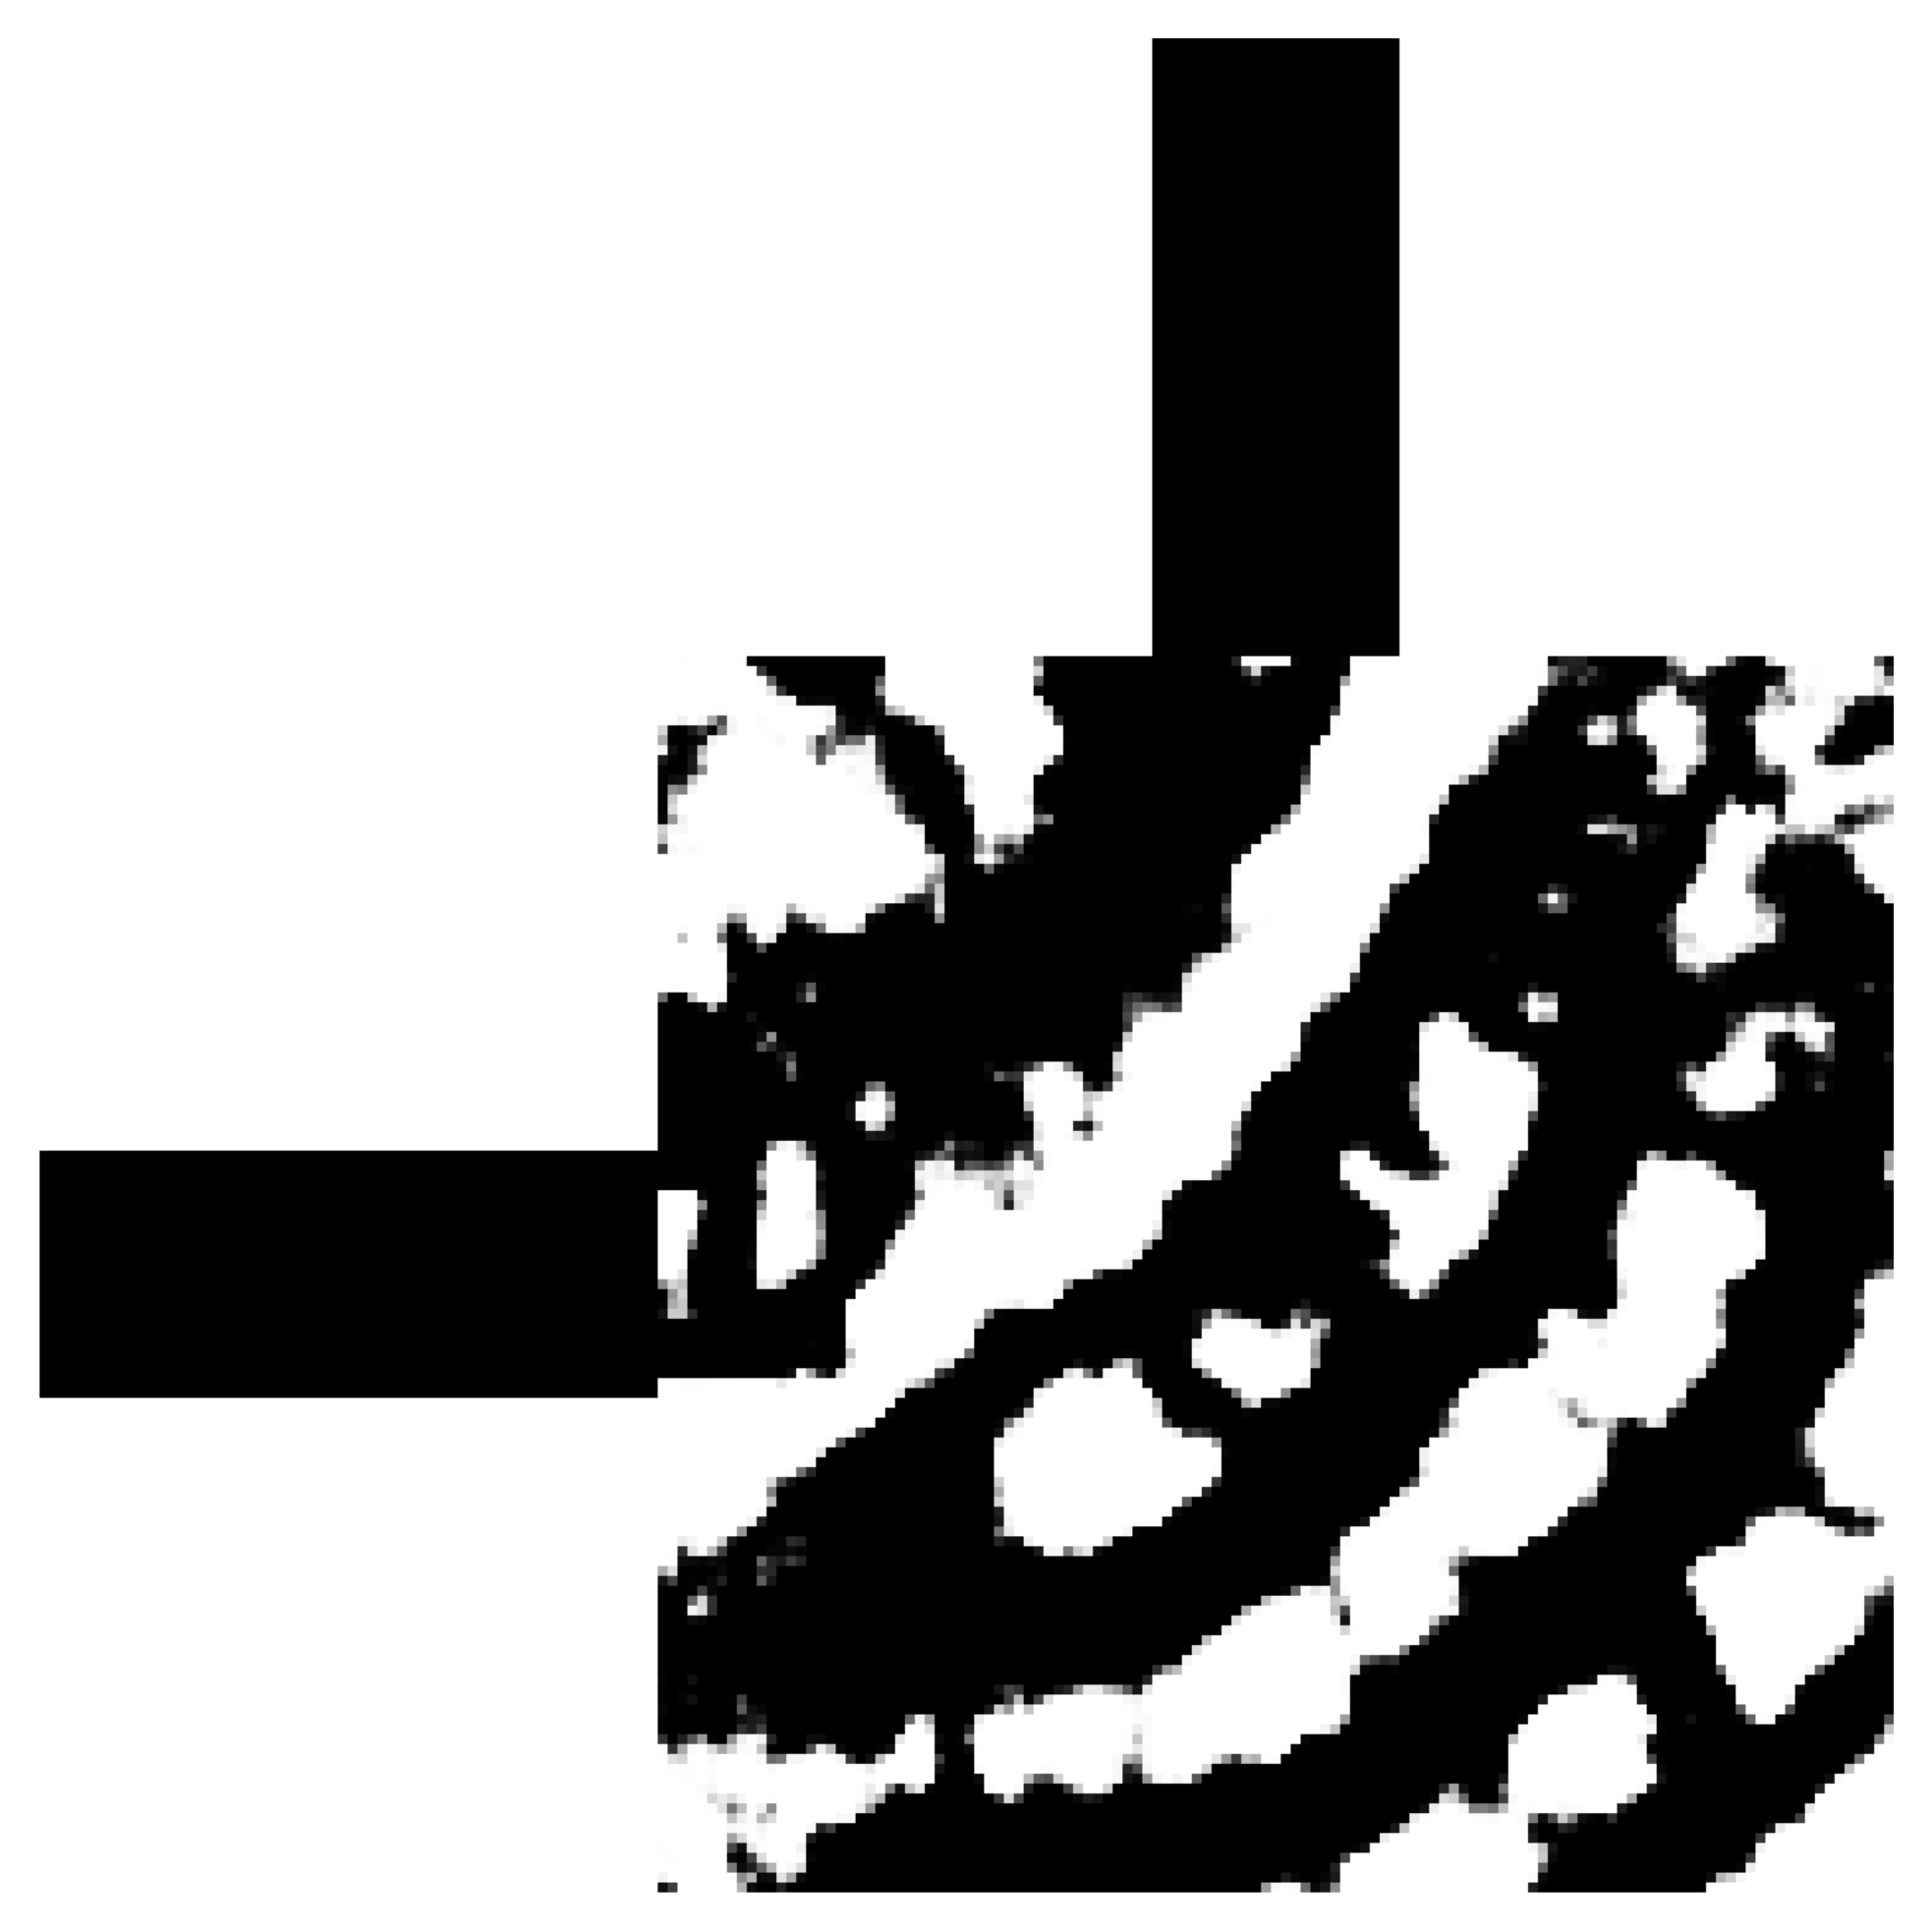
\includegraphics[width=0.4\textwidth]{image/theory/P.png}\label{subfig:P}}
  \hfill
  % filter P
  \subfigure[$\widetilde{\boldsymbol{P}}$ con $r_f = 80 nm$.]
  {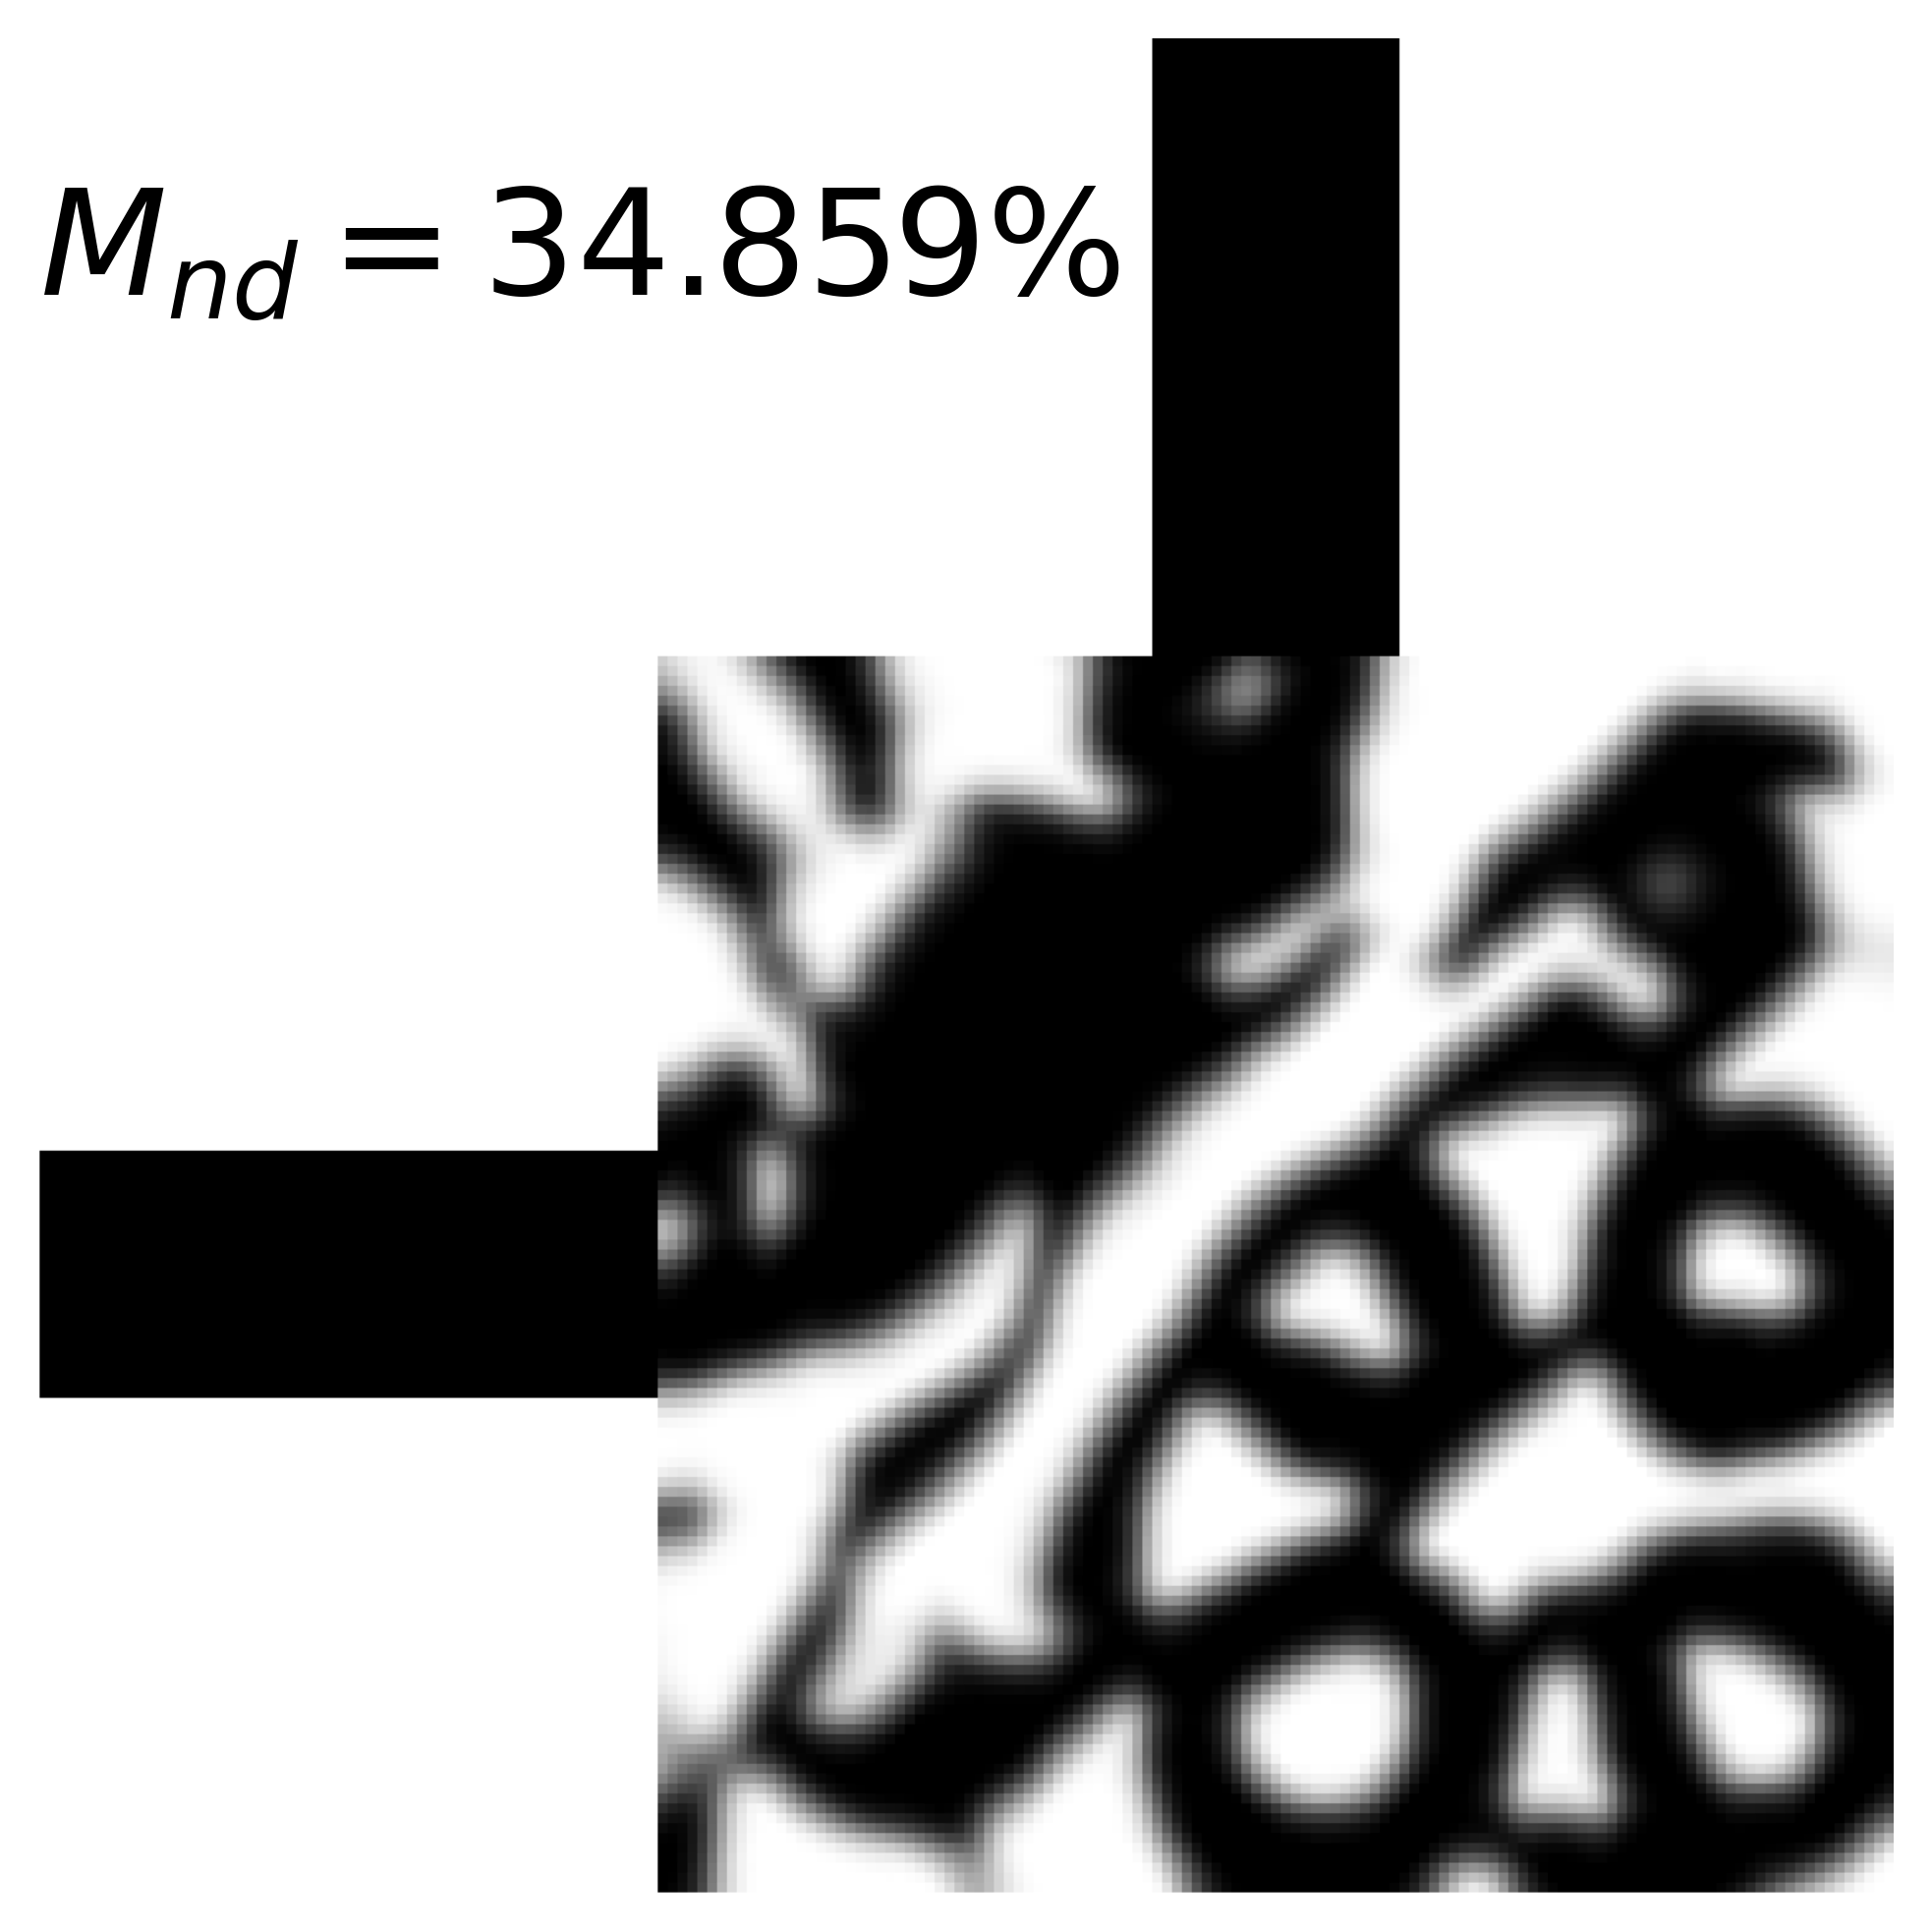
\includegraphics[width=0.4\textwidth]{image/theory/P_filter.png}\label{subfig:P_filter}}

  % 2° row
  \subfigure[$\widetilde{\widetilde{\boldsymbol{P}}}$ con $\eta_d = 0.3$ y $\beta = 2^6$.]
  {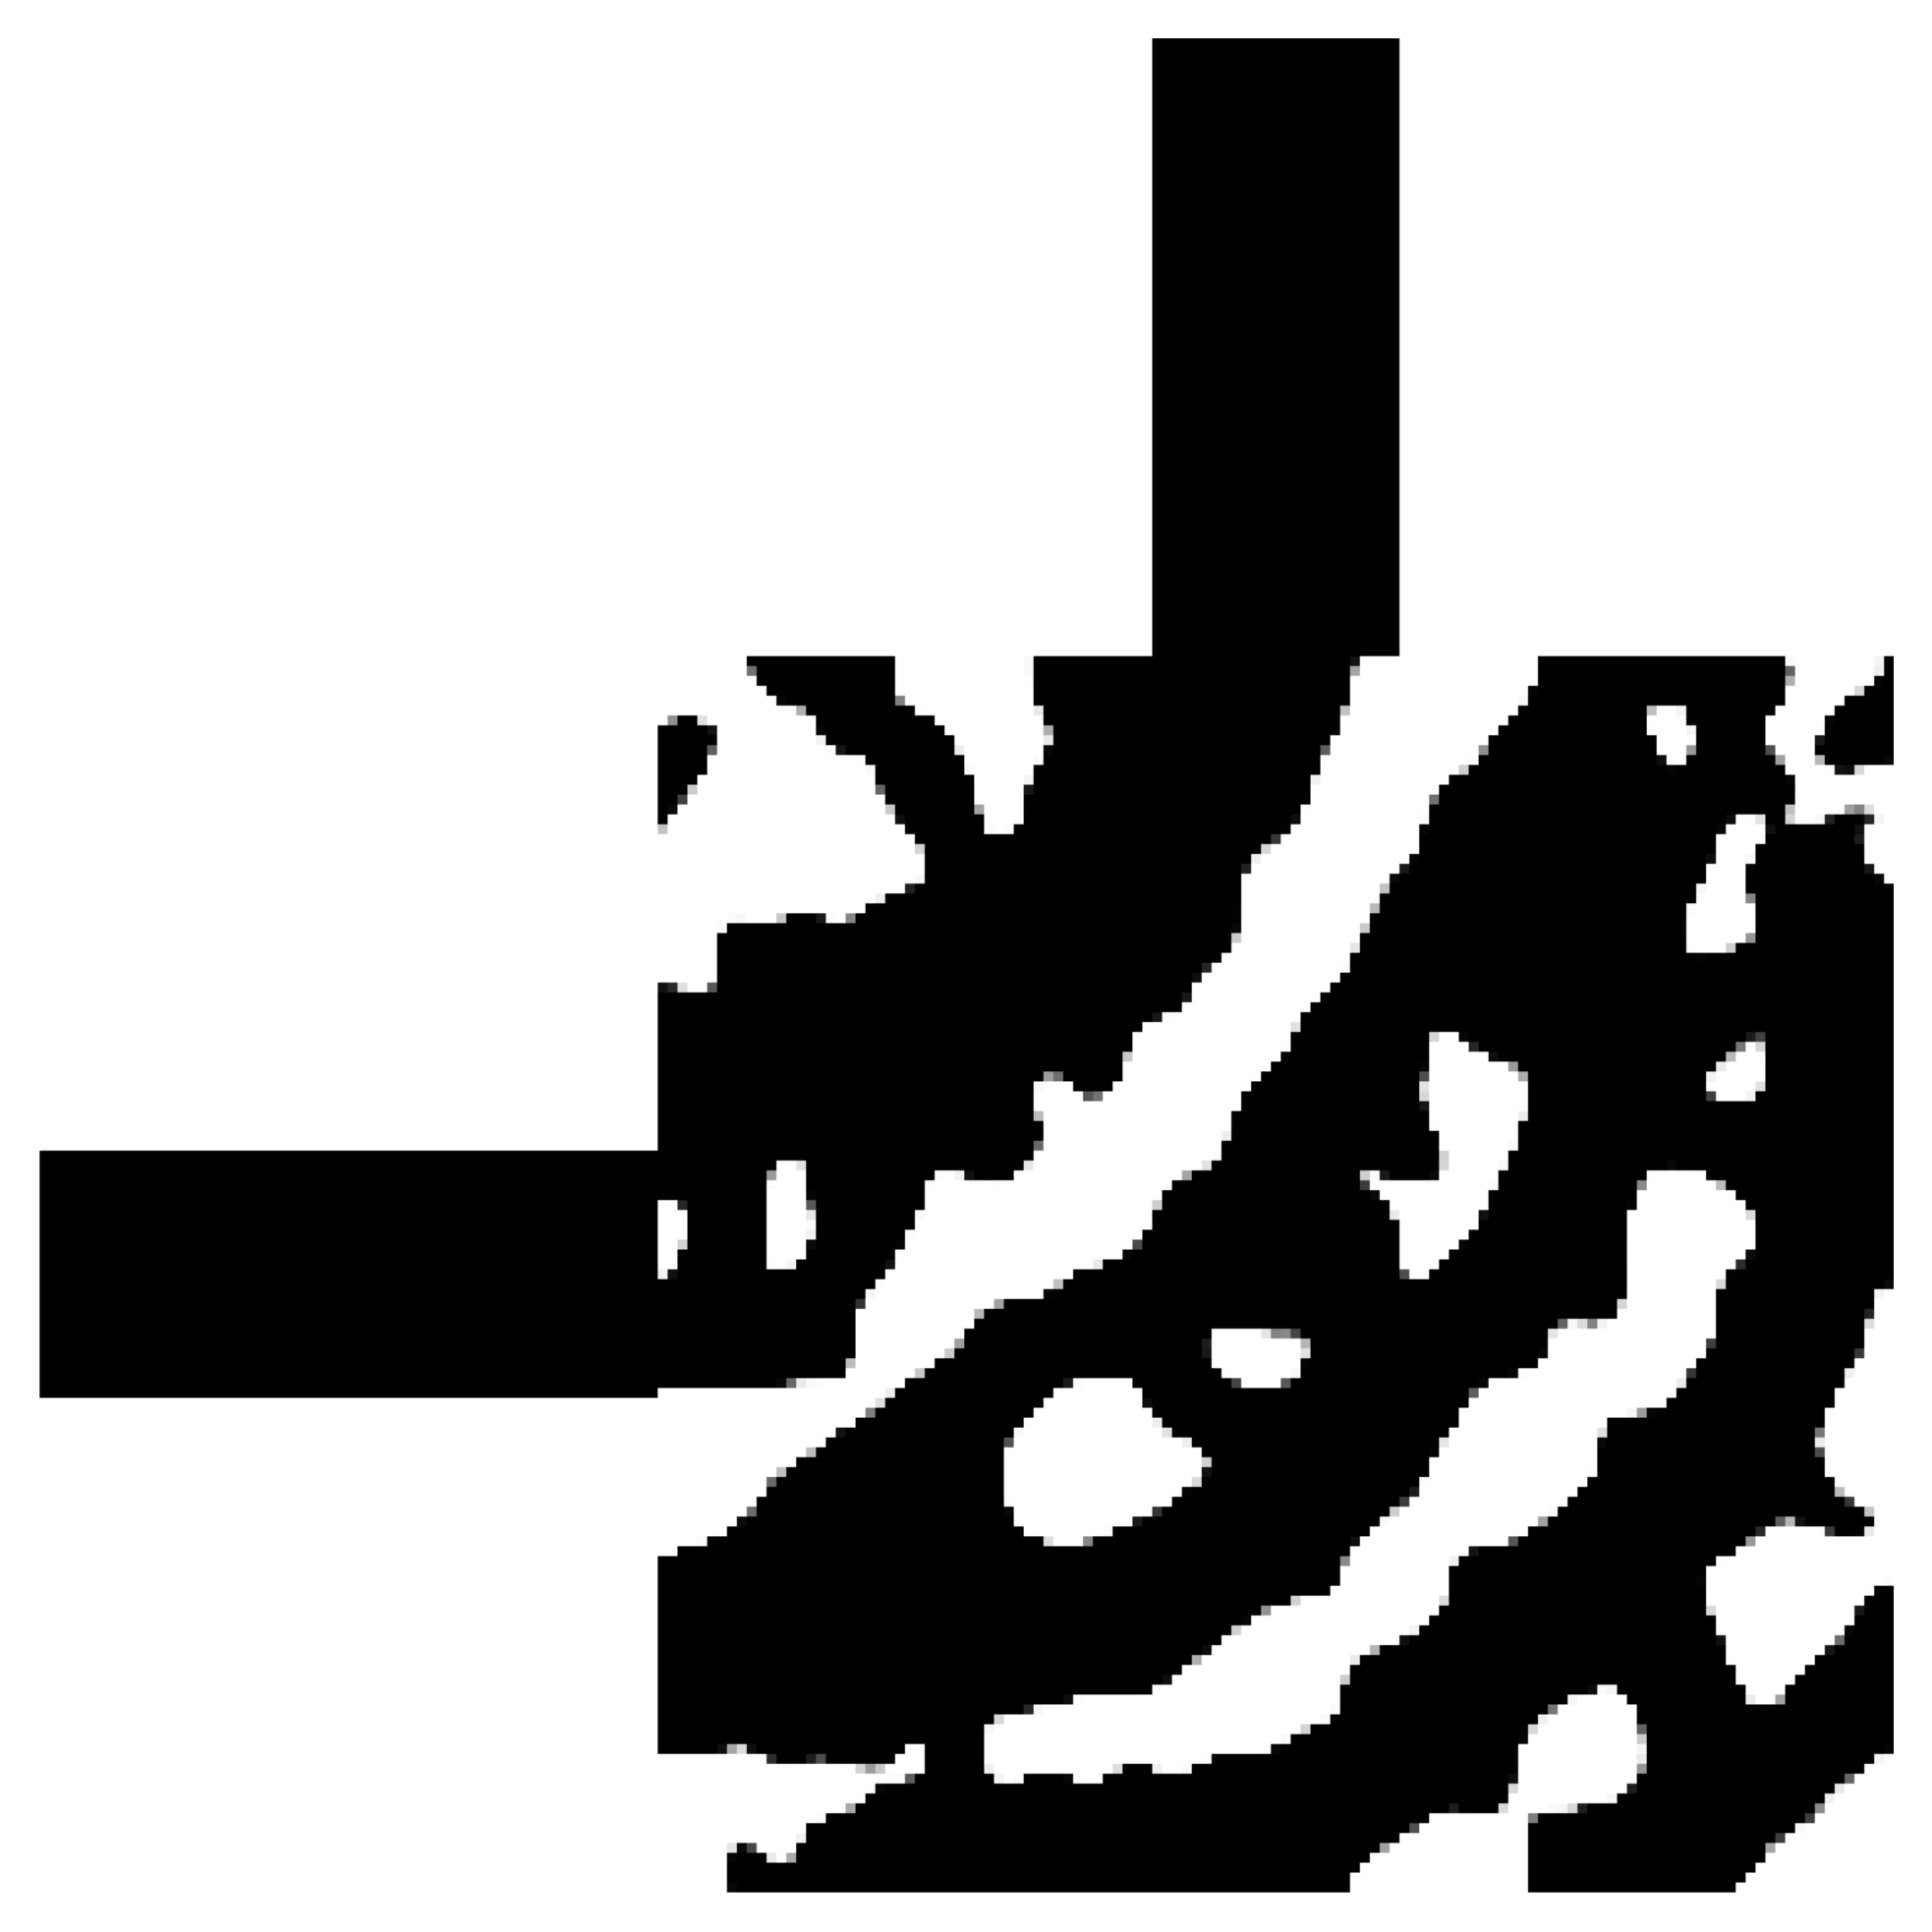
\includegraphics[width=0.3\textwidth]{image/theory/P_E_D.png}\label{subfig:P_E_D}}
  \hfill
  \subfigure[$\widetilde{\widetilde{\boldsymbol{P}}}$ con $\eta_i = 0.5$ y $\beta = 2^6$.]
  {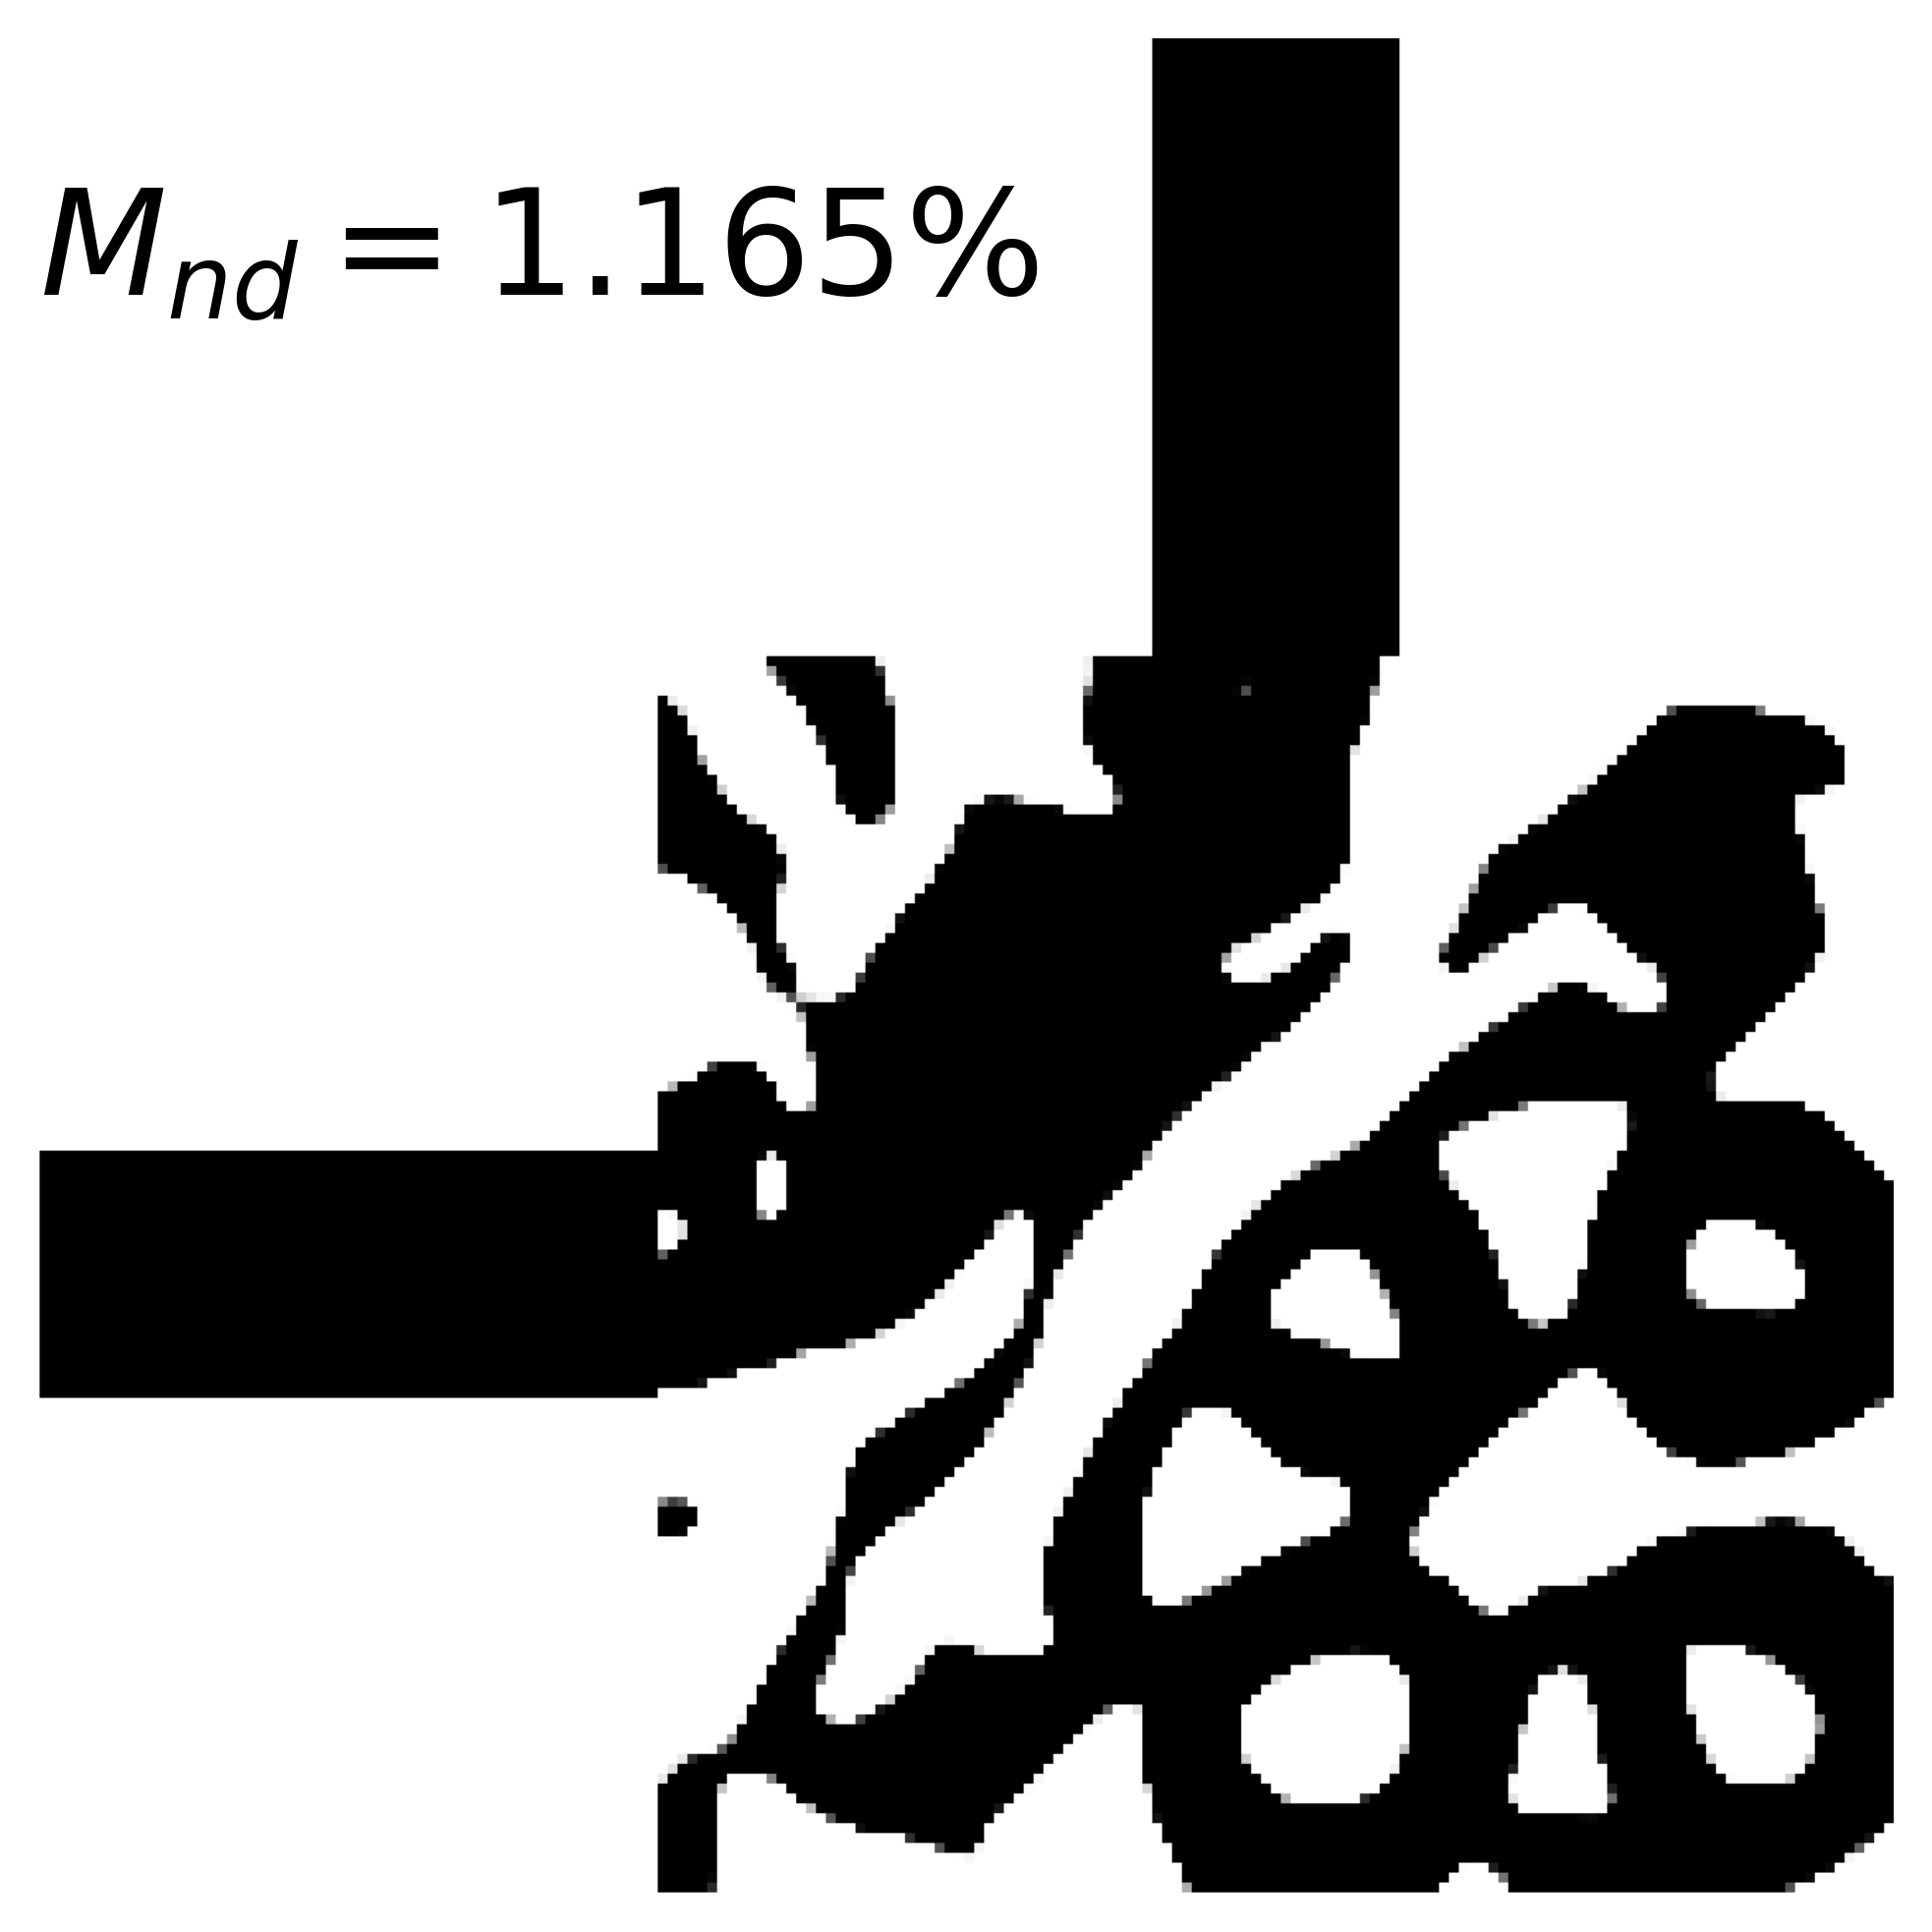
\includegraphics[width=0.3\textwidth]{image/theory/P_E_I.png}\label{subfig:P_E_I}}
  \hfill
  \subfigure[$\widetilde{\widetilde{\boldsymbol{P}}}$ con $\eta_e = 0.7$ y $\beta = 2^6$.]
  {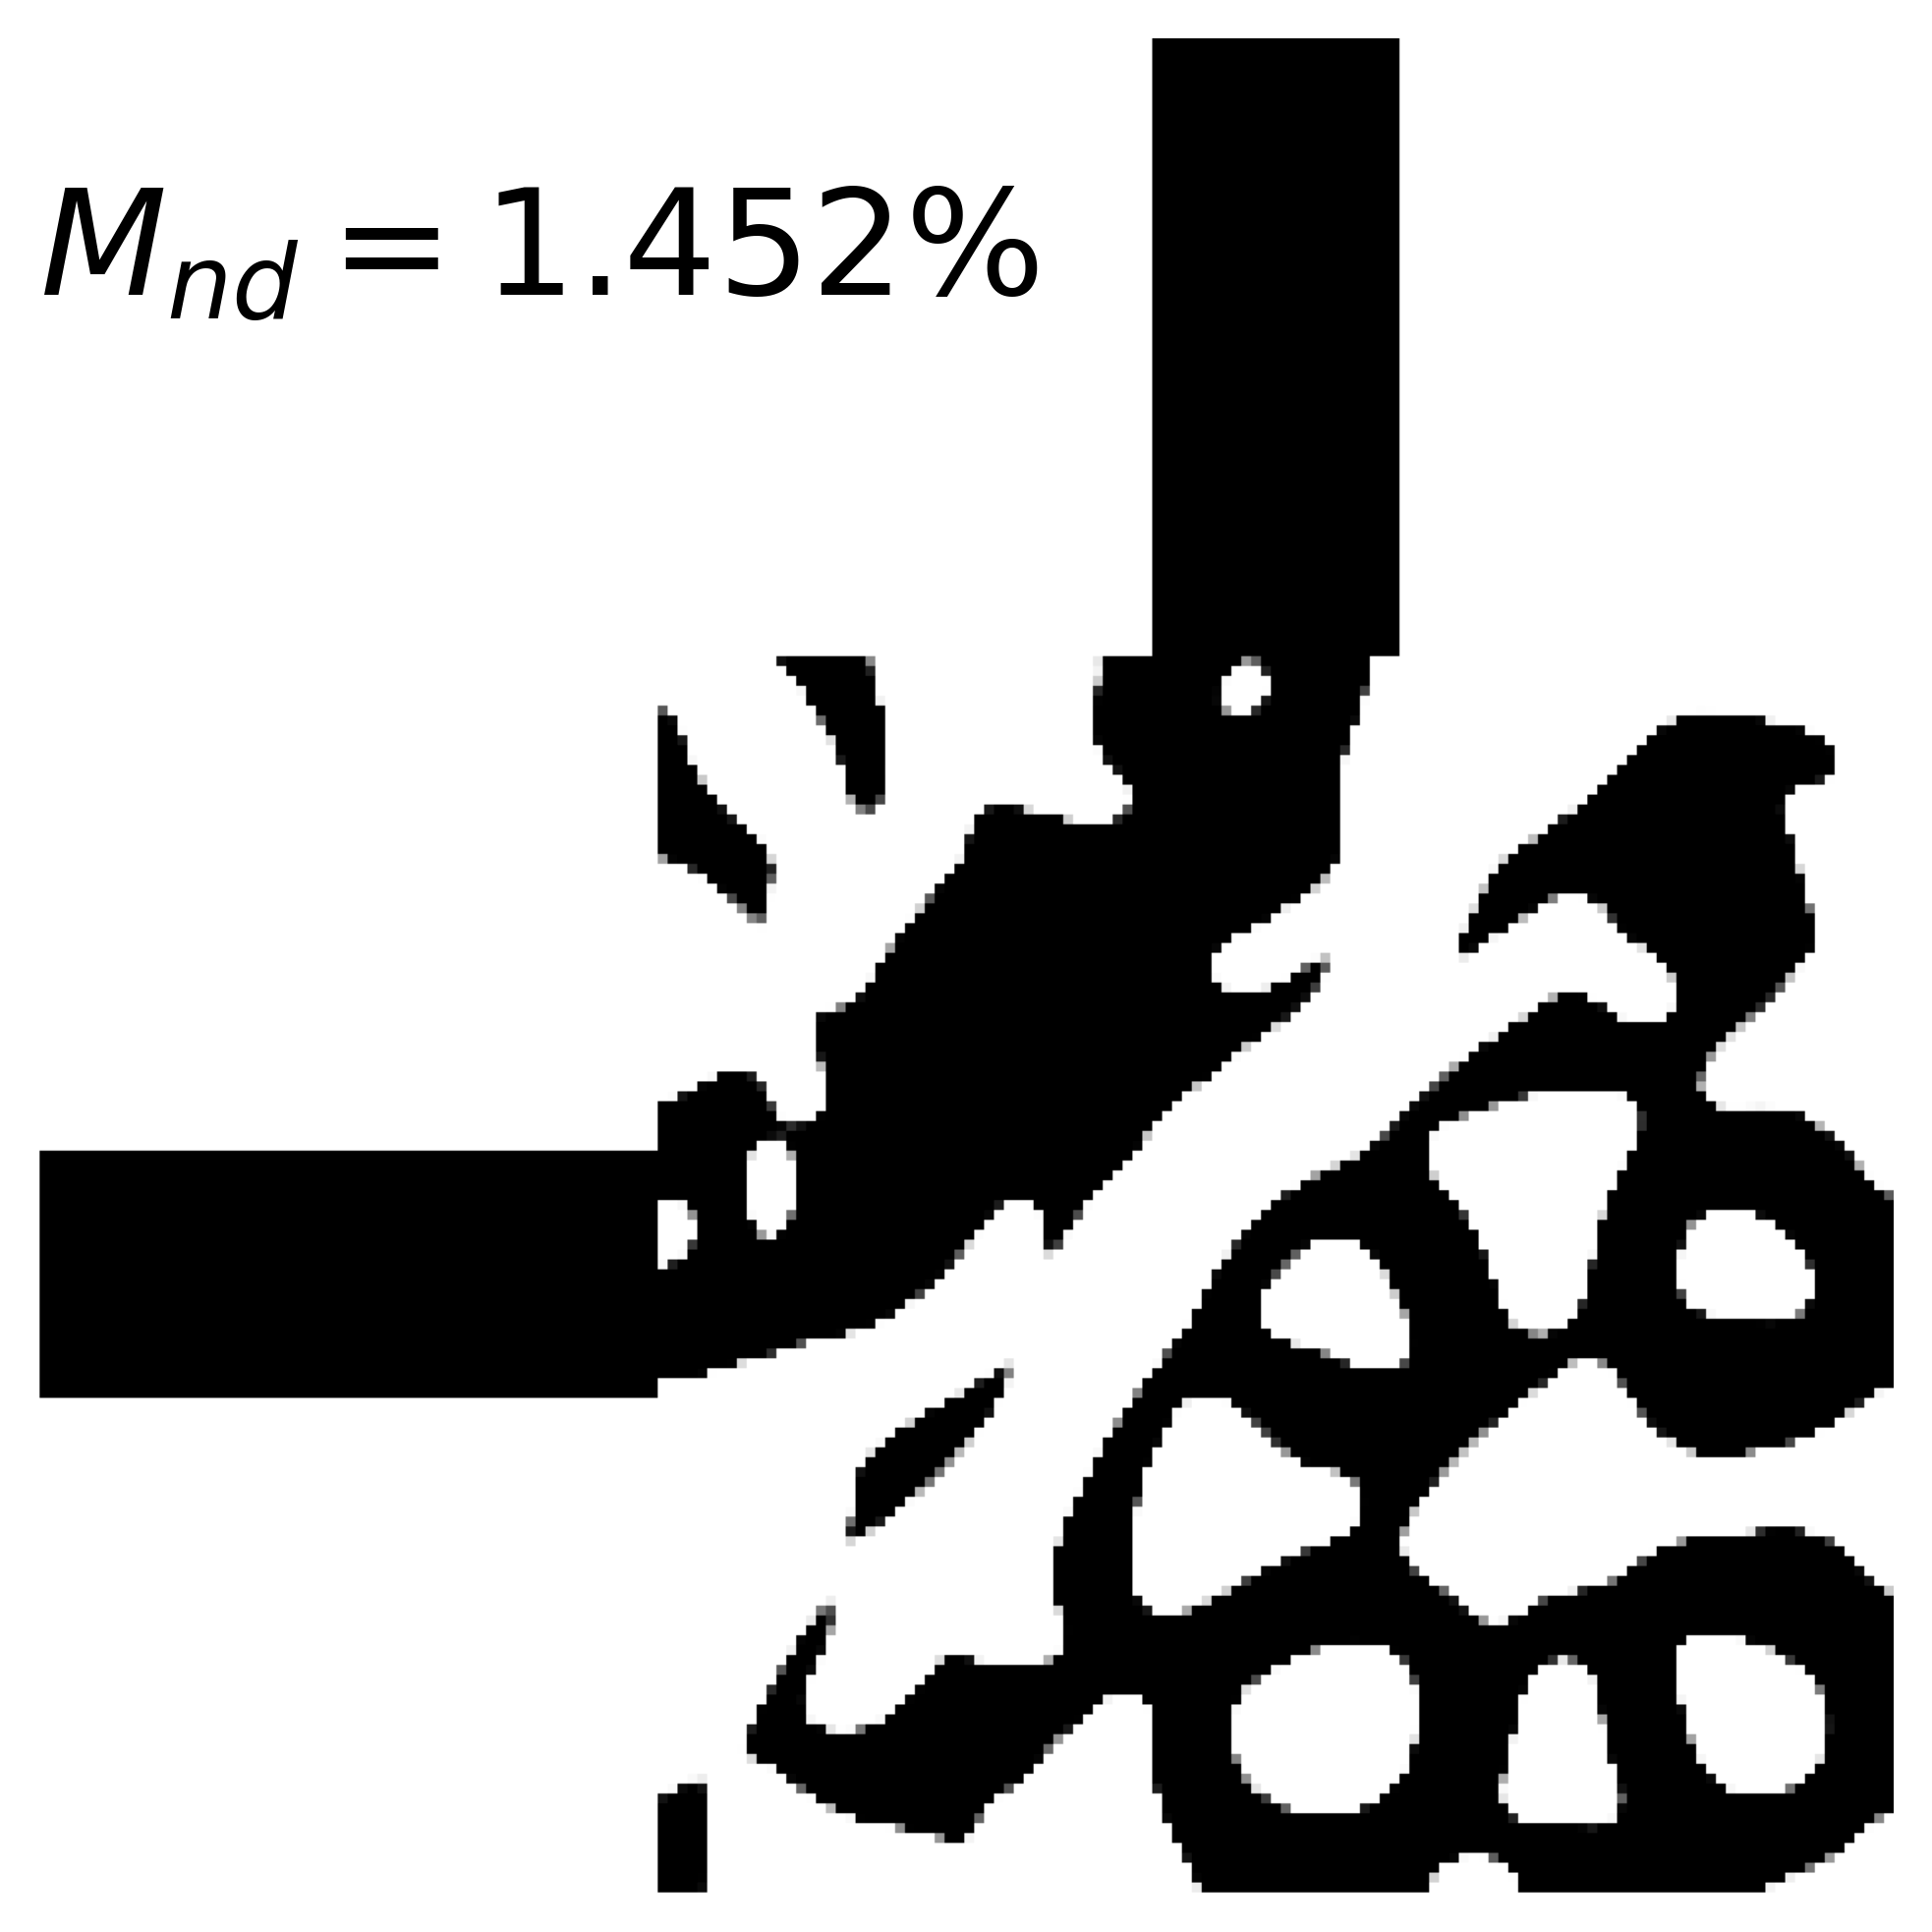
\includegraphics[width=0.3\textwidth]{image/theory/P_E_E.png}\label{subfig:P_E_E}}

  \caption{Aplicación del filtro de densidad y proyección a una parametrización $\boldsymbol{P}.$}
  \label{fig:three-filters}
\end{figure}

Con el objetivo de visualizar estas transformaciones, observemos la \autoref{fig:three-filters}.
En la Figura \autoref{subfig:P} se muestra el diseño que representa una parametrización $\boldsymbol{P}$.
A su derecha se encuentra la Figura \autoref{subfig:P_filter}, aquí aplicamos el filtro de densidad
utilizando un radio de curvatura $r_f = 80 nm$. Como podemos observar, este diseño posee regiones grises,
mas ha logrado eliminar zonas puntiagudas.
Seguidamente, en las Figuras \autoref{subfig:P_E_D}, \autoref{subfig:P_E_I}, \autoref{subfig:P_E_E}
se muestra el diseño de la Figura \autoref{subfig:P_filter} tras aplicar la proyección descrita con
$\beta = 2^6$ y distintos valores de $\eta$.
Al utilizar $\eta = \eta_i = 0.5$ (Figura \autoref{subfig:P_E_I}) 
estamos discretizando el diseño.
Por otro lado, al usar $\eta = \eta_d = 0.3$ (Figura \autoref{subfig:P_E_D})
simulamos que el diseño se ha dilatado 
(i.e., la región de $Si$ del diseño intenta expandirse).
Finalmente, al usar $\eta = \eta_e = 0.7$ (Figura \autoref{subfig:P_E_E})
simulamos que el diseño ha erosionado 
(i.e., la región de $SiO_2$ del diseño intenta expandirse).


Así, observamos como la proyección presentada en esta sección no solo nos permite discretizar diseños,
sino también simular una dilatación o erosión de estos.
Particularmente, la optimización topológica se considera robusta cuando
tiene en cuenta estas dos posibles modificaciones en el proceso de optimización.
Por otro lado, del mismo modo que se aplicó en la \autoref{fig:three-filters}, para poder diferenciar 
el uso de $\eta$ denotaremos como $\eta_i$ al valor usado en un diseño nominal, 
$\eta_e$ para los diseños erosionados y $\eta_d$ para los diseños dilatados.
Además, es importante señalar que se suele escoger los valores de $\eta_e$ y $\eta_d$
de las manera que $\eta_d = 1 - \eta_e$.
Por último, notemos que estos parámetros deben seleccionarse con cuidado; 
caso contrario, el diseño podría representar una dilatación o erosión muy exageradas  \citep{Lazarov2016}.

Un último punto a considerar es que nuestro proceso de optimización necesitará calcular 
$\nabla f_{obj}(\boldsymbol{P})$, pero al aplicar estas transformaciones terminaremos calculando
$\nabla f_{obj}(\widetilde{\widetilde{\boldsymbol{P}}})$.
Para solucionar este problema podemos implementar las transformaciones presentadas 
de manera que aprovechen la diferenciación automática (similar a lo realizado en la implementación
de MEEP \citep{Oskooi2010}); sin embargo, en el presente trabajo optamos por un enfoque más sencillo
que consiste en utilizar la \autoref{eq:densityfiltergrad} y la \autoref{eq:projection-grad} 
para realizar el cálculo utilizando lo siguiente:

\begin{equation}
  \frac{\partial f_{obj}}{\partial \boldsymbol{P}(x, y)} = \displaystyle\sum_{(x', y') \in \overline{B}_{r_f}(x, y)}
  \frac{\partial f_{obj}}{\partial \widetilde{\widetilde{\boldsymbol{P}}}(x', y')}
  \frac{\partial \widetilde{\widetilde{\boldsymbol{P}}}(x', y')}{\partial \widetilde{\boldsymbol{P}}(x', y')}
   \frac{\partial \widetilde{\boldsymbol{P}}(x', y')}{\partial \boldsymbol{P}(x, y)}.
  \label{eq:fobjgrad}
\end{equation}

Para finalizar esta sección, se presenta una función para medir la presencia de regiones grises.
Esta función ($M_{nd}$) nos ayudará en la evaluación de los diseños optimizados obtenidos en esta tesis,
si obtenemos un valor menor al 2 \% podremos decir que nuestro diseño ha sido adecuadamente binarizado.

\begin{equation}
  M_{nd} (\boldsymbol{P}) = \frac{\sum_{1 \leq x \leq n \land 1 \leq y \leq m}
  4 \boldsymbol{P}(x, y)(1 - \boldsymbol{P}(x, y))}{n \times m} \times 100 \%.
\label{eq:grayscale}
\end{equation}

Con todo lo descrito en este capítulo, ya tenemos las herramientas necesarias
para plantear la optimización de nuestros dispositivos.

\section{Algoritmos de Optimización}\label{sec:alg-opt}

Notemos que nuestro problema se termina reduciendo a maximizar $f_{obj}$.
Sin pérdida de generalidad, en la presente sección se describen algoritmos
para minimizar la función $f = -f_{obj}$.
Esto es posible ya que maximizar una función es equivalente a minimizar su negativo \citep{Mykel2019}.


Para minimizar la función $f$, sea $\pmb{\mathscr{P}}$ el conjunto de todas las matrices 
$\boldsymbol{P}: [1, n] \times [1, m] \to [0, 1]$, queremos encontrar algún mínimo global 
$\boldsymbol{P^{*}} \in \pmb{\mathscr{P}}$, 
donde este elemento se define como una matriz que satisface que
$f(\boldsymbol{P^{*}}) \leq f(\boldsymbol{P}), \quad \forall \boldsymbol{P} \in \pmb{\mathscr{P}}$. 
Dicho de otra manera, nuestro problema es encontrar $\boldsymbol{P^{*}}$; sin embargo,
esto es una tarea computacionalmente difícil de resolver \citep{Angeris2021}.

Un problema más viable es encontrar $\sigma > 0 \land \boldsymbol{P^{+}} \in \pmb{\mathscr{P}}$ 
tal que 
$f(\boldsymbol{P^{+}}) \leq f(\boldsymbol{P}), \quad \forall \boldsymbol{P} \in \pmb{\mathscr{P}}:
|| \boldsymbol{P} - \boldsymbol{P^{+}}|| < \sigma$.
Es decir, es más práctico encontrar $\boldsymbol{P^{+}}$ (conocido como mínimo local)
el cual es un elemento que es un mínimo global si restringimos el espacio de búsqueda a cierta región
alrededor de este elemento.

Debemos resaltar que ninguno de los algoritmos de esta sección puede asegurar encontrar el mínimo global;
sin embargo, sus estrategias de búsqueda suelen permitir encontrar 
óptimos locales adecuados \citep{Angeris2021, Schneider2019}.
Además, todos estos algoritmos se aseguran de mantener los valores de $\boldsymbol{P}$ en el
intervalo $[0, 1]$ aplicando $\boldsymbol{P}(x, y) \gets max(0, min(1, \boldsymbol{P}(x, y)))$, mas
este detalle se obvia en las explicaciones por simplicidad en la notación.


\leonidas{
Para visualizar las características de algunos de los algoritmos de esta sección, 
a modo de ejemplo se utiliza la 
\autoref{eq:example} para mostrar que estrategias se aplican para minimizar esta función.
En la \autoref{fig:gxy} podemos observar los conjuntos de nivel de la función $g(x, y)$.
La estrella representa el óptimo global.
}

\begin{figure}[ht]
  \centering
  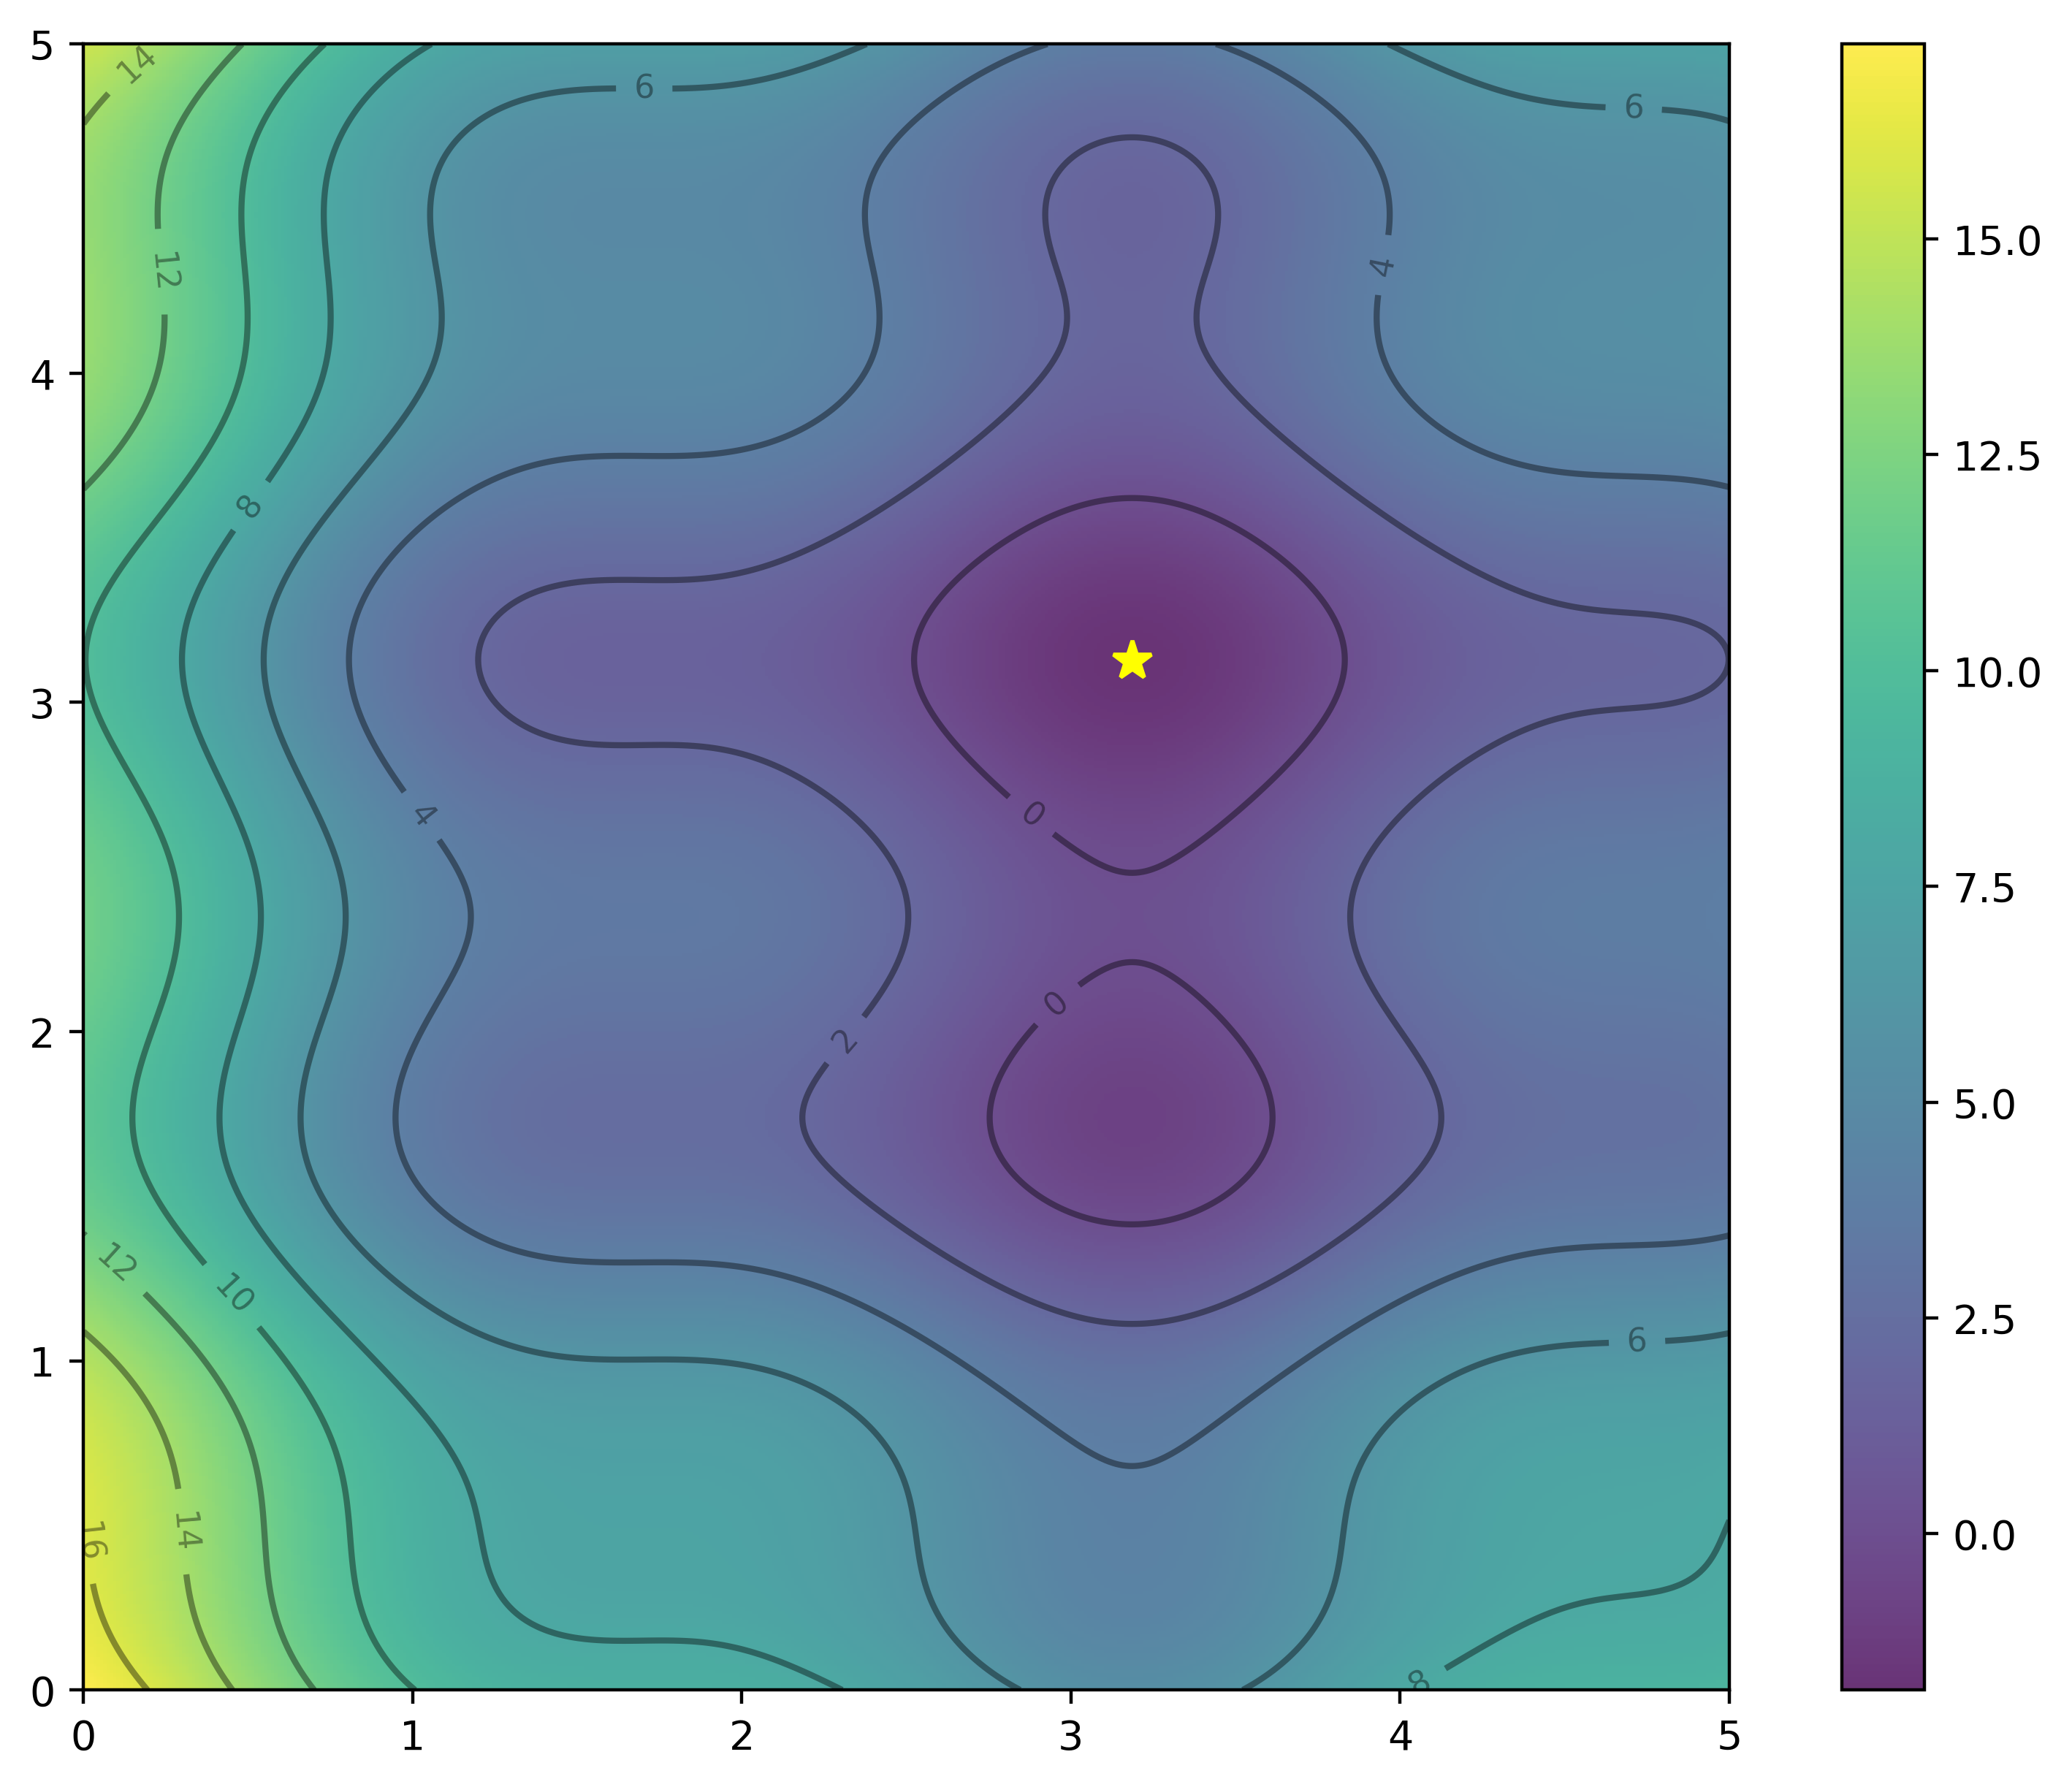
\includegraphics[scale=0.5]{image/theory/countour.png}
   \caption{Contornos de nivel de la función $g(x, y)$.}
  \label{fig:gxy}
\end{figure}


\begin{equation}
  g(x, y) = (x-3.14)^2 + (y-2.72)^2 + sin(3x + 1.41) + sin(4y-1.73).
  \label{eq:example}
\end{equation}

\subsection{\emph{Genetic Algorithms} (GA)}\label{sec:ga}

Como se describe en el Algoritmo \ref{alg:GA} \citep{Mykel2019}, la idea es 
comenzar generando una población (\emph{population}) de tamaño $population\_size$.
Esta población es un conjunto de matrices de $n \times m$ generadas a partir de una parametrización
inicial $\boldsymbol{P}$, línea 1.
Los siguientes tres pasos se ejecutan por $k$ iteraciones.
Primero, se realiza un proceso de selección para obtener las mejores parametrizaciones
(\emph{parents}), línea 3.
Segundo, los seleccionados se encargan de producir la nueva generación
(\emph{children}), línea 4.
Tercero, la nueva generación muta obteniendo nuevas características, línea 5.

\begin{algorithm}
%\footnotesize
\KwData{$\boldsymbol{P}, population\_size, GA\_range, n\_selected\_parents, prob\_mutation$}
\KwResult{$min(population)$}
$population = generate\_population()$ \\
\For{$t = 0; \, t < k; \, t$++}{
    $parents = select(population)$ \\
    $children = crossover(parents)$ \\
    $population = mutation(children)$
}
\caption{\emph{Genetic Algorithms} (GA)}
\label{alg:GA}
\end{algorithm}

Como se observa en el Algoritmo \ref{alg:GA}, tenemos las siguientes funciones:

\begin{itemize}
    \item $generate\_population():$ 
      retorna $population\_size$ matrices 
      $\boldsymbol{P'}$ tal que 
      $|\boldsymbol{P'}(x, y) - \boldsymbol{P}(x, y)| \in U(-GA\_range, GA\_range), \quad \forall x \in [1, n]
      \land y \in [1, m]$.

    \item $select(population):$ 
      retorna $n\_selected\_parents$ elementos de $population$ de
      acuerdo a la probabilidad $prob_i$ dada por la ecuación
    
    \begin{equation}
      prob_i = \frac{max(f) - f^{(i)}}{\displaystyle\sum_{j} max(f) - f^{(j)}},
    \label{eq:prob}
    \end{equation}
    
    donde $f^{(i)}$ representa el valor de $f$ aplicado a la 
    $i-$ésima parametrización de $population$ y $max(f)$ es el máximo
    valor de $f$ al haber sido aplicado a todas las matrices de $population$.
    
    \item $crossover(parents):$ 
    retorna $population\_size$ nuevas parametrizaciones.
    Cada nueva matriz $\boldsymbol{S}$ es la combinación de dos parametrizaciones aleatorias 
    $\boldsymbol{P_1}$ y $\boldsymbol{P_2}$ seleccionados de $parents$.
    En esta combinación, para cada $x \in [1, n] \land y \in [1, m]$ se define 
    con igual probabilidad que
    $\boldsymbol{S}(x, y) = \boldsymbol{P_1}(x, y)$ o
    $\boldsymbol{S}(x, y) = \boldsymbol{P_2}(x, y)$.

    \item $mutation(children):$ 
      retorna $children$, pero
      a cada elemento de todas estas matrices
      le agrega un valor en $U(-GA\_range, GA\_range)$ con
      probabilidad $0 < prob\_mutation < 1$.

\end{itemize}

\leonidas{Para nuestro problema en específico como los valores de la matriz $\boldsymbol{P}$ están en el rango
$[0, 1]$, el parámetro $GA\_range$ también debe encontrarse en este rango. Una selección adecuada
de estos parámetros requiere de experimentación. Los valores usados en este trabajo son detallados
en el \autoref{chapter:methodology}}.

\begin{figure}[ht]
  \centering
  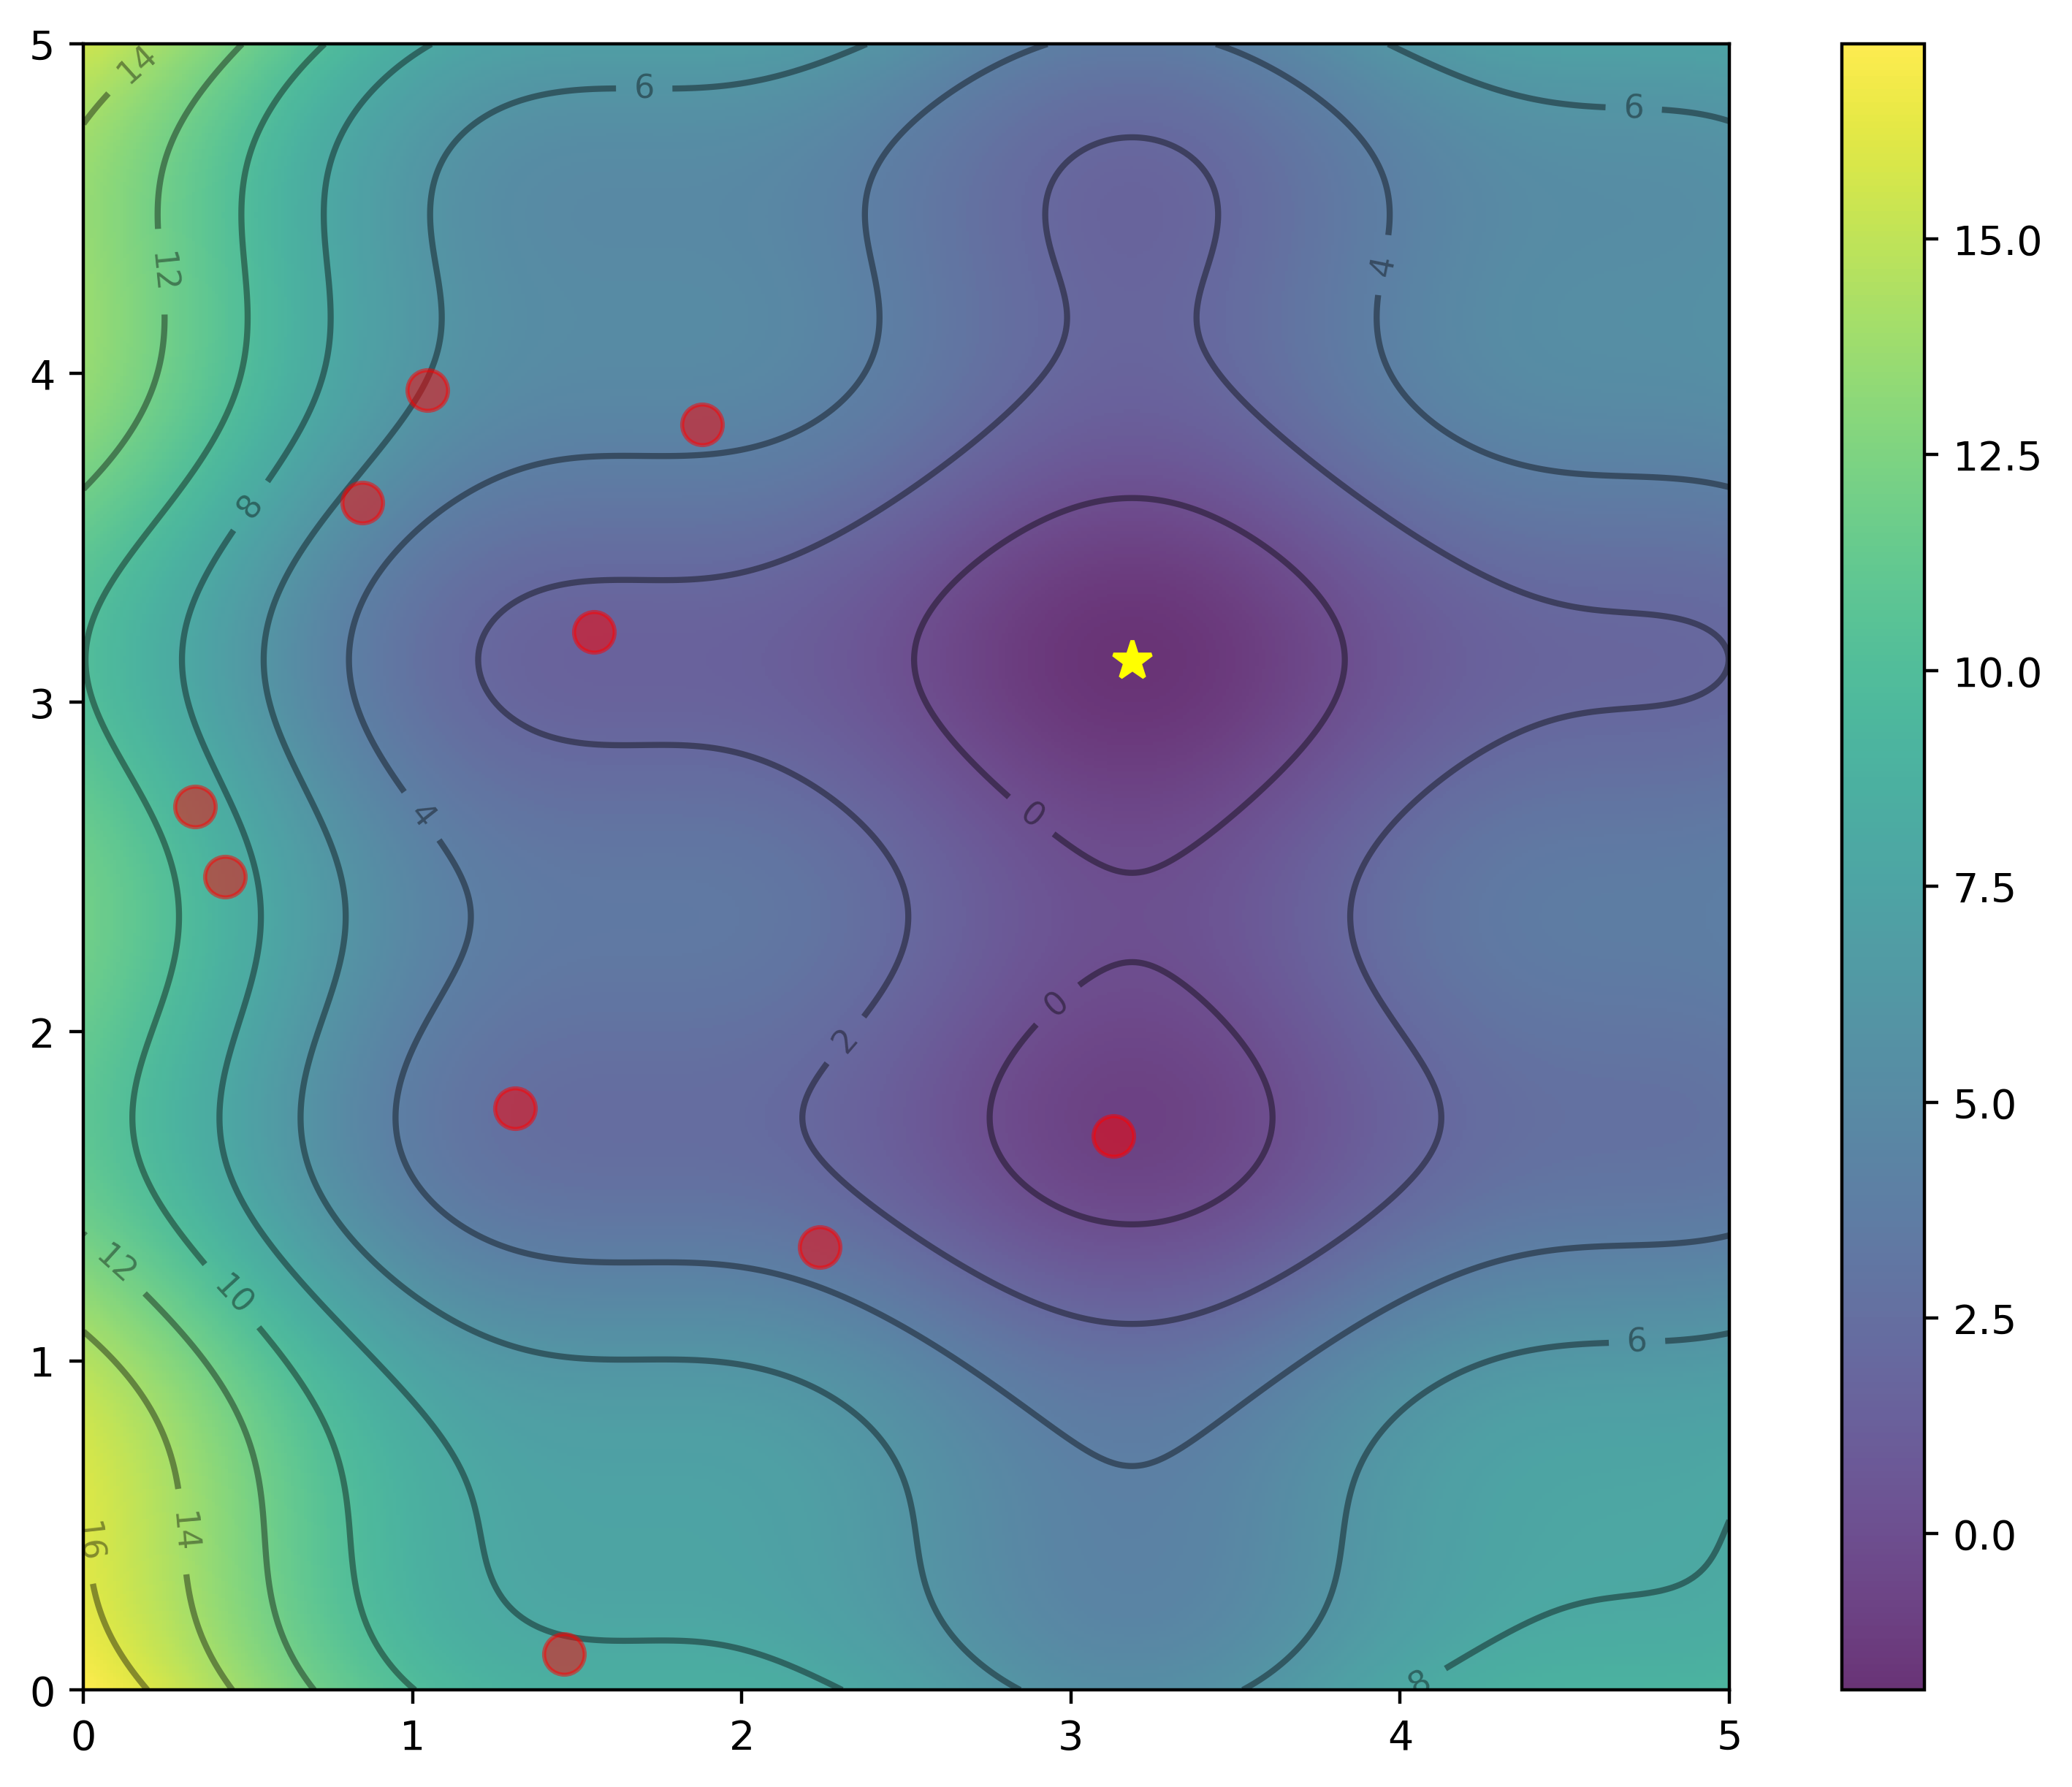
\includegraphics[scale=0.5]{image/theory/GA.png}
   \caption{Visualización del proceso de optimización de $g(x, y)$ usando GA.}
  \label{fig:ga}
\end{figure}

\leonidas{
En la \autoref{fig:ga} se visualiza como GA optimiza $g(x, y)$ comenzando
con distribuir puntos aleatorios en el espacio de búsqueda. Luego, 
de forma iterativa sigue los pasos descritos en el Algoritmo \ref{alg:GA}
para intentar encontrar el óptimo global (i.e., la estrella).
}

\subsection{\emph{Particle Swarm Optimization} (PSO)}\label{sec:pso}

Podemos pensar este algoritmo como un caso especial del Algoritmo \ref{alg:GA}
\citep{Mykel2019}.
La idea es visualizar el $i-$ésimo individuo como una partícula definida por 
su posición ($\boldsymbol{P^{(i)}}$), velocidad ($\boldsymbol{V}^{(i)}$) y 
la mejor posición encontrada por la partícula ($\boldsymbol{P^{(i)}_b}$).
Para nuestro problema la matriz de parametrización representa la posición y
la velocidad es una matriz que guía la exploración a otras parametrizaciones.

La idea principal del algoritmo es que cada partícula acumula 
velocidad en una dirección favorable dada por: 
(i) la mejor posición encontrada hasta el momento por esta partícula y 
(ii) la mejor posición encontrada por la población completa.
Como consecuencia, los individuos se pueden mover independientemente de
perturbaciones locales.
Adicionalmente, agregando caminos aleatorios los individuos incorporan
comportamientos impredecibles que puede permitirles encontrar potenciales
mejores elementos. Esta idea se sintetiza en el Algoritmo \ref{alg:PSO}.

\begin{algorithm}
%\footnotesize
\KwData{$\boldsymbol{P}, population\_size, PSO\_range, \omega, c_1, c_2$}
\KwResult{$\boldsymbol{P_b}$}
$population = generate\_population()$ \\
\For{$t = 0; \, t < k; \, t$++}{
    $\boldsymbol{P_b} = select(population)$ \\
    $population = mutation(population, \boldsymbol{P_b})$
}
\caption{\emph{Particle Swarm Optimization} (PSO)}
\label{alg:PSO}
\end{algorithm}

Como se observa en el Algoritmo \ref{alg:PSO}, tenemos las siguientes funciones:

\begin{itemize}

    \item $generate\_population():$ 
      retorna $population\_size$ matrices 
      $\boldsymbol{P'}$ tal que 
      $|\boldsymbol{P'}(x, y) - \boldsymbol{P}(x, y)| \in U(-PSO\_range, PSO\_range), \quad \forall x \in [1, n]
      \land y \in [1, m]$. Además genera las matrices $V$ con valores en $U(0, 1)$.

\item $select(population):$ retorna el individuo con el menor valor de $f$ encontrado hasta el momento.

\item $mutation(population, \boldsymbol{P_b}):$ Aplica las siguientes transformaciones a \emph{population}: 
    
  \begin{equation}
    \boldsymbol{P^{(i)}} \gets \boldsymbol{P^{(i)}} + \boldsymbol{V^{(i)}},
  \label{pso-pos}
  \end{equation}

  \begin{equation}
    \boldsymbol{V^{(i)}} \gets \omega \boldsymbol{V^{(i)}} + \
                          c_1 r_1 \left(\boldsymbol{P_{b}^{(i)}} - \boldsymbol{P^{(i)}} \right) + \
                          c_2 r_2 \left(\boldsymbol{P_{b}} - \boldsymbol{P^{(i)}} \right),
  \label{pso-speed}
  \end{equation}
    

  donde $\boldsymbol{P_{b}}$  es la mejor posición encontrada globalmente, 
  $\omega$ representa la tendencia de la partícula de conservar su velocidad actual,
  $c_1$ y $c_2$ cuantifica la atracción relativa con $\boldsymbol{P_{b}^{(i)}}$ y 
  $\boldsymbol{P_{b}}$ respectivamente, 
  y $r_1, r_2 \in U(0, 1)$ representan el comportamiento impredecible.


\end{itemize}

\leonidas{Para nuestro problema en específico $PSO\_range \in [0, 1]$ y su selección require de experimentación. 
Por otro lado, es válido experimentar usando 
$\omega = c_1 = c_2 = 0.5$ basándonos en el trabajo de \cite{Schneider2019}}.


\begin{figure}[ht]
  \centering
  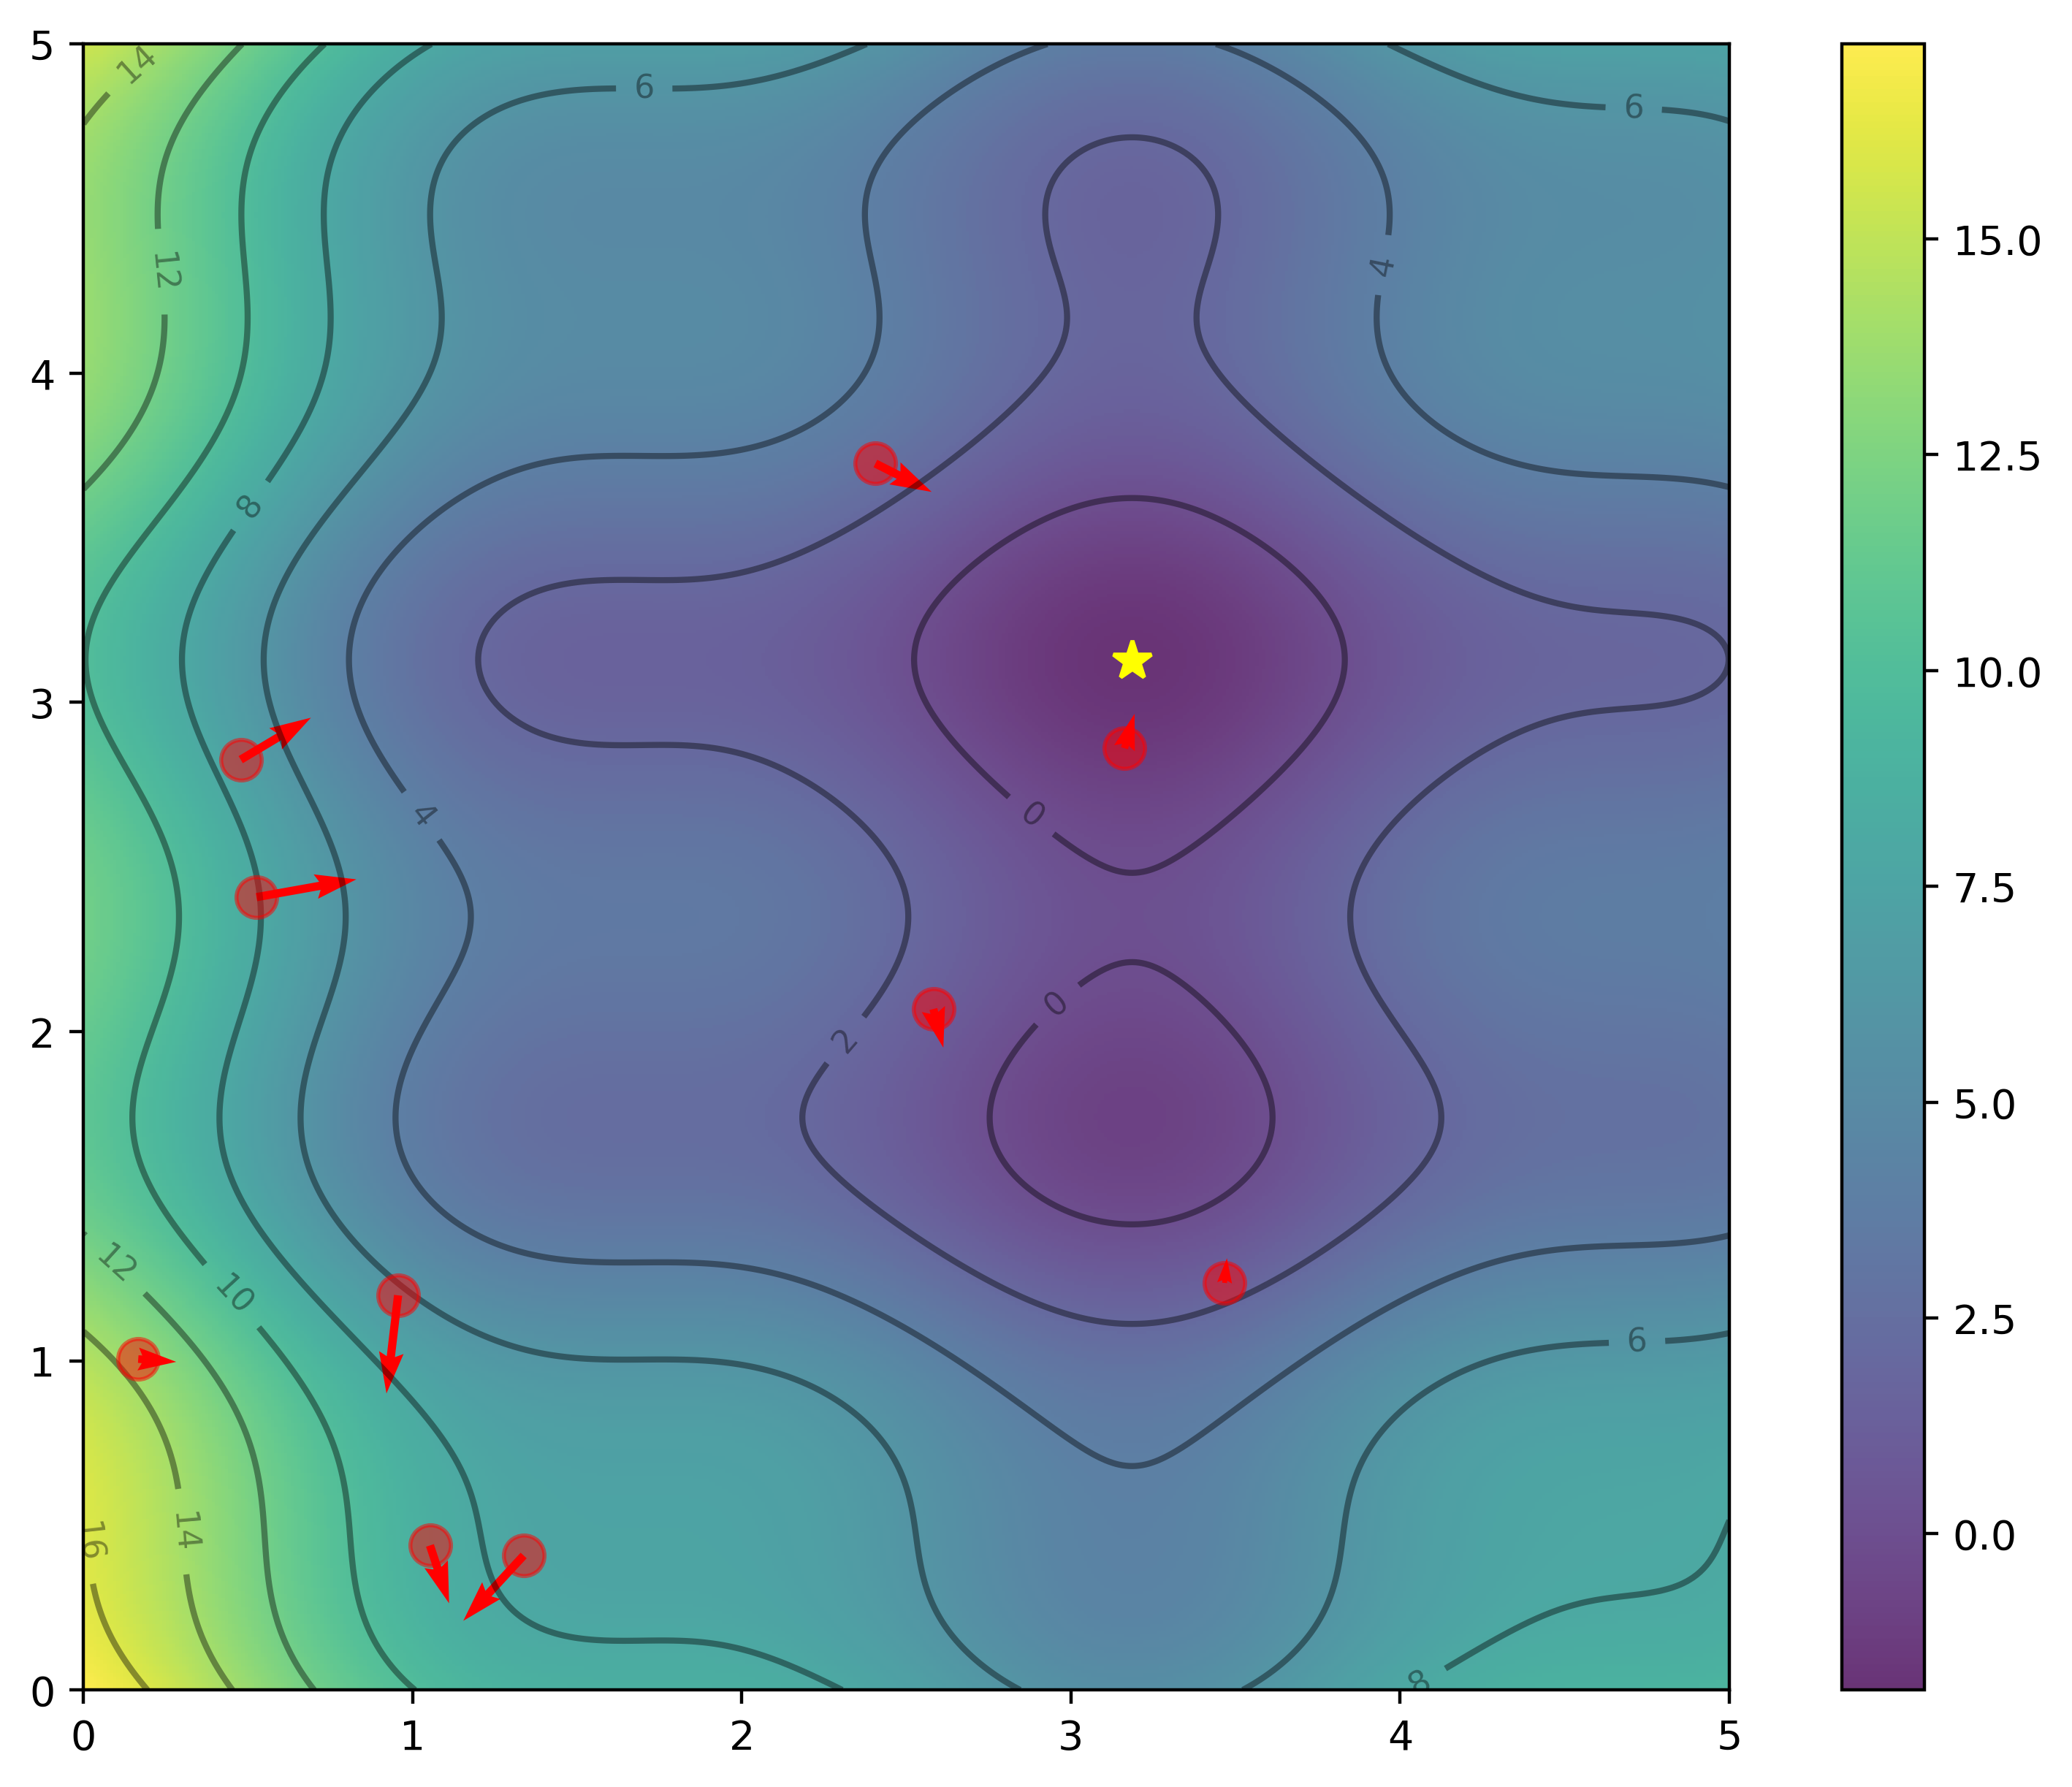
\includegraphics[scale=0.5]{image/theory/PSO.png}
   \caption{Visualización del proceso de optimización de $g(x, y)$ usando PSO.}
  \label{fig:pso}
\end{figure}

\leonidas{
En la \autoref{fig:pso} se visualiza como PSO optimiza $g(x, y)$ comenzando
con distribuir puntos aleatorios en el espacio de búsqueda. 
Adicionalmente, se observa que cada punto tiene asociado una flecha de tamaño y dirección variable.
Esto es para representar que cada partícula intentará explorar, potencialmente, en distintas regiones
del espacio de búsqueda y avanzando distintas distancias.
En siguientes iteraciones las partículas se irán dirigiendo hacia la partícula que globalmente ha encontrado
el mejor resultado. La velocidad de este proceso depende de la elección de los parámetros.
}


\subsection{\emph{Covariance Matrix Adapatation Evolution Strategy} (CMA-ES)}\label{sec:cma-es}

La idea general de esta estrategia evolutiva, mostrada en el Algoritmo
\ref{alg:CMA}, es mantener:
(i) un vector $\boldsymbol{\mu}$ $p$-dimensional,
(ii) una matriz $\boldsymbol{C}$ y
(iii) un número $\sigma$ para ir generando $n$ individuos $p$-dimensionales
a partir una distribución $\mathcal{N}(\mu,\,\sigma^{2} \boldsymbol{C})$.


Tomar puntos de esta distribución limita el espacio de búsqueda a una
hiperelipse.
Así, el algoritmo evalúa puntos en esta región limitada.
Luego, usando los valores obtenidos, se puede decidir entre:
(i) mover la hiperelipse a otra región del espacio de búsqueda
(ii) expandir o reducir la región cubierta por la distribución.
El algoritmo de CMA-ES trabaja iterativamente sobre esta idea hasta que la
hiperelipse termina casi degenerándose en un punto, 
potencialmente un óptimo.

\begin{algorithm}
  \KwData{$\boldsymbol{P}, population\_size, \sigma$}
\KwResult{$\boldsymbol{\mu}$}
$\boldsymbol{\mu} = flatten(\boldsymbol{P})$ \\
\For{$t = 0; \, t < k; \, t$++}{
  sample() \tcp{Obtener $population\_size$ puntos de $\mathcal{N}(\boldsymbol{\mu},\,\sigma^{2} \boldsymbol{C})$}
    update() \tcp{Ecuación \ref{cma-average}}
    control() \tcp{Ecuación \ref{cma-control}}
    adapt() \tcp{Ecuación \ref{cma-adapt}}
}
\caption{CMA-ES}
\label{alg:CMA}
\end{algorithm}


Entrando en más detalles del Algoritmo \ref{alg:CMA},
en la línea 1 simplemente se linealiza la matriz $\boldsymbol{P}$ en un vector $\boldsymbol{\mu}$ 
de dimensión $p = n \times m$ (i.e., se unen sus vectores filas de manera consecutiva para formar un solo vector).
Luego, dentro del bucle en la iteración $t$, en la línea 3 se genera $population\_size$ puntos
$p$-dimensionales $\boldsymbol{x_i}$ de la distribución $\mathcal{N}(\boldsymbol{\mu},\,\sigma^{2} \boldsymbol{C})$, 
donde estos son ordenados ascendentemente de acuerdo
al valor de $f$.
En la línea 4 actualizamos la media $\boldsymbol{\mu}$ usando el promedio ponderado dado
por

\begin{equation}
  \boldsymbol{\mu^{(t + 1)}} \gets \sum_{i=1}^{n} w_i \boldsymbol{x_i},
\label{cma-average}
\end{equation}

donde $w_i$ son valores fijos y escogidos de tal manera que proporcionen mayor
contribución a los puntos con menor valor al evaluarlos en $f$. 
Esto permite mover la media $\boldsymbol{\mu}$ en una dirección favorable.

Seguidamente, se necesita actualizar $\sigma$ para expandir o reducir la
hiperelipse en la siguiente iteración. Por este motivo, la línea 5 controla
este valor mediante las ecuaciones

\begin{equation}
    \sigma^{(t + 1)} \gets \sigma^{(t)} \exp\bigg(\frac{c_{\sigma}}{d_{\sigma}}
    \underbrace{\left(\frac{||\boldsymbol{p_{\sigma}}||}{\mathbb{E}||\mathcal{N}(0,
    \mathbf{I})||} - 1 \right)}_{\text{evolution path comparison}} \bigg),
\label{cma-control}
\end{equation}

\begin{equation}
\mathbb{E}||\mathcal{N}(0, \mathbf{I})|| = \sqrt{2} \left(
  \frac{\Gamma\left(\frac{p + 1}{2}\right)}{\Gamma\left({\frac{p}{2}}\right)}
  \right),
\label{cma-E}
\end{equation}

donde $\boldsymbol{p_{\sigma}}$ es una variable que acumula los pasos llevados,
$c_{\sigma} \in [0, 1]$ es una variable que determina el tiempo acumulado para $p_{\sigma}$ y 
$d_{\sigma} \approx 1$ es un parámetro que determina el ratio de posibilidad de cambio de $\sigma^{(t + 1)}$. 
La principal parte de la \autoref{cma-control} es el término \emph{evolution path comparison}, 
aquí se compara el tamaño de $p_{\sigma}$ con su tamaño esperado bajo selección
aleatoria.
De esta comparación podemos controlar si el valor de $\sigma$ debe
incrementarse, disminuirse o permanecer igual.

Finalmente, en la línea 6 cambiamos $\boldsymbol{C}$ a una dirección favorable usando lo siguiente:

\begin{multline}
  \boldsymbol{C^{(t + 1)}} \gets \overbrace{\bigg(1 - c_1 c_c (1 - h_{\sigma})(2 - c_c) - c_1 - c_{\mu}\bigg) \boldsymbol{C^{(t)}}}^{\text{cumulative update}} \\
    + \underbrace{c_{1} \boldsymbol{p_{C}} \boldsymbol{p_{C}}^{T}}_{\text{rank-one update}}
    + \underbrace{c_{\mu}\sum_{i=1}^{n}w'_{i}
    \boldsymbol{\delta^{(i)}}\left(\boldsymbol{\delta^{(i)}}\right)^{T}}_{\text{rank-}\mu\text{ update}},
\label{cma-adapt}
\end{multline}

donde $c_{\mu} \leq 1$ es el radio de aprendizaje para el término \emph{rank-$\mu$ update}, 
$c_1 \leq 1 - c_{\mu}$ es el radio de aprendizaje para el término \emph{rank-one update}, 
$c_c \in [0, 1]$ es el radio de aprendizaje para el término \emph{cumulative update}, 
$h_{\sigma}$ es la evaluación bajo la función unitaria usado para actualizar
apropiadamente el camino evolutivo, 
$\boldsymbol{p_{C}}$ es un vector acumulativo usado para actualizar la matriz de
covarianza, 
$w'_i$ son los coeficientes de ponderación modificados y
$\boldsymbol{\delta^{(i)}}$ son las desviaciones seleccionadas.

En la \autoref{cma-adapt}, el primer término (\emph{cumulative update}) 
mantiene información de la anterior matriz de convarianza.
El segundo término (\emph{rank-one update}) permite expandir la distribución en
una dirección favorable.
El tercer término (\emph{rank-$\mu$ update}) incrementa la búsqueda en espacios
donde es probable encontrar buenas soluciones.
La combinación de estos tres términos actualiza $\boldsymbol{C}$ de tal manera que
mueva la hiperelipse en una dirección favorable. 
Para una descripción más detallada del algoritmo, revisar los trabajos de \cite{Hansen2016} y \cite{Mykel2019}.

\begin{figure}[ht]
  \centering
  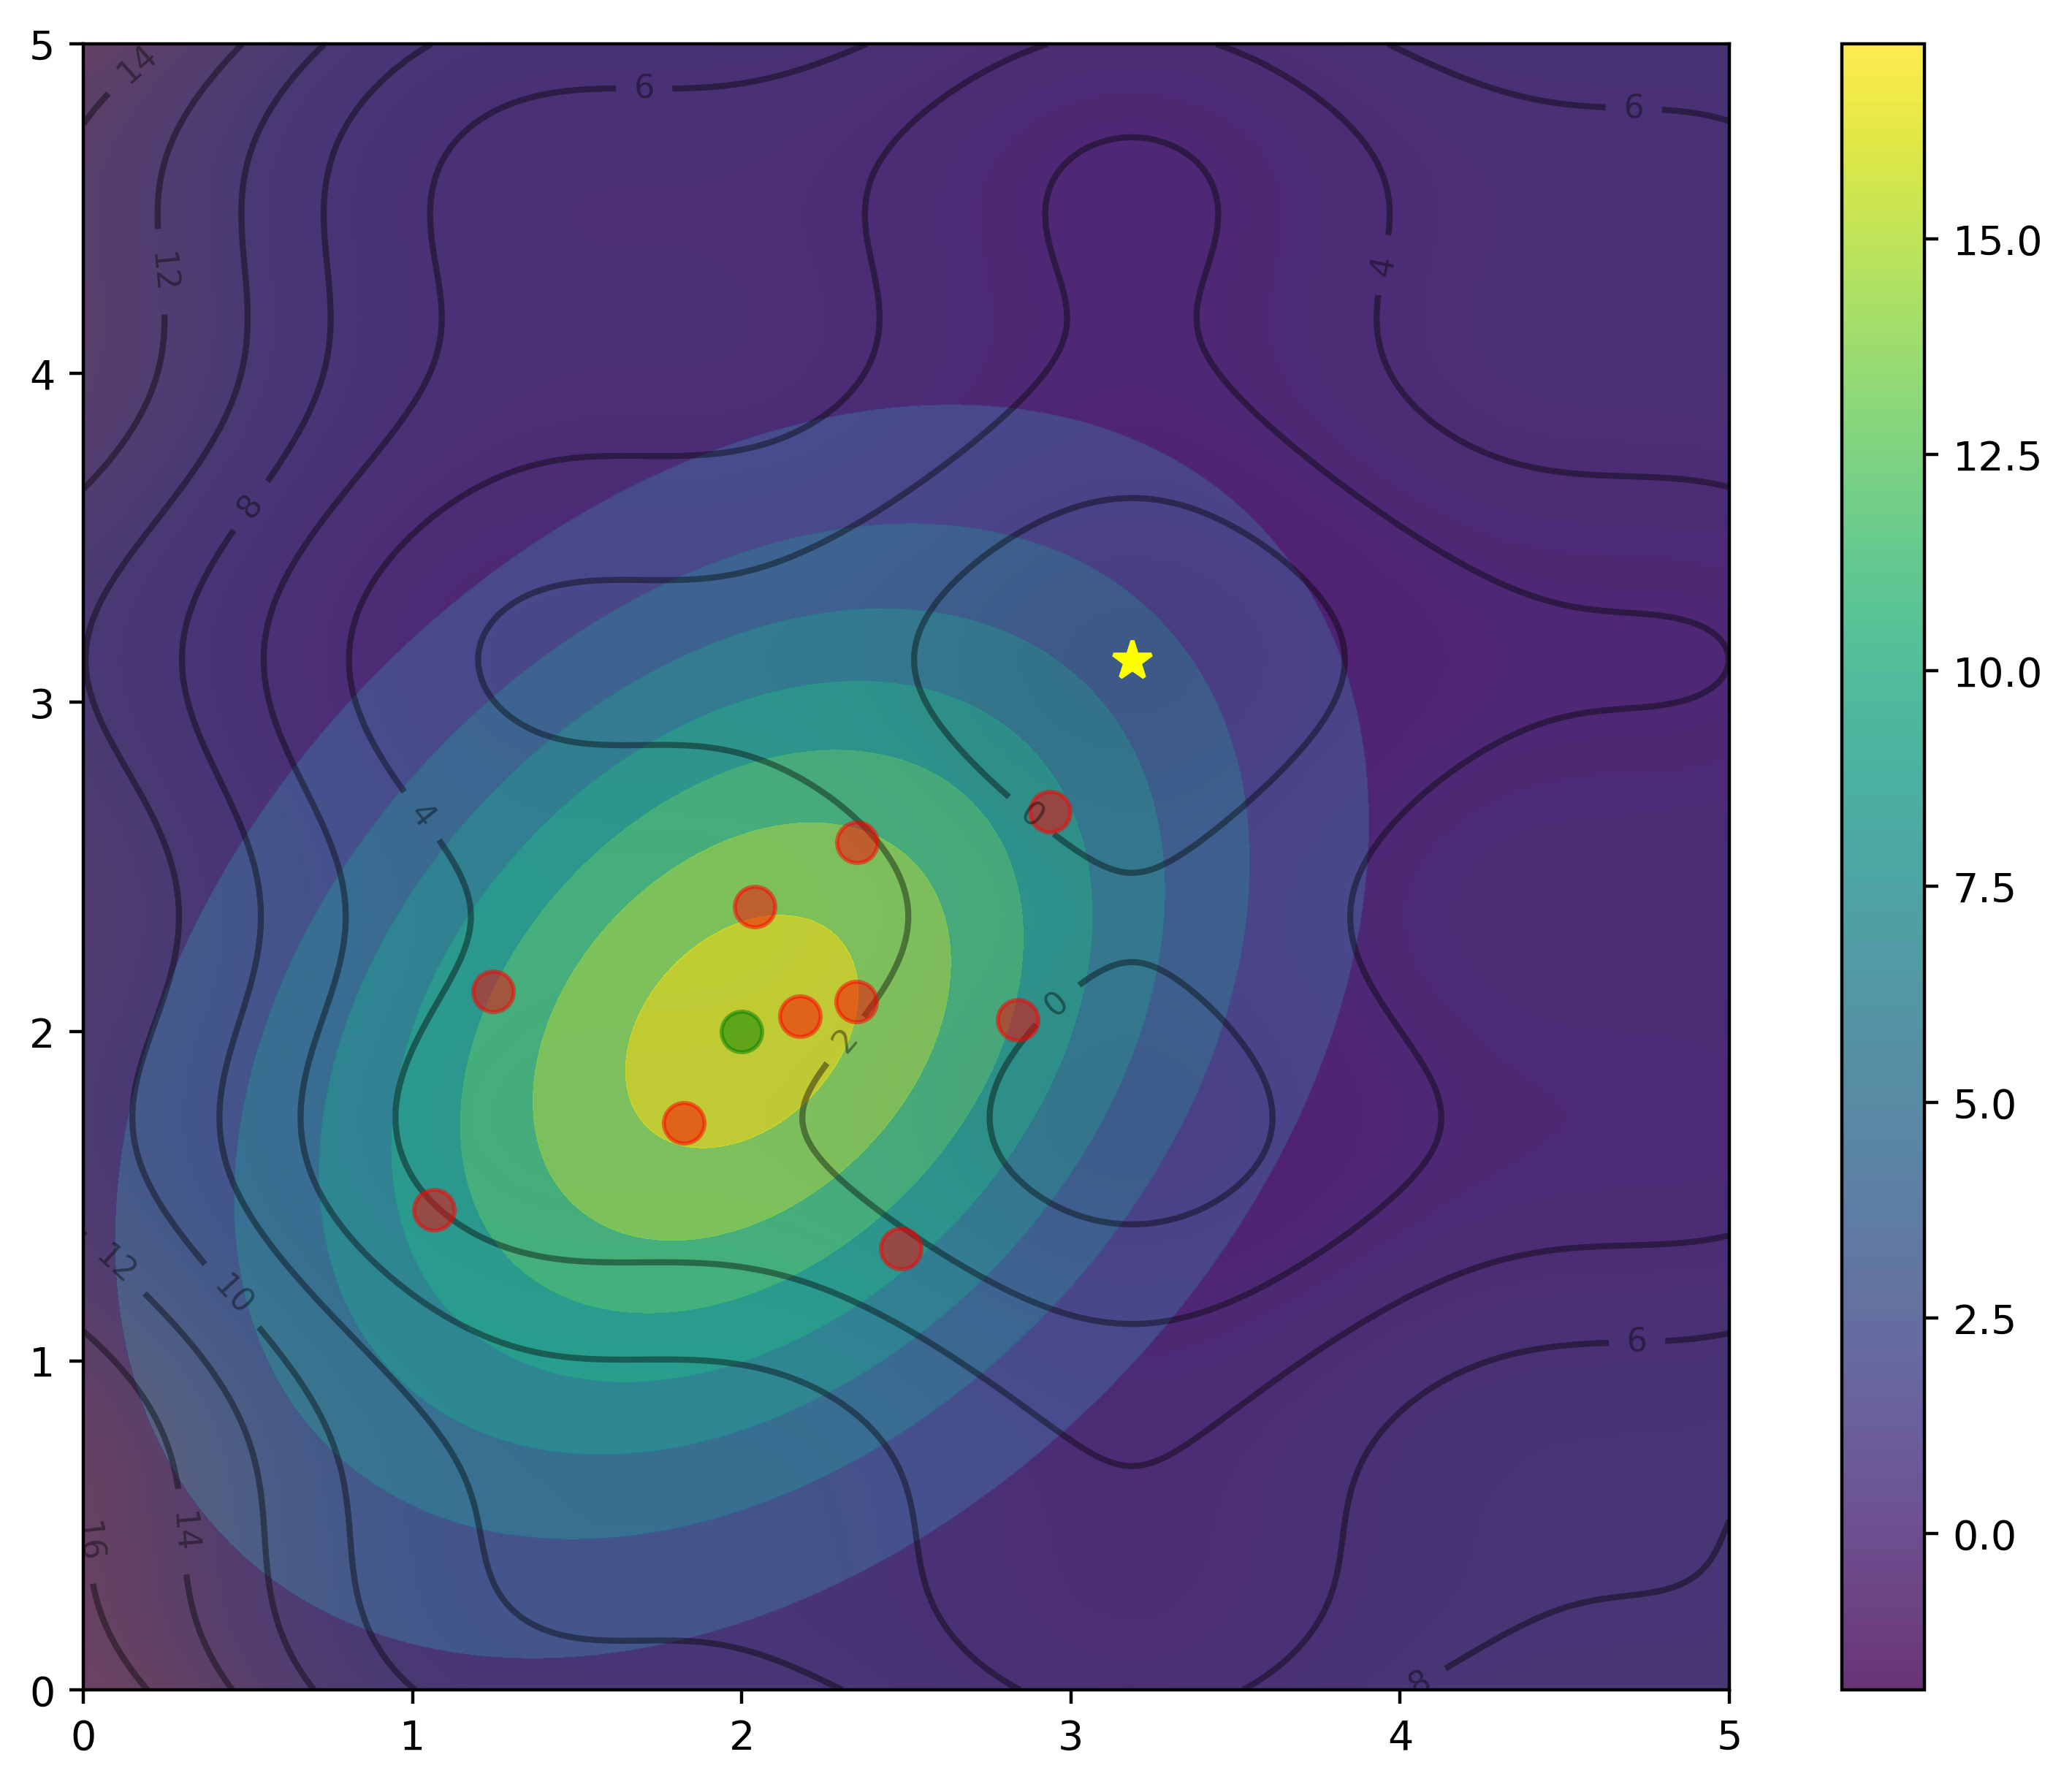
\includegraphics[scale=0.5]{image/theory/CMA.png}
   \caption{Visualización del proceso de optimización de $g(x, y)$ usando CMA-ES.}
  \label{fig:cma}
\end{figure}

\leonidas{
En la \autoref{fig:cma} se visualiza como CMA-ES optimiza $g(x, y)$ 
generando puntos dentro de la hyperelipse para explorar el espacio de búsqueda.
En siguientes iteraciones, de acuerdo a la exploración realizada la hyperelipse puede desplazarse y
contraerse o expandirse. Esto proceso es repetido iterativamente hasta que la hyperelipse termina 
reduciéndose a prácticamente un punto.
}


\subsection{\emph{Gradient Descent} (GD)}\label{sec:gradient-descent}

Este algoritmo comienza desde un punto inicial, en nuestro caso la matriz $\boldsymbol{P}$.
Luego, usa la derivada en ese punto para guiar su búsqueda iterativamente, 
esto lo realiza mediante la siguiente ecuación:

\begin{equation}
  \boldsymbol{P^{(t+1)}} \gets \boldsymbol{P^{(t)}} - \gamma \nabla \boldsymbol{P^{(t)}},
  \label{eq:gd-point}
\end{equation}

donde $t$ representa la iteración actual y $\gamma$ (conocido como el ratio de aprendizaje)
determina la magnitud de como actualizar $\boldsymbol{P^{(t)}}$. 
Particularmente, un enfoque razonable para buscar convergencia a 
un mínimo local es actualizar $\gamma$ en cada iteración mediante la ecuación

\begin{equation}
  \gamma^{(t+1)} = \frac{|(\boldsymbol{P^{(t)}}-\boldsymbol{P^{(t-1)}})^T(\nabla f(\boldsymbol{P^{(t)}})-\nabla f(\boldsymbol{P^{(t-1)}}))|}
  {||\nabla f(\boldsymbol{P^{(t)}})-\nabla f(\boldsymbol{P^{(t-1)}})||^2}.
  \label{eq:gd-gamma}
\end{equation}

Un detalle importante a señalar es que por simplicidad en la notación, 
la \autoref{eq:gd-gamma} se describió de esta manera;
sin embargo, en realidad debemos trabajar con la matriz $\boldsymbol{P}$ después de ser linealizada
para que las operaciones de esta ecuación estén bien definidas.
Mayores detalles del algoritmo se pueden encontrar en \cite{Demidova2020}.

\begin{figure}[ht]
  \centering
  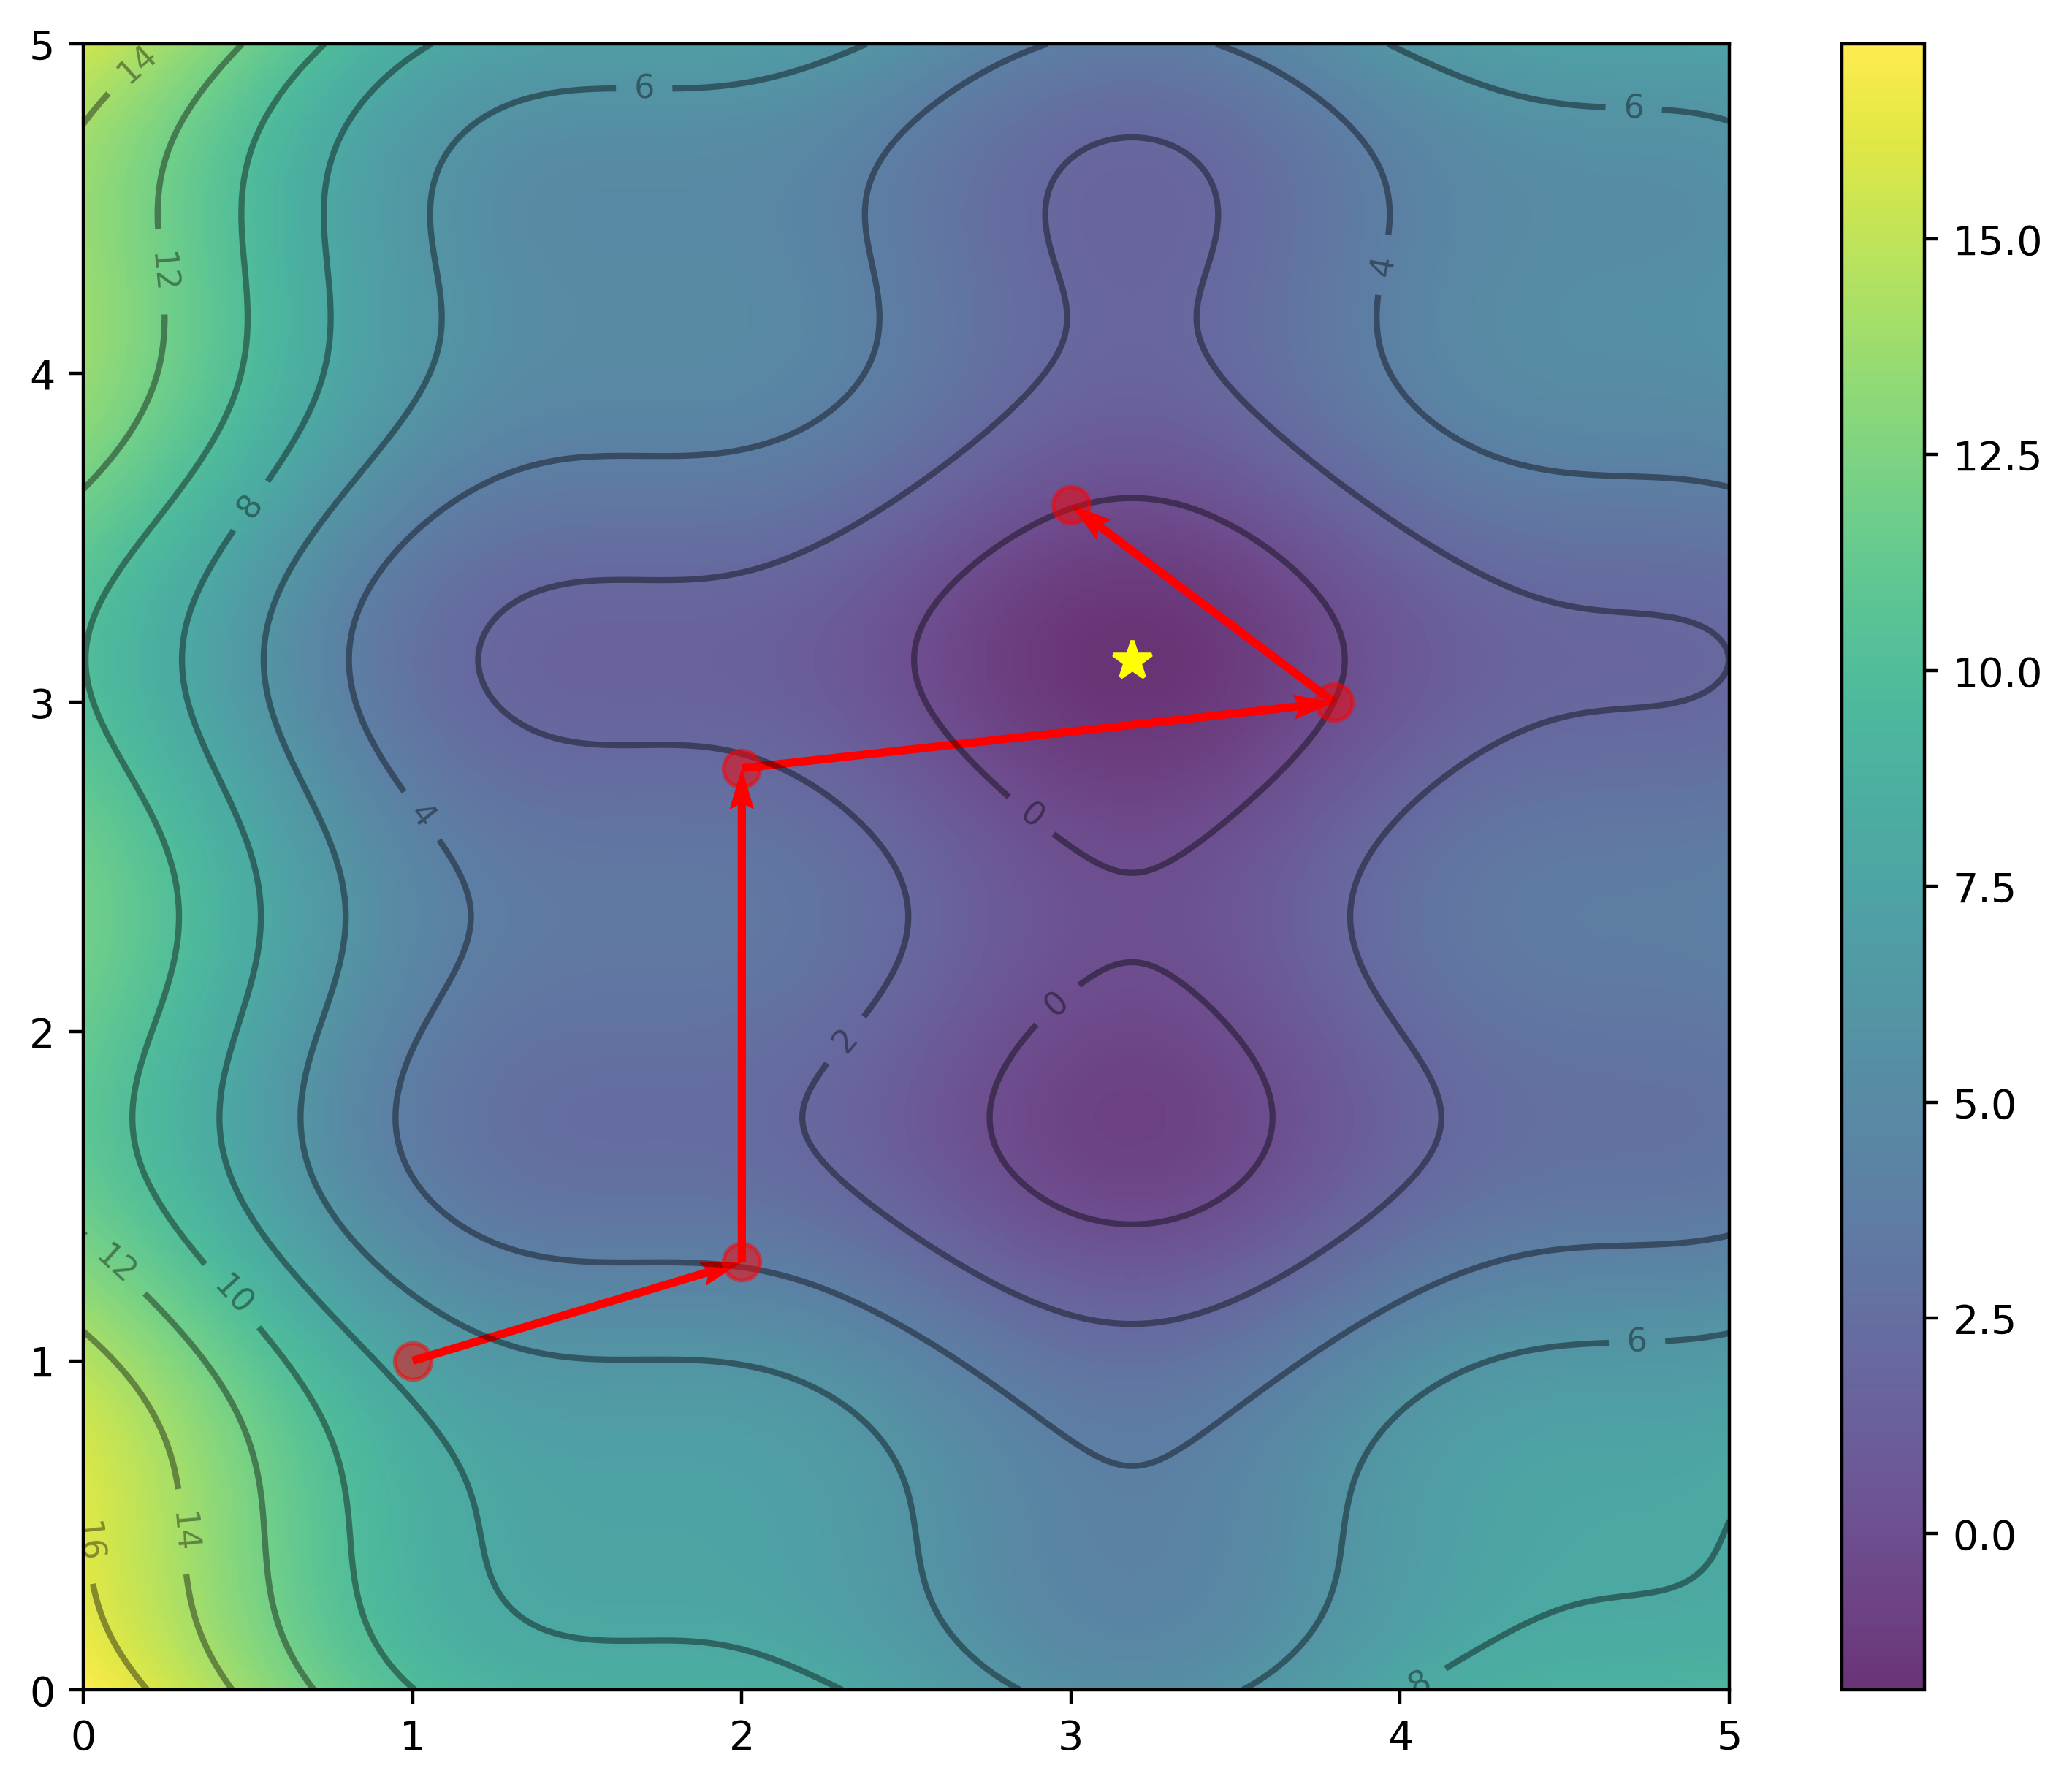
\includegraphics[scale=0.5]{image/theory/GD.png}
   \caption{Visualización del proceso de optimización de $g(x, y)$ usando GD.}
  \label{fig:gd}
\end{figure}

\leonidas{
En la \autoref{fig:gd} se visualiza como GD optimiza $g(x, y)$ 
El algoritmo comienza desde un punto y se mueve en dirección de la gradiente.
Como se observa, este algoritmo puede moverse eficientemente hacia
posiciones más óptimas; sin embargo, el algoritmo podría quedarse estancado en
óptimos locales.
}


\subsection{\emph{Method of Moving asymptotes} (MMA)}\label{sec:mma}

\emph{Method of moving asymptotes} (MMA) es un algoritmo de optimización
local basado en la gradiente, es decir, de primer orden. En esta sección usaremos
$\boldsymbol{\boldsymbol{x^{(i)}}}$ para representar la linealización de la $i-$ésima parametrización 
calculada ($\boldsymbol{P_i}$). Además, en este algoritmo se asume que tenemos $j = 1, 2, \dots, m^{+}$ inecuaciones 
($f_j(\boldsymbol{x}) < \overline{f_j}$) que deben cumplirse y la función a optimizar se denota como $f_0$.


Como se detalla en \cite{Svanberg1987}, el algoritmo se resume en estos 5 pasos:


\begin{enumerate}

  \item El escoge un punto inicial $\boldsymbol{x^{(0)}}$ y se inicializa $i \gets 0$.
    La elección de $\boldsymbol{x^{(0)}}$ puede ser un punto aleatorio.

  \item Se verifica que $\boldsymbol{x^{(0)}}$ no satisfaga criterios de convergencia, sino el programa
    termina.

  \item Se calcula $f_j(\boldsymbol{x^{(i)}})$ y $\nabla f_j(\boldsymbol{x^{(i)}})$ para $j = 0, 1, \dots, m^{+}$.

  \item Se utiliza multiplicadores de Lagrange a los resultados del paso anterior para plantear un
    nuevo subproblema.

  \item Se resuelve el subproblema obteniendo como solución $\boldsymbol{x^{(i)}}$.
        Se actualiza $i \gets i + 1$ y se regresa al paso 2.

\end{enumerate}

En la iteración $i$, para cada $f_j$ se escogen los parámetros
$L_t^{(i)}$ y $U_t^{(i)}$ tal que $L_t^{(i)} < x_t^{(i)} < U_t^{(i)}$ para $t = 1, 2, \dots,
n = dim(\boldsymbol{x^{(i)}})$. Luego, para $j = 0, 1, \dots, m^{+}$, se define:

\begin{equation}
  f_j^{(i)}(\boldsymbol{x}) = r_j^{(k)} + \displaystyle\sum_{t=1}^n\left(\frac{p_{jt}^{(i)}}{U_t^{(i)} - x_t}
  + \frac{q_{jt}^{(i)}}{x_t - L_t^{(i)}} \right),
\end{equation}

donde

\begin{equation}
  p_{jt}^{(i)} = \begin{cases*}
    (U_t^{(i)} - x_t^{(i)})^2 \partial f_j / \partial x_t, & si $0 < \partial f_j / \partial x_t$\\
    0, & en otro caso
  \end{cases*},
\end{equation}

\begin{equation}
  q_{jt}^{(i)} = \begin{cases*}
    -(x_t^{(u)} - L_t^{(i)})^2 \partial f_j / \partial x_t, & si $\partial f_j / \partial x_t < 0$\\
    0, & en otro caso
  \end{cases*},
\end{equation}


\begin{equation}
  r_j^{(i)} =  f_j(\boldsymbol{x^{(i)}}) + \displaystyle\sum_{t=1}^n\left(\frac{p_{jt}^{(i)}}{U_t^{(i)} - x_t^{(i)}}
  + \frac{q_{jt}^{(i)}}{x_t^{(i)} - L_t^{(i)}} \right),
\end{equation}

donde $\partial f_j / \partial x_t$ son evaluados en $\boldsymbol{x^{(i)}}$.
Es importante señalar que entre más cercanos a $x_t^{(i)}$ se encuentren $L_t^{(i)}$ y $U_t^{(i)}$,
entonces la segunda derivada toma un mayor valor, lo cual implica que la aproximación se vuelve más 
cercana al valor real. 
Los valores de estos parámetros van cambiando en cada iteración, esto es llamado mover asíntotas, de ahí el
nombre del algoritmo. Los detalles de como escoger estos parámetros son desarrollados en detalle
en \cite{Svanberg1987}.


En realidad en el presente trabajo usaremos una versión mejorada del MMA
conocida como \emph{Conservative Convex Separable Approximation} (CCSA) 
debido a su popularidad en optimización topológica, pero nos seguiremos refiriendo
al algoritmo como MMA por convención.
Esta variante tiene la particularidad de lograr converger a un mínimo local independientemente
del punto inicial. Los detalles se pueden revisar en \cite{Svanberg2002}.

\subsection{\emph{Limited-memory Broyden–Fletcher–Goldfarb–Shanno with boundaries} (L-BFGS-B)}\label{sec:lbfgsb}

\emph{Limited-memory Broyden–Fletcher–Goldfarb–Shanno with boundaries} (L-BFGS-B) es un algoritmo
de optimización de primer orden que suele utilizarse cuando no es práctico el cálculo de la matriz
Hesiana.

Sea $\boldsymbol{x_i}$ la parametrización $\boldsymbol{P}$ evaluada en la iteración $i$ 
luego de que esta matriz se linealice (i.e. se unieran sus vectores filas de manera consecutiva para 
formar un solo vector). Se define el siguiente modelo cuadrático:

\begin{equation}
m_i(\boldsymbol{x}) = f(\boldsymbol{x_i}) + (\nabla f(\boldsymbol{x_i}))^{T}(\boldsymbol{x_i}
- \boldsymbol{x}) + \frac{1}{2} (\boldsymbol{x_i}
- \boldsymbol{x})^{T} \boldsymbol{B_i} (\boldsymbol{x_i} - \boldsymbol{x}),
\end{equation}

\noindent donde $\boldsymbol{B_i}$ es una aproximación de la matriz Hesiana que usa una cantidad de memoria de orden
lineal.

El algoritmo L-BFGS-B aproximadamente minimiza $m_i(\boldsymbol{x})$ de forma iterativa.
La idea general del algoritmo se resume en los siguientes ocho pasos:

\begin{enumerate}

\item Dado un punto inicial $\boldsymbol{x_0}$, se inicializa $i \gets 0$ y 
  $\boldsymbol{B_0} \gets \boldsymbol{\mathbf{I}}$. Adicionalmente, se calcula
    $f(\boldsymbol{x_0})$ y $\nabla f(\boldsymbol{x_0})$. La elección de $x_0$ puede ser un punto aleatorio.

\item Si $||\boldsymbol{x_i} - \nabla f({\boldsymbol{x_i}})||_{\infty} < pgtol$, entonces el programa termina.
  El valor $pgtol$ es un parámetro del algoritmo, se recomienda que sea mayor a la raíz cuadrada de la
    precisión del computador donde se ejecute.

\item Se calcula el punto generalizado de Cauchy, este punto se define como el primer mínimo local 
  del camino definido por $\boldsymbol{x_i} - t \nabla f(\boldsymbol{x_i}), t \in \mathbb{R}$. 
    Los detalles de este cálculo se pueden encontrar en \cite{Byrd1995}.

\item Utilizando el resultado del anterior paso, se fijan ciertas dimensiones y se minimiza sobre las
  restantes. Producto de esta minimización se obtiene una solución aproximada $\overline{x}_{i+1}$.
    Así se define la direción de búsqueda $\boldsymbol{d_i} = \boldsymbol{\overline{x}_{i+1}} - \boldsymbol{x_i}$.
  Los detalles de los métodos de minimización sobre este subespacio se explican en \cite{Byrd1995}.

\item Se realiza una búsqueda en el camino definido por $\boldsymbol{x_i} - t \boldsymbol{d_i}, t \in \mathbb{R}$.
      La solución encontrada ($\lambda_i$) se utiliza para definir 
      $\boldsymbol{x_{i+1}} \gets \boldsymbol{x_{i}} + \lambda_i \boldsymbol{d_i}$.
      Es importante señalar que esta solución satisface

      \begin{equation}
      f(\boldsymbol{x_{i+1}}) \leq f(\boldsymbol{x_{i}}) + \alpha \lambda_i \nabla (f(\boldsymbol{x_{i}}))^T
        \boldsymbol{d_i},
      \end{equation}
      e intenta cumplir con la inecuación
      \begin{equation}
        |(\nabla f(\boldsymbol{x_{i+1}}))^T \boldsymbol{d_i}| < \beta |(\nabla f(\boldsymbol{x_{i}}))^T
        \boldsymbol{d_i}|,
      \end{equation}

      donde $\alpha$ y $\beta$ son parámetros del algoritmo. En el trabajo de \cite{Byrd1995} se
      utilizó $\alpha = 10^{-5}$ y $\beta = 0.9$ y se muestran los detalles de la búsqueda.


\item Se calcula $\nabla f(\boldsymbol{x_{i+1}})$.

\item Se calcula $\boldsymbol{B_{i+1}}$. Los detalles de este paso se pueden encontrar en \cite{Byrd1995}.

\item Se actualiza $i \gets i + 1$ y se regresa al paso 2.

\end{enumerate}


Adicionalmente, para el cálculo de la aproximación $\boldsymbol{B}$ el algoritmo recibe un parámetro
$\overline{m}$ para guardar información relacionada con la gradiente de solo las últimas $\overline{m}$ 
iteraciones. Para este párametro valores pequeños ($3 \leq \overline{m} \leq 20$) son recomendados.
Así, el algoritmo es adecuado para problemas con dimensiones elevadas debido a que
ha mostrado buen desempeño en distintos problemas utilizando bajos recursos de memoria
($O(\overline{m}n)$) y de tiempo de ejecución por iteración ($O(\overline{m}^2n)$) 
\citep{Zhu1997}.

Para una descripción más detallada del algoritmo, revisar los trabajos de \cite{Byrd1995} y \cite{Zhu1997}.

\subsection{G-CMA-ES}\label{sec:g-cma-es}

Esta es una variación de la \autoref{sec:cma-es}. El algoritmo es el mismo que el CMA-ES,
pero antes de ejecutar la línea 3 del Algoritmo \ref{alg:CMA}, se calcula la
gradiente de la actual media (i.e., $\nabla f(\mu)$). Con este valor se busca guíar
mejor las operaciones de la hyperelipse.
Los detalles a profundidad se pueden encontrar en \cite{Nikolaus2021}.

\subsection{G-PSO}\label{sec:g-pso}

Esta es una variación propuesta en la presente tesis.
Basándonos en el trabajo de \cite{Demidova2020}, después de cada iteración
del Algoritmo \ref{alg:PSO} (i.e., línea 4), añadimos los siguientes pasos:

\begin{enumerate}
  \item Se ejecuta el algoritmo GD (\autoref{sec:gradient-descent}) tomando como punto inicial
       $\boldsymbol{P_{b}}$. Este algoritmo se ejecuta por $k\_gd$ iteraciones con un 
       parámetro inicial de $\gamma$. El algoritmo se guarda como $\boldsymbol{P_{b}^{+}}$. 
  \item Se actualiza la mejor posición encontrada globalmente entre $\boldsymbol{P_{b}^{+}}$ y 
       $\boldsymbol{P_{b}}$.
\end{enumerate}

La idea detrás de esta variante es asegurar que la mejor solución global alcance un mejor resultado
y que guíe a las demás partículas.
Así, manteniendo el enfoque de un algoritmo de optimización global, se espera que este algoritmo
no se estanque fácilmente en óptimos locales.


\subsection{G-GA}\label{sec:g-ga}

Similar al G-PSO, después de cada iteración del Algoritmo \ref{alg:GA} (i.e. 5), se escoge dos
elementos aleatorios para actualizarlos aplicándoles GD por $k\_gd$ iteraciones con un parámetro inicial
de $\gamma$.
Se escoge dos elementos y no solo uno para asegurar que los resultados de aplicar GD
se compartan con los demás individuos en pocas iteraciones, similar a lo que sucede en \autoref{sec:g-pso}.


En el presente capítulo se ha descrito la teoría necesaria para optimizar el diseño de un
un \emph{bend} y WDM.
Esto ha implicado la explicación de la parametrización basada en píxeles,
el uso de SPINS-B y transformaciones utilizadas en la optimización topológica robusta.
Además, se ha desarrollado la explicación de tres algoritmos que no necesitan calcular la gradiente:
(i) GA, (ii) PSO y (iii) CMA-ES. Asimismo, se describió seis algoritmos de primer orden 
(que usan la gradiente): (i) GD, (ii) MMA y (iii) L-BFGS-B, (iv) G-CMA-ES, (v) G-PSO y (vi) G-GA.
Siendo los últimos dos algoritmos contribuciones del presente trabajo de investigación.
Los conceptos presentados en este capítulo serán de utilidad para entender la metodología descrita en el
\autoref{chapter:methodology}.
